% Options for packages loaded elsewhere
% Options for packages loaded elsewhere
\PassOptionsToPackage{unicode}{hyperref}
\PassOptionsToPackage{hyphens}{url}
\PassOptionsToPackage{dvipsnames,svgnames,x11names}{xcolor}
%
\documentclass[
  12pt,
  a4paper,
]{article}
\usepackage{xcolor}
\usepackage[margin=2.25cm]{geometry}
\usepackage{amsmath,amssymb}
\setcounter{secnumdepth}{5}
\usepackage{iftex}
\ifPDFTeX
  \usepackage[T1]{fontenc}
  \usepackage[utf8]{inputenc}
  \usepackage{textcomp} % provide euro and other symbols
\else % if luatex or xetex
  \usepackage{unicode-math} % this also loads fontspec
  \defaultfontfeatures{Scale=MatchLowercase}
  \defaultfontfeatures[\rmfamily]{Ligatures=TeX,Scale=1}
\fi
\usepackage{lmodern}
\ifPDFTeX\else
  % xetex/luatex font selection
  \setmainfont[]{Times New Roman}
\fi
% Use upquote if available, for straight quotes in verbatim environments
\IfFileExists{upquote.sty}{\usepackage{upquote}}{}
\IfFileExists{microtype.sty}{% use microtype if available
  \usepackage[]{microtype}
  \UseMicrotypeSet[protrusion]{basicmath} % disable protrusion for tt fonts
}{}
\usepackage{setspace}
\makeatletter
\@ifundefined{KOMAClassName}{% if non-KOMA class
  \IfFileExists{parskip.sty}{%
    \usepackage{parskip}
  }{% else
    \setlength{\parindent}{0pt}
    \setlength{\parskip}{6pt plus 2pt minus 1pt}}
}{% if KOMA class
  \KOMAoptions{parskip=half}}
\makeatother
% Make \paragraph and \subparagraph free-standing
\makeatletter
\ifx\paragraph\undefined\else
  \let\oldparagraph\paragraph
  \renewcommand{\paragraph}{
    \@ifstar
      \xxxParagraphStar
      \xxxParagraphNoStar
  }
  \newcommand{\xxxParagraphStar}[1]{\oldparagraph*{#1}\mbox{}}
  \newcommand{\xxxParagraphNoStar}[1]{\oldparagraph{#1}\mbox{}}
\fi
\ifx\subparagraph\undefined\else
  \let\oldsubparagraph\subparagraph
  \renewcommand{\subparagraph}{
    \@ifstar
      \xxxSubParagraphStar
      \xxxSubParagraphNoStar
  }
  \newcommand{\xxxSubParagraphStar}[1]{\oldsubparagraph*{#1}\mbox{}}
  \newcommand{\xxxSubParagraphNoStar}[1]{\oldsubparagraph{#1}\mbox{}}
\fi
\makeatother


\usepackage{longtable,booktabs,array}
\newcounter{none} % for unnumbered tables
\usepackage{calc} % for calculating minipage widths
% Correct order of tables after \paragraph or \subparagraph
\usepackage{etoolbox}
\makeatletter
\patchcmd\longtable{\par}{\if@noskipsec\mbox{}\fi\par}{}{}
\makeatother
% Allow footnotes in longtable head/foot
\IfFileExists{footnotehyper.sty}{\usepackage{footnotehyper}}{\usepackage{footnote}}
\makesavenoteenv{longtable}
\usepackage{graphicx}
\makeatletter
\newsavebox\pandoc@box
\newcommand*\pandocbounded[1]{% scales image to fit in text height/width
  \sbox\pandoc@box{#1}%
  \Gscale@div\@tempa{\textheight}{\dimexpr\ht\pandoc@box+\dp\pandoc@box\relax}%
  \Gscale@div\@tempb{\linewidth}{\wd\pandoc@box}%
  \ifdim\@tempb\p@<\@tempa\p@\let\@tempa\@tempb\fi% select the smaller of both
  \ifdim\@tempa\p@<\p@\scalebox{\@tempa}{\usebox\pandoc@box}%
  \else\usebox{\pandoc@box}%
  \fi%
}
% Set default figure placement to htbp
\def\fps@figure{htbp}
\makeatother


% definitions for citeproc citations
\NewDocumentCommand\citeproctext{}{}
\NewDocumentCommand\citeproc{mm}{%
  \begingroup\def\citeproctext{#2}\cite{#1}\endgroup}
\makeatletter
 % allow citations to break across lines
 \let\@cite@ofmt\@firstofone
 % avoid brackets around text for \cite:
 \def\@biblabel#1{}
 \def\@cite#1#2{{#1\if@tempswa , #2\fi}}
\makeatother
\newlength{\cslhangindent}
\setlength{\cslhangindent}{1.5em}
\newlength{\csllabelwidth}
\setlength{\csllabelwidth}{3em}
\newenvironment{CSLReferences}[2] % #1 hanging-indent, #2 entry-spacing
 {\begin{list}{}{%
  \setlength{\itemindent}{0pt}
  \setlength{\leftmargin}{0pt}
  \setlength{\parsep}{0pt}
  % turn on hanging indent if param 1 is 1
  \ifodd #1
   \setlength{\leftmargin}{\cslhangindent}
   \setlength{\itemindent}{-1\cslhangindent}
  \fi
  % set entry spacing
  \setlength{\itemsep}{#2\baselineskip}}}
 {\end{list}}
\usepackage{calc}
\newcommand{\CSLBlock}[1]{\hfill\break\parbox[t]{\linewidth}{\strut\ignorespaces#1\strut}}
\newcommand{\CSLLeftMargin}[1]{\parbox[t]{\csllabelwidth}{\strut#1\strut}}
\newcommand{\CSLRightInline}[1]{\parbox[t]{\linewidth - \csllabelwidth}{\strut#1\strut}}
\newcommand{\CSLIndent}[1]{\hspace{\cslhangindent}#1}



\setlength{\emergencystretch}{3em} % prevent overfull lines

\providecommand{\tightlist}{%
  \setlength{\itemsep}{0pt}\setlength{\parskip}{0pt}}



 


\usepackage{booktabs}
\usepackage{caption}
\usepackage{longtable}
\usepackage{colortbl}
\usepackage{array}
\usepackage{anyfontsize}
\usepackage{multirow}
\usepackage{needspace}
% In the appendix a heading, its caption and the first rows of a table
% stay on one page (the flag is set at the start of the appendix).
\newif\ifappendixpages
\AddToHook{cmd/section/before}{\ifappendixpages\Needspace*{10\baselineskip}\fi}
\AddToHook{cmd/subsection/before}{\ifappendixpages\Needspace*{10\baselineskip}\fi}
\AddToHook{cmd/subsubsection/before}{\ifappendixpages\Needspace*{10\baselineskip}\fi}
\makeatletter
% Space, not content: a float shares its page with text unless it
% fills 85% of it; displays, headings and captions take smaller
% skips; the paragraph gap is half of parskip's default.
\renewcommand{\topfraction}{.9}
\renewcommand{\bottomfraction}{.7}
\renewcommand{\textfraction}{.1}
\renewcommand{\floatpagefraction}{.85}
\g@addto@macro\normalsize{%
  \setlength\abovedisplayskip{6pt plus 2pt minus 4pt}%
  \setlength\belowdisplayskip{6pt plus 2pt minus 4pt}%
  \setlength\abovedisplayshortskip{0pt plus 2pt}%
  \setlength\belowdisplayshortskip{3pt plus 2pt minus 2pt}}
\renewcommand\section{\@startsection{section}{1}{\z@}%
  {-2.25ex \@plus -1ex \@minus -.2ex}{1.2ex \@plus .2ex}%
  {\normalfont\Large\bfseries}}
\renewcommand\subsection{\@startsection{subsection}{2}{\z@}%
  {-2ex \@plus -.75ex \@minus -.2ex}{.9ex \@plus .2ex}%
  {\normalfont\large\bfseries}}
\renewcommand\subsubsection{\@startsection{subsubsection}{3}{\z@}%
  {-1.75ex \@plus -.5ex \@minus -.2ex}{.7ex \@plus .2ex}%
  {\normalfont\normalsize\bfseries}}
\AtBeginDocument{\setlength{\parskip}{3.5pt plus 1pt}}
% Appendix tables and figures are set in place rather than floated,
% so a table breaks across pages under its caption; a figure and its
% caption share one box.
\AtBeginDocument{%
  \renewenvironment{atbl}{\par\if@nobreak\else\Needspace*{6\baselineskip}\fi\def\@captype{atbl}\def\fps@table{H}}{\par}%
  \renewenvironment{afig}{\par\if@nobreak\else\Needspace*{6\baselineskip}\fi\def\@captype{afig}\noindent\begin{minipage}{\linewidth}}{\end{minipage}\par}%
  % panels (a), (b) of an appendix float are numbered within it
  \@ifpackageloaded{subcaption}%
    {\DeclareCaptionSubType{atbl}\DeclareCaptionSubType{afig}}{}%
  \captionsetup{skip=6pt}%
  \captionsetup[table]{font=normalsize}%
  \floatplacement{figure}{!htbp}}
% Tables other than gt's, which set their own size, in 8pt.
\AddToHook{env/longtable/begin}{\fontsize{8pt}{9.6pt}\selectfont}
\setlength{\tabcolsep}{3.5pt}
% The article class sets the abstract as a quotation, which indents
% its first line and every paragraph. Same margins, no indents.
\renewenvironment{abstract}{%
  \small
  \begin{center}{\bfseries\abstractname\vspace{-.5em}\vspace{\z@}}\end{center}%
  \list{}{\listparindent\z@ \itemindent\z@ \rightmargin\leftmargin
          \parsep 6pt \@plus 2pt}%
  \item\relax}{\endlist}
% Reference entries flush left, no hanging indent.
\AtBeginDocument{\ifdefined\cslhangindent\setlength{\cslhangindent}{0pt}\fi}
\makeatother
\makeatletter
\@ifpackageloaded{float}{}{\usepackage{float}}
\floatstyle{plain}
\@ifundefined{c@chapter}{\newfloat{atbl}{h}{loatbl}}{\newfloat{atbl}{h}{loatbl}[chapter]}
\floatname{atbl}{Appendix Table}
\floatstyle{plaintop}
\restylefloat{atbl}
\newcommand*\listofatbls{\listof{atbl}{List of Appendix Tables}}
\makeatother
\makeatletter
\@ifpackageloaded{float}{}{\usepackage{float}}
\floatstyle{plain}
\@ifundefined{c@chapter}{\newfloat{afig}{h}{loafig}}{\newfloat{afig}{h}{loafig}[chapter]}
\floatname{afig}{Appendix Figure}
\newcommand*\listofafigs{\listof{afig}{List of Appendix Figures}}
\makeatother
\makeatletter
\@ifpackageloaded{caption}{}{\usepackage{caption}}
\AtBeginDocument{%
\ifdefined\contentsname
  \renewcommand*\contentsname{Table of contents}
\else
  \newcommand\contentsname{Table of contents}
\fi
\ifdefined\listfigurename
  \renewcommand*\listfigurename{List of Figures}
\else
  \newcommand\listfigurename{List of Figures}
\fi
\ifdefined\listtablename
  \renewcommand*\listtablename{List of Tables}
\else
  \newcommand\listtablename{List of Tables}
\fi
\ifdefined\figurename
  \renewcommand*\figurename{Figure}
\else
  \newcommand\figurename{Figure}
\fi
\ifdefined\tablename
  \renewcommand*\tablename{Table}
\else
  \newcommand\tablename{Table}
\fi
}
\@ifpackageloaded{float}{}{\usepackage{float}}
\floatstyle{ruled}
\@ifundefined{c@chapter}{\newfloat{codelisting}{h}{lop}}{\newfloat{codelisting}{h}{lop}[chapter]}
\floatname{codelisting}{Listing}
\newcommand*\listoflistings{\listof{codelisting}{List of Listings}}
\makeatother
\makeatletter
\makeatother
\makeatletter
\@ifpackageloaded{caption}{}{\usepackage{caption}}
\@ifpackageloaded{subcaption}{}{\usepackage{subcaption}}
\makeatother
\usepackage{bookmark}
\IfFileExists{xurl.sty}{\usepackage{xurl}}{} % add URL line breaks if available
\urlstyle{same}
\hypersetup{
  pdftitle={Balancing weights against maximum likelihood propensity scores: a simulation study of balnet across sample size{,} overlap{,} dimension and penalty choice},
  pdfauthor={Otis Sandford},
  colorlinks=true,
  linkcolor={blue},
  filecolor={Maroon},
  citecolor={Blue},
  urlcolor={Blue},
  pdfcreator={LaTeX via pandoc}}


\title{Balancing weights against maximum likelihood propensity scores: a
simulation study of \texttt{balnet} across sample size, overlap,
dimension and penalty choice}
\usepackage{etoolbox}
\makeatletter
\providecommand{\subtitle}[1]{% add subtitle to \maketitle
  \apptocmd{\@title}{\par {\large #1 \par}}{}{}
}
\makeatother
\subtitle{ETC5860 Masters thesis, Monash University. Supervisor: Erik
Sverdrup}
\author{Otis Sandford}
\date{2026-10-16}
\begin{document}
\maketitle
\begin{abstract}
Maximum likelihood fits propensity scores to predict treatment,
balancing weights to balance covariates directly. \texttt{balnet} fits
balancing weights by a lasso-penalised balancing loss whose path runs to
exact balance or stops short where infeasible. We compare
\texttt{balnet} with cross-validated lasso MLE weights, alone and
augmented, by simulation across sample size, overlap, dimension past
\(p = n\), confounder density and outcome signal, with and without
misspecification. Balancing weights have lower RMSE throughout, by a
third to two thirds on average, except noisy outcomes and the poorest
overlap. Whether the path reaches exact balance decides what else helps.
Augmentation adds nothing there and restores the lead where it stops
short. A second study finds stopping inside the path lowers RMSE for
noisy outcomes or, once augmented, limited overlap. Cross-validating the
balancing loss captures this most often, though none is best in more
than three cells in ten. We recommend augmented balancing weights tuned
this way.

\emph{Keywords:} balancing weights; propensity score; inverse
probability weighting; lasso; Monte Carlo simulation.
\end{abstract}


\setstretch{1.15}
\section{Introduction}\label{introduction}

Much of the evidence on programmes, treatments and interventions is
observational. Without randomisation, the groups compared differ in
their pre-treatment characteristics, and those differences, not the
treatment, may explain any gap in outcomes.

The standard approach is to assume conditional independence, meaning
that once the relevant pre-treatment characteristics are controlled for,
treatment allocation is as good as random. Key to this is the propensity
score, the probability of receiving treatment given the observed
covariates (Rosenbaum and Rubin 1983). One use of the score is
inverse-propensity weighting (IPW), which weights each unit by the
inverse of its estimated probability of the treatment it received. In
medical research its use has increased rapidly, for example in comparing
treatments from hospital records where patients were never randomised
(Austin and Stuart 2015; Ben-Michael and Keele 2023). In economics, IPW
is used to evaluate programmes such as job training, where the effect on
participants' earnings must be recovered from a non-experimental
comparison group (Busso et al. 2014).

In practice the score is unknown and must be estimated. The usual
estimator is logistic regression fit by maximum likelihood (MLE). It
chooses the parameters of the propensity model so that the fitted score
predicts the observed treatment assignment as well as possible (Wager
2024). The goal of weighting here however, is not to predict treatment
assignment accurately but to balance covariates for comparable treatment
groups (Zhao 2019).

While IPW with the oracle propensity score balances covariate means
exactly, MLE-estimated propensity scores do not generally achieve this,
even without model misspecification (Wager 2024; Sverdrup and Hastie
2026). Under misspecification or in small samples, small estimation
errors are amplified by inversion of the propensity score and can
produce severe imbalance and biased estimates (Ben-Michael et al. 2021).
This problem is compounded by weight instability, as observations with
small propensity scores receive disproportionately large weights,
inflating variance and leading researchers to ad hoc solutions
(Chattopadhyay et al. 2020). Furthermore, these fixes presume a balance
check that in a review of applied medical studies using IPW, most did
not make (Austin and Stuart 2015).

Instead of modelling the score, covariate balancing methods choose the
weights to target directly the balance that IPW requires. The covariate
balancing propensity score (CBPS) applies this within a propensity
model, selecting its parameters to satisfy the sample balance conditions
(Imai and Ratkovic 2014). As a result, their estimates tend to be more
robust to model misspecification and more efficient than those from MLE
weights (Chattopadhyay et al. 2020). Under a correctly specified linear
outcome and logistic propensity model, this efficiency is exact and IPW
with balancing weights is \(\sqrt{n}\)-consistent with lower variance
than even the oracle IPW (Wager 2024).

The theoretical case for covariate balancing is well established, but
most implementations struggle with large or high-dimensional data. CBPS
and entropy balancing approaches both enforce exact balance conditions,
which become unworkable in large-scale data settings (Fong et al. 2022;
Sverdrup and Hastie 2026). Stable balancing weights from Zubizarreta
(2015) require a maximum imbalance tolerance to be set before estimation
and must be re-solved if this tolerance is unattainable or the
bias-variance tradeoff is unattractive (Sverdrup and Hastie 2026). Zhao
(2019) shows balancing estimators can generally be expressed as
minimising a covariate balancing loss function, which opens them to
lasso and other penalties. RCAL from Tan (2020b) implements lasso
regularisation for a covariate balancing loss function, but as the
package is written in R it struggles computationally with large data.

Like balancing approaches, doubly robust estimators offer protection
against misspecification. These estimators, referred to as augmented
estimators, combine the weights with an outcome model and remain
consistent if either the propensity model or the outcome model is
correctly specified (Ding 2024). The standard version is the augmented
IPW (AIPW) estimator. It corrects the regression estimate by applying
the IPW weights to the outcome model's residuals and adding their
average (Robins et al. 1994). Where exact balance is out of reach, AIPW
has outperformed unaugmented balancing weights (Athey et al. 2018).

Much recent work builds doubly robust estimators for the balancing
approach, many obtaining the weights by optimising for balance directly
rather than by first estimating a propensity score (Wang and Zubizarreta
2020; Hirshberg and Wager 2021; Bruns-Smith et al. 2026). These
augmented estimators therefore sit outside the class of covariate
balancing propensity scores that Zhao (2019) unifies. Within that class,
Tan's augmented estimator fits the outcome model with weights from the
same propensity score, so changing the weights changes the outcome model
too (Tan 2020a).\footnote{Tan's estimator refits the outcome model
  whenever the weights change, so a comparison between weights would
  also be a comparison between outcome models. Applying it here would
  confound Study 1, which compares across weighting estimators.}
Bruns-Smith et al. (2026) discuss a general augmented balancing weight
(ABW) estimator, where the outcome model is held fixed and the IPW
weights are replaced by balancing weights. Here, when both models are
linear in the same covariates, ABW is a single regression combining the
outcome model and OLS, which collapses to OLS at exact balance (Wager
2024). For weights from the covariate balancing loss above, which come
through a logistic link, this collapse holds only up to an approximation
error.

Of the balancing implementations above, \texttt{balnet} from Sverdrup
and Hastie (2026) applies modern optimisation techniques to the
regularised covariate balancing loss. Like RCAL it uses lasso
regularisation, but through a core solver written in C++ that scales to
large and high-dimensional data. The solver also supports ridge and
elastic net penalties, which Study 2 uses. Its path for
\(n = 100{,}000\) and \(p = 500\) computes in under a minute, while
alternative balancing packages failed to produce results within an hour.
Under lasso regularisation the penalty parameter \(\lambda\) is
equivalent to the maximum allowable covariate imbalance, so its
regularisation path provides a practical diagnostic for overlap and lets
the analyst set the imbalance to tolerate (Sverdrup and Hastie 2026).
The path ends at the target imbalance rather than at exact balance, and
truncates earlier where that target is infeasible. The imbalance left
over can then be handed to an outcome model (Wager 2024).

For modelling approaches it is standard practice to choose \(\lambda\)
by cross-validation (CV) of the prediction error, a choice one would
reasonably expect to extend to balancing loss approaches.\footnote{Both
  RCAL and \texttt{balnet} provide a CV setting with tunable folds in
  their base package.} However, for balancing weights recent work
cautions against applying cross-validation naively, finding that no
tuning rule is uniformly best (Bruns-Smith et al. 2026).

For balancing methods the held-out loss becomes the balancing loss or
the remaining covariate imbalance. CV then assumes the held-out loss is
an unbiased estimate of the error in the estimated effect, but the
penalty trades observable variance against unobservable bias, a trade CV
cannot reliably make (Tan 2020b; Bruns-Smith et al. 2026; Athey et al.
2018). Following the reasoning behind balancing weights, Wang and
Zubizarreta (2020) score balance on bootstrap samples over a grid of
approximate balance tolerances and find that under poor overlap exact
balance is not always optimal. On the \texttt{balnet} path this becomes
a question of where to set \(\lambda\), or whether to set it at all, as
by construction its truncated path already produces approximate
balancing weights when exact balance is not feasible.

Study 1 asks to what degree and when balancing weights improve on MLE
weights, whether used alone or in an augmented estimator. Study 2 then
asks where \texttt{balnet}'s path endpoint does not minimise root mean
squared error (RMSE), and whether at those points any selector beats it.
Across both studies the dividing line is whether the \texttt{balnet}
path reaches exact balance, which with the outcome signal tells the
analyst when balancing weights, augmentation and a selector each pay.

\section{Aims}\label{aims}

\subsection{Study 1}\label{study-1}

Our first study aims to guide the choice between balancing weights and
MLE weights, whether used alone or in an augmented estimator. The
settings that follow vary the sample size, overlap, dimension, the
number and correlation of confounders, and the strength of the outcome
signal. Each is run under both a correctly specified and a misspecified
propensity score. Following Tan (2020b), we focus on how the two sets of
weights perform relative to each other across these settings and over
three outcome functions.

Both sets of weights are also augmented with the same lasso outcome
model, so ABW and AIPW differ only in their weights. Comparing the two
shows whether differences between balancing and MLE weights hold once an
outcome model is added. At exact balance, \texttt{balnet}\(_{10^{-4}}\)
differs from OLS by the approximation error of its logistic weights
(Bruns-Smith et al. 2026). We track this error where OLS can be fitted
and the path reaches its target.

\textbf{Sample size:} Under a correctly specified propensity score both
approaches are consistent (Wager 2024). For a linear outcome, IPW with
balancing weights is expected to have lower variance than even IPW with
the true propensity score. Here we ask how the sample size affects the
relative performance of \texttt{balnet}\(_{10^{-4}}\) and
\texttt{cv.glmnet}, a baseline for the later comparisons.

Under a misspecified propensity score, IPW estimators can converge away
from the true estimand, and with MLE weights their bias and RMSE have
been found to worsen as \(n\) grows (Waernbaum and Pazzagli 2023; Kang
and Schafer 2007). We therefore ask whether the bias of
\texttt{cv.glmnet} settles as \(n\) rises to \(10^6\), and how
\texttt{balnet}\(_{10^{-4}}\) compares. We also track AIPW, which has
been found to compound errors when both models are wrong (Kang and
Schafer 2007). Where a bias settles while the sampling error shrinks,
coverage must collapse with \(n\), which we report at the empirical SE
(Morris et al. 2019).

\textbf{Overlap:} We then compare the two sets of weights as overlap
degrades, meaning that treated and control units increasingly lack
counterparts with similar propensity scores. We also include levels at
which overlap is practically violated, as defined in the data-generating
mechanism.

With a correctly specified outcome model, AIPW has outperformed
unaugmented approximate balancing weights at both overlap levels studied
(Athey et al. 2018). Under poor overlap and a misspecified outcome
model, however, unaugmented approximate balancing weights have produced
lower RMSE than AIPW (Chattopadhyay et al. 2020). Besides these swapped
signs, we ask how \texttt{balnet}\(_{10^{-4}}\) performs once exact
balance is out of reach, as exact balancing weights can become
infeasible under poor overlap (Hainmueller 2012; Sverdrup and Hastie
2026).

\textbf{High-dimensional settings:} In healthcare especially, propensity
scores are fitted to a large number of covariates, as in database
studies ({Wyss et al.} 2026). By raising the number of covariates to
\(p/n = 4\) we cover these settings, which force the MLE weights to
select four confounders within thousands of covariates and the balancing
weights to balance thousands. Here we also ask how the balancing loss
behaves as \(p\) grows.

Firstly, exact balance is expected to fail for
\texttt{balnet}\(_{10^{-4}}\) around \(p/n = 0.5\), so that its path
stops short of its target. Here, we look for the error of
\texttt{cv.glmnet} to grow gradually with \(p\) (Tan 2020a), and for ABW
to separate from \texttt{balnet}\(_{10^{-4}}\) (Wager 2024). Against
AIPW, augmented balancing weights have kept a lead in past work, though
not one that consistently widened with \(p\) (Athey et al. 2018; Ning et
al. 2020), so we also examine this lead.

Secondly, we ask whether misspecification changes how the modelling
estimators respond to added covariates. Under misspecification, the RMSE
of IPW with MLE weights fell as \(p\) grew in Tan (2017) but rose in
Athey et al. (2018). Running both specifications on the same draws lets
us consider the effects of \(p\) and misspecification separately.

\textbf{With a denser covariate profile:} The \(p/n\) grid is limited to
four confounders, as Kang--Schafer misspecification requires (Kang and
Schafer 2007). This is restrictive, as conditional independence
typically needs many covariates to be plausible. Here, we increase the
number of confounders \(s\) to \(16\) and \(64\), allow their signal to
even out as the decay rate \(\nu\) falls from \(1\) to \(0.5\), and
consider independent, AR(1)-correlated and equicorrelated covariance
structures. Each design also has a misspecified propensity score, built
from the transformation of Tan (2020a). There, balancing weights from
the same loss as \texttt{balnet} have substantially outperformed MLE
weights (Tan 2020b), which we test at every \(s\).

At \(p/n = 0.1\), the error from modelling weights is bounded at a rate
that grows with the number of active covariates (Tan 2020a). In
contrast, exact balancing weights give an unbiased estimate for a linear
outcome at any \(s\) (Ben-Michael et al. 2021). The advantage of
balancing over modelling weights should then widen as \(s\) rises. From
\(p/n = 0.5\), however, exact balance should fail, and the bias of
balancing weights for a linear outcome is then at most the largest
remaining imbalance scaled by the \(\ell_1\) norm of the outcome
coefficients (Zhao 2019). As the outcome signal has fixed variance,
spreading it over more confounders raises this norm, so the bias should
rise with \(s\) and as \(\nu\) falls, except under equicorrelation.
Correlation may pull the other way. When the outcome variance is held
fixed, correlated confounders absorb part of each other's signal and
their coefficients shrink, lowering the \(\ell_1\) norm that bounds the
bias, most of all under equicorrelation.

Raising \(s\) also makes the propensity model denser, which matters for
the augmented estimators. AIPW relies on a sufficiently sparse
propensity model, whereas augmented balancing weights assume nothing
about treatment assignment beyond overlap (Athey et al. 2018). AIPW
should then lose ground to ABW as that model grows denser.

\textbf{Outcome signal:} Lastly, we ask how the strength of the outcome
signal changes the comparison between balancing and modelling weights.
Here, the outcome signal strength \(\kappa\) rises from \(0.02\) to
\(1\) against a fixed noise level, under both correctly specified and
misspecified propensity scores.

As \(\kappa\) falls, the bias that exact balance removes shrinks, but
its cost in variance does not. At low \(\kappa\),
\texttt{balnet}\(_{10^{-4}}\) may then lose ground to modelling weights.
At larger \(\lambda\) its path gives approximate balance, which lets us
choose how much bias to trade for variance, though the best trade
depends on the signal-to-noise ratio (Wang and Zubizarreta 2020; Zhao
2019).

\subsection{Study 2}\label{study-2}

In preliminary runs a cross-validated \(\lambda\) beat the path endpoint
for IPW only when the outcome signal was weak. Our second study
therefore asks whether tuning or bootstrapping approaches can offer a
better stopping point than the endpoint. First, when does the
RMSE-minimising \(\lambda\) come before the path endpoint, an interior
optimum. Second, where and how often does one of our five selectors
improve on the endpoint, a selector win.

By construction no selector sees the outcome, so each picks the
\(\lambda\) on the path that minimises one of three criteria. The first,
\texttt{bloss}, is the balancing loss that \texttt{balnet} minimises
along its path. The second, \texttt{smd}, is the mean absolute
standardised mean difference across covariates after weighting, the
bootstrap balance measure of Wang and Zubizarreta (2020) averaged rather
than summed. The third, \texttt{inf}, is the largest absolute
standardised mean difference after weighting, the quantity our
\(\lambda\) bounds under lasso.

Each criterion is scored by cross-validation or by a half-sample
bootstrap motivated by Wang and Zubizarreta (2020). The balancing loss
is scored by cross-validation only, giving five selectors, as its fit
minimises its own target and scoring it on sub-samples would favour the
endpoint deterministically, analogous to scoring a likelihood at its own
maximiser.

We are especially interested in overlap and outcome signal. Approximate
balance has been found to lower RMSE relative to exact balance when
overlap is limited (Wang and Zubizarreta 2020). For augmented balancing
weights with ridge penalties, the RMSE-minimising penalty has been found
to grow with outcome noise, which selectors using only the covariates
and treatment cannot see (Bruns-Smith et al. 2026). If this holds for
\texttt{balnet}, interior optima and selector wins should both become
more likely as \(\kappa\) falls. We also ask whether moving the penalty
form \(\alpha\) from lasso towards ridge lowers RMSE, at the endpoint or
at the interior optimum.

\section{Methods}\label{methods}

\subsection{Estimand}\label{estimand}

Our estimand is the average treatment effect,
\(\tau = \mathbb{E}[Y_i(1) - Y_i(0)]\). We set \(\tau = 0\) in every
cell so \(\hat \tau\) is its own error by construction.

\subsection{Data-generating mechanism}\label{data-generating-mechanism}

\textbf{Simulation design:} We combine data-generating process (DGP)
designs from the IPW literature into one model that reproduces the
stress conditions common in observational data. The design of Kang and
Schafer (2007), extended to high-dimensional settings by Tan (2020b),
provides our baseline for testing misspecification. As overlap is a key
assumption of IPW, an overlap scaler on the propensity score gives a
range of overlap conditions (Busso et al. 2014; Keele et al. 2026).
While the design of Tan (2020b) is high-dimensional, only four of its
covariates are active. A sparsity parameter, as in Zhao (2019), allows
the more realistic case where many covariates are active. Autoregressive
covariance structures, as in Tan (2020a) and Zhao (2019), allow
simulation under moderate correlation, and an equicorrelated structure
extends that correlation to every covariate. Finally, since a comparison
of RMSE depends on the sample size, we vary it (Morris et al. 2019).

Within this design, each cell draws \(n\) observations of \(p\)
multivariate normal covariates \(X_i = (X_{i1}, \ldots, X_{ip})\) with
mean zero and unit variance. Their covariance takes three levels.
Setting \(\operatorname{cov}(X_{ij}, X_{ik}) = \rho^{|j-k|}\) gives iid
covariates at \(\rho = 0\) and an AR(1) structure at \(\rho = 0.5\), and
a third, equicorrelated level sets
\(\operatorname{cov}(X_{ij}, X_{ik}) = 0.5\) for all \(j \neq k\)
through one common factor,
\(X_{ij} = \sqrt{0.5}\,Z_{i0} + \sqrt{0.5}\,Z_{ij}\) with
\(Z_{i0}, Z_{ij} \overset{\text{iid}}{\sim} \mathcal{N}(0, 1)\)
(Friedman et al. 2010). Under AR(1) the active covariates are adjacent,
which may limit the effect of correlation (Athey et al. 2018), whereas
under equicorrelation every inactive covariate shares the common factor
with the active ones. The treated proportion is 0.5, as in Kang and
Schafer (2007).

The true propensity score is
\begin{equation}\protect\phantomsection\label{eq-score}{e^*(X_i) = \left\{1 + \exp\left(\frac{g_i}{c\,\sigma_g} - \alpha\right)\right\}^{-1},
\qquad g_i = \sum_{j=1}^{s} j^{-\nu} X_{ij},}\end{equation} where \(s\)
is the number of active covariates, \(\nu\) is their signal decay rate
along \(j\) and \(\alpha\) sets the treated proportion. Overlap holds
for any overlap scaler \(c > 0\), with \(c = 1\) as its base to roughly
correspond with Tan (2020b).\footnote{The design in Tan (2020b)
  corresponds to \(c = 1/1.15 \approx 0.87\) so our base case has
  slightly stronger overlap levels, due to our standardisation.}
Lowering \(c\) weakens overlap by pushing \(e^*(X_i)\) towards 0 and 1.

Appendix Table~\ref{atbl-ov-levels} shows the proportion of units whose
true propensity score falls outside {[}0.01, 0.99{]} and {[}0.05,
0.95{]} at each level of \(c\), and Appendix Figure~\ref{afig-ov-levels}
displays the density of \(e^*(X_i)\) for each arm. In the terms of Wager
(2024), our design satisfies weak but not strong overlap, as
\(e^*(X_i)\) stays strictly between 0 and 1 at any \(c > 0\) but is
never bounded away from them. Under sufficiently degraded overlap,
samples contain covariate regions with only treated or only control
units, which we consider practical violations of common support
following Chattopadhyay et al. (2020). Such violations are possible at
\(c=0.5\), likely at \(0.25\) and almost certain by \(c \le 0.05\).

To prevent changes in \(s\), \(\nu\) and the covariance structure
shifting overlap, we standardise \(g_i\) using its population variance
\(\sigma_g^2 = \sum_{j,k \le s} (jk)^{-\nu} \operatorname{cov}(X_{ij}, X_{ik})\).
Dividing by \(\sigma_g\) makes \(g_i/\sigma_g\) standard normal, leaving
only \(c\) and \(\alpha\) to shift \(e^*(X_i)\). To prevent \(c\)
shifting the treated proportion, we select \(\alpha\) numerically so
that the expected value of \(e^*(X_i)\) equals the target, which gives
\(\alpha = 0\) at 0.5\footnote{Since \(g_i/\sigma_g\) is standard
  normal, this mean depends only on \(\alpha\) and \(c\) and rises
  strictly in \(\alpha\), so the solution is unique and found by
  \texttt{uniroot.}}. Treatment is assigned as
\(W_i \sim \text{Bernoulli}\{e^*(X_i)\}\). Potential outcomes are
generated as \(Y_i(0) = Y_i(1) = \kappa\, h(X_i) + \varepsilon_i\),
where \(\varepsilon_i \sim \mathcal{N}(0, 1)\) and \(\kappa\) sets the
outcome signal strength, so at \(\kappa = 0\) the outcome is noise
alone. Outcome specifications follow Tan (2020b) and use the first four
covariates, the active set when \(s = 4\),
\begin{equation}\protect\phantomsection\label{eq-outcomes}{\begin{aligned}
h^{\text{lin}}(X_i)  &= X_{i1} + 0.5\,X_{i2} + 0.5\,X_{i3} + 0.5\,X_{i4} \\
h^{\text{quad}}(X_i) &= \sum_{j=1}^{4} \{\max(X_{ij}, 0)\}^2 \\
h^{\text{exp}}(X_i)  &= \sum_{j=1}^{4} \exp(X_{ij}/2)
\end{aligned}}\end{equation} In the sparsity grid, to keep every active
covariate a confounder as \(s\) varies, we instead let \(h\) load on all
\(s\) active covariates, weighted by \(j^{-\nu}\).

\textbf{Misspecification structure:} We force misspecification with the
covariate transformations of Kang and Schafer (2007), in which the
estimators observe transformed covariates \(\tilde{X}\) rather than the
true \(X\),
\begin{equation}\protect\phantomsection\label{eq-ks}{\begin{aligned}
\tilde{X}_{i1} &= \exp(X_{i1}/2) \\
\tilde{X}_{i2} &= \frac{X_{i2}}{1 + \exp(X_{i1})} + 10 \\
\tilde{X}_{i3} &= (0.04\,X_{i1}\,X_{i3} + 0.6)^3 \\
\tilde{X}_{i4} &= (X_{i2} + X_{i4} + 20)^2 .
\end{aligned}}\end{equation} As in Tan (2020b),
\(\tilde{X}_{i1}, \ldots, \tilde{X}_{i4}\) are standardised within each
sample to mean zero and unit variance, and the remaining covariates are
observed as they are. The transformations are written for four
covariates, so we apply them at \(s = 4\), where the transformed
covariates are exactly the confounders shared by \(e^*(X_i)\) and
\(Y_i\).

These transformations misspecify both models our augmented estimators
fit, a logistic score and a linear outcome model. Here, the
data-generating score and outcome do not change. They are still a logit
and a linear regression in \(X\), and written in the observed
\(\tilde{X}\) they remain linear in the parameters with nonlinear terms
in \(\tilde{X}\). The estimators are misspecified only in that they
enter the transformed covariates themselves as the linear terms. This
gives a realistic misspecification structure, in which a slight error in
a researcher's functional form is enough to misspecify a model (Kang and
Schafer 2007).

\begin{longtable}[]{@{}
  >{\raggedright\arraybackslash}p{(\linewidth - 10\tabcolsep) * \real{0.1667}}
  >{\centering\arraybackslash}p{(\linewidth - 10\tabcolsep) * \real{0.1667}}
  >{\centering\arraybackslash}p{(\linewidth - 10\tabcolsep) * \real{0.1667}}
  >{\centering\arraybackslash}p{(\linewidth - 10\tabcolsep) * \real{0.1667}}
  >{\centering\arraybackslash}p{(\linewidth - 10\tabcolsep) * \real{0.1667}}
  >{\centering\arraybackslash}p{(\linewidth - 10\tabcolsep) * \real{0.1667}}@{}}
\caption{Specification of the propensity score and the outcome model in
each arm of the design, by outcome.}\label{tbl-spec}\tabularnewline
\toprule\noalign{}
\begin{minipage}[b]{\linewidth}\raggedright
Arm
\end{minipage} & \begin{minipage}[b]{\linewidth}\centering
\(\hat{e}\) on
\end{minipage} & \begin{minipage}[b]{\linewidth}\centering
Outcome on
\end{minipage} & \begin{minipage}[b]{\linewidth}\centering
\(\hat{e}\)
\end{minipage} & \begin{minipage}[b]{\linewidth}\centering
Outcome linear
\end{minipage} & \begin{minipage}[b]{\linewidth}\centering
Outcome nonlinear
\end{minipage} \\
\midrule\noalign{}
\endfirsthead
\toprule\noalign{}
\begin{minipage}[b]{\linewidth}\raggedright
Arm
\end{minipage} & \begin{minipage}[b]{\linewidth}\centering
\(\hat{e}\) on
\end{minipage} & \begin{minipage}[b]{\linewidth}\centering
Outcome on
\end{minipage} & \begin{minipage}[b]{\linewidth}\centering
\(\hat{e}\)
\end{minipage} & \begin{minipage}[b]{\linewidth}\centering
Outcome linear
\end{minipage} & \begin{minipage}[b]{\linewidth}\centering
Outcome nonlinear
\end{minipage} \\
\midrule\noalign{}
\endhead
\bottomrule\noalign{}
\endlastfoot
Correct specification & \(X\) & \(X\) & correct & correct &
misspecified \\
Misspecification & \(\tilde{X}\) & \(\tilde{X}\) & misspecified &
misspecified & misspecified \\
Refit on \(X\) (\texttt{\_ortrue}) & \(\tilde{X}\) & \(X\) &
misspecified & correct & misspecified \\
\end{longtable}

Only the augmented estimators have an outcome model, so only they reach
the third row of Table~\ref{tbl-spec}. There the outcome model is
refitted on \(X\) and is correct, so its residuals have mean zero and
weighting them with a misspecified score adds no bias. The second row is
the case Kang and Schafer (2007) describe as the practical motivation
behind doubly robust estimators, where a practitioner naturally assumes
a linear outcome model and a logistic score are adequate because both
look trustworthy. There, naive application of doubly robust estimators
can give errors that grow with sample size, which we call double
fragility, following Testa et al. (2026).

Beyond \(s = 4\) the Kang--Schafer transformations no longer reach every
confounder, so our denser grids use the transformation of Tan (2020a)
instead. Here, \(X^\dagger_{ij} = X_{ij} + \{\max(X_{ij} + 1, 0)\}^2\)
is applied to every active covariate and standardised within each
sample, while \(W_i\) and \(Y_i\) are still generated from \(X\). To
keep the same practical interpretation of misspecification, we deviate
from Tan (2020a) by placing \(X^\dagger\) in the observed covariates
rather than the true models. Both models fitted on \(X^\dagger\) are
then misspecified, as before.

\textbf{Simulation settings:} Each grid varies one or more factors
against a base case of \(n = 1000\), \(p = 50\), \(s = 4\), \(\nu = 1\),
\(\rho = 0\), \(c = 1\), \(\kappa = 1\) and a treated proportion of 0.5,
with all three outcomes computed on each draw. Most grids vary one
factor (Table~\ref{tbl-grids}). Sample size is crossed with overlap,
dimension, path endpoint and treated proportion, and the denser grids
cross five factors, a non-factorial structure chosen for computational
time (Morris et al. 2019). Within a grid every estimator and both
specifications run on the same draws, from L'Ecuyer--CMRG streams
indexed by cell and replication, so only the observed covariates differ
between the correct and misspecified arms. Cells use 10 000
replications, except 1000 on the \(n \times c\) and denser grids, with
Monte Carlo standard errors on every measure, and a replication in which
an estimator fails is kept as missing and counted (Morris et al. 2019).
All runs use R 4.5 or 4.6 (R Core Team 2025) with \texttt{balnet} 0.0.4
(Sverdrup and Hastie 2026) and \texttt{glmnet} 5.0 (Friedman et al.
2010). The code, run scripts and stored summaries are available from the
author.

\begin{table}[!htbp]

\caption{\label{tbl-grids}The Study 1 grids.}

\centering{

\fontsize{8.0pt}{10.0pt}\selectfont
\begin{tabular*}{\linewidth}{@{\extracolsep{\fill}}l>{\raggedright\arraybackslash}p{\dimexpr 75.00pt -2\tabcolsep-1.5\arrayrulewidth}>{\raggedright\arraybackslash}p{\dimexpr 142.50pt -2\tabcolsep-1.5\arrayrulewidth}lr}
\toprule
Grid & Factor varied & Levels & Specification & Replications \\ 
\midrule\addlinespace[2.5pt]
Sample size & \(n\) & \{500, 1k, 5k, 10k, 50k, 100k, 200k, 400k\} & correct & 10 000 \\ 
Sample size & \(n\) & \{500, 1k, 5k, 10k, 50k\}; 250 to 200k (29) and 1M & misspecified & 10 000 \\ 
Overlap & \(c\), at \(n\) = 1000 and 10 000 & \{0.05, 0.15, 0.25, 0.5, 0.75, 1, 2\} & both & 10 000 \\ 
Sample size × overlap & \(n\), \(c\) & 100 to 5000 (12) × 0.01 to 1 (13) & both & 1000 \\ 
Dimension & \(p/n\), at \(n\) = 500 and 1000 & \{0.05, 0.1, 0.5, 1, 2, 4\} & both & 10 000 \\ 
Denser profile & \(n\), \(p/n\), \(s\), \(\nu\), \(\rho\) & \{500, 1000\} × \{0.1, 0.5, 1\} × \{4, 16, 64\} × \{1, 0.5\} × \{0, 0.5\}, \(s \le p\) & both & 1000 \\ 
Equicorrelated & as above at cov = 0.5 & 34 cells & both & 1000 \\ 
Outcome signal & \(\kappa\) & \{0.02, 0.05, 0.1, 0.2, 0.35, 0.5, 0.7, 1\} & both & 10 000 \\ 
Treated proportion & treated proportion, at \(n\) = 1000 and 10 000 & \{0.05, 0.1, 0.2, 0.5\} & both & 10 000 \\ 
Path endpoint & \(n\), maximum imbalance & \{500, 1k, 5k, 10k, 50k\} × \(10^{-2}\) to \(10^{-7}\) by half decades (11) & both & 10 000 \\ 
\bottomrule
\end{tabular*}
\begin{minipage}{\linewidth}
\vspace{.05em}
A range gives its number of levels in brackets. Factors not listed take their base-case values. The treated proportion and path endpoint grids were run but are not reported.\\
\end{minipage}

}

\end{table}%

\subsubsection{Study 2}\label{study-2-1}

Study 2 changes two things in the design of Study 1. Here, each
replication carries seven outcomes on one draw, with \(\kappa\) halved
from one to \(1/32\) and then set to zero, so the selectors, folds and
half-samples are shared along the noise axis. The penalty form
\(\alpha\) runs from ridge through the elastic net to lasso. Overlap
takes six of the seven values of Study 1, without \(c = 2\). Sample
size, dimension and misspecification are each crossed with overlap, and
\(n\) and \(p\) with \(\alpha\) as well. A denser grid takes the
confounder profile \(s \in \{4, 16, 64\}\) under its three covariance
structures, at \(n = 1000\), \(p = 100\) and \(c = 0.25\) under both
specifications. Every grid runs 2500 replications except the two largest
samples at 1000 (Table~\ref{tbl-grids-s2}).

\begin{table}[!htbp]

\caption{\label{tbl-grids-s2}The Study 2 grids.}

\centering{

\fontsize{8.0pt}{10.0pt}\selectfont
\begin{tabular*}{\linewidth}{@{\extracolsep{\fill}}l>{\raggedright\arraybackslash}p{\dimexpr 75.00pt -2\tabcolsep-1.5\arrayrulewidth}>{\raggedright\arraybackslash}p{\dimexpr 142.50pt -2\tabcolsep-1.5\arrayrulewidth}lr}
\toprule
Grid & Factor varied & Levels & Specification & Replications \\ 
\midrule\addlinespace[2.5pt]
Overlap & \(c\) & \{0.05, 0.15, 0.25, 0.5, 0.75, 1\} & correct & 2500 \\ 
Outcome noise & \(\kappa\) & \{1, 1/2, 1/4, 1/8, 1/16, 1/32, 0\} & correct & 2500 \\ 
Noise × overlap & \(\kappa\), \(c\) & \{1, \ldots{}, 1/32, 0\} × \{1, 0.5, 0.25, 0.15\} & correct & 2500 \\ 
Penalty form × overlap & \(\alpha\), \(c\) & \{0, 0.25, 0.5, 0.75, 1\} × \{1, 0.5, 0.25, 0.15\} & correct & 2500 \\ 
Sample size × overlap × penalty & \(n\), \(c\), \(\alpha\) & \{250, 500, 1000, 2000\} × \{0.25, 0.15\} × \{0.5, 1\} & correct & 2500 \\ 
Large \(n\) × overlap & \(n\), \(c\) & \{5000, 10 000\} × \{0.25, 0.15\} & correct & 1000 \\ 
Dimension × overlap × penalty & \(p\), \(c\), \(\alpha\) & \{50, 250, 500, 1000\} × \{0.5, 0.25\} × \{0.5, 1\} & correct & 2500 \\ 
Misspecification × overlap & \(c\) & \{0.05, 0.15, 0.25, 0.5, 0.75, 1\} & misspecified & 2500 \\ 
Denser profile & \(s\), covariance & \{4, 16, 64\} × \{iid, AR(1), equi\}, at \(p\) = 100, \(\nu\) = 0.5, \(c\) = 0.25 & both & 2500 \\ 
\bottomrule
\end{tabular*}
\begin{minipage}{\linewidth}
\vspace{.05em}
The base case is lasso at \(n\) = 1000, \(p\) = 50, \(s\) = 4 and \(c\) = 1, with four confounders among iid covariates; factors not listed take these values. From the penalty-form grid onward every cell carries all seven \(\kappa\) levels on one draw.\\
\end{minipage}

}

\end{table}%

\subsection{Methodology}\label{methodology}

We consider the standard potential outcomes setting with a sample of
\(n\) units, a treatment indicator \(W_i \in \{0, 1\}\) and potential
outcomes \(Y_i(1)\) and \(Y_i(0)\) under treatment and control.
Identification of the ATE, \(\tau = \mathbb{E}[Y_i(1) - Y_i(0)]\),
relies on conditional independence and overlap. Under these assumptions
the propensity score \(e(x) = P[W_i = 1 \mid X_i = x]\) allows unbiased
estimation via IPW:

\begin{equation}\protect\phantomsection\label{eq-ipw}{\tau = \mathbb{E}\left[\frac{W_i Y_i}{e(X_i)} - \frac{(1 - W_i) Y_i}{1 - e(X_i)}\right].}\end{equation}

\textbf{Propensity score estimation:} We compare two approaches under a
logistic propensity score model,
\(e(x) = 1 / [1 + \exp\{-(\beta_0 + x^\top \beta)\}]\). Both use
penalised logistic regression but differ in the loss function minimised.

\textbf{Standard MLE approach:} The MLE approach estimates \(\beta\) by
minimising the negative Bernoulli log-likelihood,
\begin{equation}\protect\phantomsection\label{eq-mle}{\ell_{\text{ML}}(\beta) = -\frac{1}{n} \sum_{i=1}^{n} \left[ W_i \eta_i - \log\{1 + \exp(\eta_i)\} \right],}\end{equation}
where \(\eta_i = \beta_0 + X_i^\top \beta\). This targets accurate
prediction of treatment assignment, with first-order conditions
\begin{equation}\protect\phantomsection\label{eq-mle-foc}{\frac{1}{n} \sum_{i=1}^{n} \{ W_i - \hat{e}(X_i) \} X_{ij} = 0, \quad j = 1, \ldots, p,}\end{equation}
that balance predicted and observed treatment whatever the
specification. We use the penalised MLE of the \texttt{glmnet} package
(Friedman et al. 2010), which computes a regularisation path in a
penalty parameter \(\lambda\) that acts as a coefficient budget, with
lasso penalties and \(\lambda\) chosen by five-fold cross-validation at
its minimum-deviance value, the estimator we write \texttt{cv.glmnet}.

\textbf{Covariate balancing approach:} The covariate balancing approach
starts from the finite-sample bias of IPW estimators, which is driven by
covariate imbalance (Wager 2024, ch.~7). Achieving this balance in
finite samples requires
\begin{equation}\protect\phantomsection\label{eq-exactbalance}{\frac{1}{n} \sum_{i=1}^{n} \frac{W_i X_{ij}}{\hat{e}(X_i)} = \frac{1}{n} \sum_{i=1}^{n} X_{ij}, \quad j = 1, \ldots, p.}\end{equation}

For estimating treatment effects the covariate balancing approach uses
two separate fits, targeting balance for the treated and control means.
When estimating the treated mean \(\mathbb{E}[Y_i(1)]\), this balance
condition is enforced by a loss function with first-order conditions
\begin{equation}\protect\phantomsection\label{eq-bal-foc}{\frac{1}{n} \sum_{i=1}^{n} \left( \frac{W_i}{\hat{e}(X_i)} - 1 \right) X_{ij} = 0, \quad j = 1, \ldots, p,}\end{equation}
which integrates to the covariate balancing loss function
\begin{equation}\protect\phantomsection\label{eq-bal-loss}{\ell_1(\eta) = \frac{1}{n} \sum_{i=1}^{n} \left[ W_i \exp(-\eta_i) + (1 - W_i) \eta_i \right].}\end{equation}
The corresponding loss function \(\ell_0(\eta)\) for the control mean
\(\mathbb{E}[Y_i(0)]\) follows by symmetry. For exact balancing, the
condition for a solution to exist is also stricter under this approach
than with MLE, requiring that no linear combination of the covariates is
non-negative on every treated unit while averaging at or below zero over
the controls (Tan 2020b). To address this, we regularise the covariate
balancing loss function using the penalised approach of Sverdrup and
Hastie (2026), where the penalised objective under lasso regularisation
is

\begin{equation}\protect\phantomsection\label{eq-bal-pen}{\ell_1(\eta) + \lambda \sum_{j=1}^{p} |\beta_j|.}\end{equation}
Under lasso penalisation, the exact balance requirements from
Equation~\ref{eq-exactbalance} are relaxed by the KKT conditions giving

\begin{equation}\protect\phantomsection\label{eq-kkt}{\left| \frac{1}{n} \sum_{i=1}^{n} \frac{W_i X_{ij}}{\hat{e}(X_i)} - \frac{1}{n} \sum_{i=1}^{n} X_{ij} \right| \leq \lambda, \quad j = 1, \ldots, p.}\end{equation}

Here \(\lambda\) is the maximum allowable imbalance across covariates,
in standardised mean differences since \texttt{balnet} standardises the
covariates by default. The regularisation path then gives a sequence of
solutions at decreasing imbalance tolerances, which also serves as a
diagnostic for overlap (Sverdrup and Hastie 2026). When further
reductions in imbalance are infeasible, \texttt{balnet} truncates its
path before the path floor \(\lambda_{min} = 10^{-4}\), and we count a
replication as truncated when either arm's path ends above it. The
estimator at the path end is written \texttt{balnet}\(_{10^{-4}}\). In
the terms of Zhao (2019), \texttt{balnet} is then an approximate
balancing estimator, defined by the imbalance left in each arm, bounded
by \(\lambda\).\footnote{For \(\alpha < 1\), used in Study 2, each
  covariate's imbalance is no longer capped and grows with its
  coefficient, moving \texttt{balnet} from the lasso's control of the
  worst covariate toward \(\ell_2\) ridge balancing (Bruns-Smith et al.
  2026).}

\textbf{Modelling IPW estimators:} Modelling aims for covariate balance
by predicting the propensity score, on the intuition that a correctly
estimated propensity score will balance confounders through IPW
estimation.

\begin{enumerate}
\def\labelenumi{\arabic{enumi}.}
\item
  The Horvitz--Thompson (HT) IPW estimator for the ATE,

  \begin{equation}\protect\phantomsection\label{eq-ht}{\hat\tau_{\mathrm{HT}} = \frac{1}{n}\sum_{i=1}^{n}\left[\frac{W_iY_i}{\hat e(X_i)} - \frac{(1-W_i)Y_i}{1-\hat e(X_i)}\right],}\end{equation}

  weights each unit by the inverse of its estimated propensity score
  \(\hat e(X_i)\), following the survey sampling estimator from Horvitz
  and Thompson (1952). Under the oracle propensity score it is unbiased
  for \(\tau\) (Wager 2024, ch.~2).
\item
  The Hájek (H) estimator,
  \begin{equation}\protect\phantomsection\label{eq-hajek}{\hat\tau_{\mathrm{H}} = \frac{\sum_{i=1}^{n} W_iY_i/\hat e(X_i)}{\sum_{i=1}^{n} W_i/\hat e(X_i)} - \frac{\sum_{i=1}^{n} (1-W_i)Y_i/\{1-\hat e(X_i)\}}{\sum_{i=1}^{n} (1-W_i)/\{1-\hat e(X_i)\}},}\end{equation}
  normalises the HT estimator by dividing both groups by the sum of
  their weights, bounding the estimate by the observed outcomes to avoid
  minor errors in \(\hat e(X_i)\) causing large errors in \(\hat\tau\)
  through inversion (Hájek 1971; Ding 2024, ch.~11).
\end{enumerate}

For the balancing loss approach there is no distinction between HT and
H, as the weights in each arm sum to \(n\) by construction when the
balancing loss is minimised (Tan 2020b; Sverdrup and Hastie 2026). Three
references complete the set. The oracle is each estimator at the true
propensity score, OLS is fitted within each arm on the observed
covariates and predicted for all units (Kang and Schafer 2007), and the
unadjusted estimator is the difference in means.

\textbf{Doubly robust IPW estimators:} To mitigate the effects of model
misspecification, both doubly robust estimators estimate an outcome
model alongside the propensity score, as only one need be correctly
specified.

\begin{enumerate}
\def\labelenumi{\arabic{enumi}.}
\item
  The augmented IPW (AIPW) estimator (Robins et al. 1994).

  \begin{equation}\protect\phantomsection\label{eq-aipw}{\begin{aligned}
  \hat\tau_{\mathrm{AIPW}} ={}& \frac{1}{n}\sum_{i=1}^{n}\bigl[\hat m_1(X_i) - \hat m_0(X_i)\bigr] \\
  &+ \frac{\sum_{i}\hat w_i^{(1)}\{Y_i - \hat m_1(X_i)\}}{\sum_{i}\hat w_i^{(1)}}
  - \frac{\sum_{i}\hat w_i^{(0)}\{Y_i - \hat m_0(X_i)\}}{\sum_{i}\hat w_i^{(0)}},
  \end{aligned}}\end{equation}

  adds a penalised outcome model to the MLE weights. The outcome model
  \(\hat m_w(x) = \hat\beta_{w,0} + x^\top\hat\beta_w\) estimates
  \(m_w(x) = \mathbb{E}[Y_i(w) \mid X_i = x]\), and is fit within arm
  \(w\) and predicted for all \(n\) units. Residual terms are normalised
  as in the Hájek estimator (Ding 2024). The population bias for
  \(\mu_1 = \mathbb{E}[Y_i(1)]\) is the product of the two models'
  errors,

  \begin{equation}\protect\phantomsection\label{eq-aipw-bias}{\operatorname{Bias}(\hat\mu_1^{\mathrm{AIPW}}) = \mathbb{E}\!\left[\frac{e(X) - \hat e(X)}{\hat e(X)}\,\{m_1(X) - \hat m_1(X)\}\right],}\end{equation}

  so one correct model is enough. In finite samples the error is bounded
  by the product of the two fits' errors, so with both models
  misspecified neither factor is small and the errors can compound (Ding
  2024).
\item
  The augmented balancing weights (ABW) estimator, in the general form
  of Bruns-Smith et al. (2026), is for the ATE
  \begin{equation}\protect\phantomsection\label{eq-abw}{\begin{aligned} \hat\tau_{\mathrm{ABW}} ={}& \frac{1}{n}\sum_{i=1}^{n}\bigl[\hat m_1(X_i) - \hat m_0(X_i)\bigr] \\ &+ \frac{\sum_{i}\hat\gamma_i^{(1)}\{Y_i - \hat m_1(X_i)\}}{\sum_{i}\hat\gamma_i^{(1)}} - \frac{\sum_{i}\hat\gamma_i^{(0)}\{Y_i - \hat m_0(X_i)\}}{\sum_{i}\hat\gamma_i^{(0)}}, \end{aligned}}\end{equation}
  where \(\hat\gamma_i^{(1)}, \hat\gamma_i^{(0)}\) are the
  \texttt{balnet} weights at the path endpoint and
  \(\hat m_w(x) = \hat\beta_{w,0} + x^\top\hat\beta_w\) is a lasso
  outcome model fit within arm \(w\) through the cross-validated penalty
  parameter \(\delta_w\), predicted for all \(n\) units.

  Bruns-Smith et al. (2026) show that with weights and outcome model
  linear in the same covariates, the ABW estimator collapses to OLS at
  exact balance,
  \begin{equation}\protect\phantomsection\label{eq-abw-ols}{ \hat\tau_{\mathrm{ABW}} = \frac{1}{n}\sum_{i=1}^{n}\bigl[\hat m_1(X_i) - \hat m_0(X_i)\bigr], \qquad \lambda_1 = \lambda_0 = 0. }\end{equation}

  Under lasso (\(\ell_1\), \(\alpha = 1\)) the collapse at exact balance
  is the same. Away from it, the weights correct balance only for
  covariates whose raw imbalance exceeds \(\lambda\), with \(\hat m_w\)
  handling the rest, a closed form that holds only for uncorrelated
  covariates (Bruns-Smith et al. 2026, Prop. 5.1--5.2 and supp. App.
  E.3).

  The balancing weights of \texttt{balnet} are built on a logistic
  propensity score, so at exact balance the logistic link leaves
  \(\hat\tau_{\mathrm{ABW}}\) an approximation error relative to OLS
  (Bruns-Smith et al. 2026, Remark 5 and supp. Prop. D.1).
\end{enumerate}

\subsection{Regularisation}\label{regularisation}

We fit both approaches under the elastic net framing of Friedman et al.
(2010). Here \(\alpha\) sets the form of the penalty, ridge at
\(\alpha = 0\), lasso at \(\alpha = 1\) and the elastic net anywhere
between. The penalty shrinks coefficients, scaled by \(\lambda\), as
each fit minimises
\begin{equation}\protect\phantomsection\label{eq-enet}{\ell_1(\eta) + \lambda \Big[ (1 - \alpha)\tfrac{1}{2} \sum_{j=1}^{p} \beta_j^2 + \alpha \sum_{j=1}^{p} |\beta_j| \Big].}\end{equation}
Ridge shrinks every coefficient towards zero leaving all nonzero, the
lasso sets some at exactly zero, and the elastic net does both in a mix
set by \(\alpha\). Study 1 uses only the lasso penalty (\(\ell_1\)),
while Study 2 covers all three.

\subsection{Performance measures}\label{sec-s1-measures}

\textbf{Bias:} the average error of the estimates,
\(\mathrm{Bias} = \bar\tau - \tau\), where
\(\bar\tau = \frac{1}{m}\sum_{r=1}^{m}\hat\tau_r\) is the mean of the
estimates \(\hat\tau_r\) over \(m\) replications. As \(\tau = 0\), bias
is \(\bar\tau\).

\textbf{EmpSE:} the standard deviation of the estimates across
replications,
\(\mathrm{EmpSE} = \sqrt{\frac{1}{m-1}\sum_{r=1}^{m}(\hat\tau_r - \bar\tau)^2}\),
measuring precision (Morris et al. 2019).

\textbf{RMSE:} the root mean squared error,
\(\mathrm{RMSE} = \sqrt{\frac{1}{m}\sum_{r=1}^{m}(\hat\tau_r - \tau)^2}\),
combining bias and precision, as
\(\mathrm{RMSE}^2 \approx \mathrm{Bias}^2 + \mathrm{EmpSE}^2\).

\textbf{MCSE:} the Monte Carlo standard error, the uncertainty in each
measure from using a finite \(m\), derived as in Morris et al. (2019).
Bands and bars in the figures are 95\% Monte Carlo intervals. For bias,
it is \(\mathrm{EmpSE}/\sqrt{m}\), for RMSE it is
\(\mathrm{SD}\big[(\hat\tau_r - \tau)^2\big]/(2\,\mathrm{RMSE}\sqrt{m})\)
by the delta method, and for EmpSE it is
\(\mathrm{EmpSE}/\sqrt{2(m-1)}\).

\textbf{Coverage at the empirical SE:} the share \(C\) of replications
in which \(\hat\tau_r \pm 1.96\,\mathrm{EmpSE}\) covers \(\tau\), with
Monte Carlo standard error \(\sqrt{C(1 - C)/m}\). No variance estimator
is implemented for the balancing weights, so EmpSE stands in for the
estimated width. With the width exact and the estimates near normal,
bias is the only source of under-coverage, so this is the coverage a
correctly sized interval would reach. Coverage at the nominal \(0.95\),
the level the interval claims, means the bias is small against the
spread, and coverage falls with \(n\) wherever the bias shrinks more
slowly than \(\sqrt{1/n}\) (Morris et al. 2019).

\textbf{Relative RMSE performance}
\(\boldsymbol{\bar R(\Theta)}\)\textbf{:} To guide the choice between
estimators, we introduce an average relative performance indicator
\(\bar R(\Theta)\). Here, estimator \(A\) is compared with estimator
\(B\) over \(\Theta\), a set of cells \(c\), where each \(c\) is a
simulation setting under our DGP. So that cells with large RMSE do not
dominate, the ratio \(R_c\) is averaged on the log scale, with its
exponent taken for \(\bar R(\Theta)\),
\begin{equation}\protect\phantomsection\label{eq-rbar}{R_c = \frac{\mathrm{RMSE}_{A,c}}{\mathrm{RMSE}_{B,c}}, \qquad \bar R(\Theta) = 100\Big\{1 - \exp\Big(\frac{1}{|\Theta|} \sum_{c \in \Theta} \log R_c\Big)\Big\},}\end{equation}
so that \(\bar R(\Theta) > 0\) indicates that, over \(\Theta\),
estimator \(A\) has on average \(\bar R(\Theta)\) per cent lower RMSE
than \(B\).

\textbf{Share of bias} \(\boldsymbol{\bar s_m(\Theta)}\)\textbf{:} To
show whether differences in \(\bar R(\Theta)\) are driven by bias or
variance, for each estimator \(m\) we report its share of bias using
squared RMSE (MSE),
\begin{equation}\protect\phantomsection\label{eq-sbar}{s_{m,c} = \frac{\mathrm{bias}_{m,c}^2}{\mathrm{RMSE}_{m,c}^2}, \qquad \bar s_m(\Theta) = \frac{1}{|\Theta|}\sum_{c \in \Theta} s_{m,c}.}\end{equation}

A cell counts as a win for \(A\) when \(\log R_c\) lies more than three
Monte Carlo standard errors below zero, and as a loss when it lies more
than three above, so cells within three MCSE of zero are ties.

By holding \(\tau = 0\) fixed, comparing ratios, jointly considering
\(\bar R(\Theta)\) and \(\bar s_m(\Theta)\), and using RMSE, which is on
the same scale as EmpSE, we address several precautions raised by Morris
et al. (2019).

\subsubsection{Study 2}\label{study-2-2}

\textbf{Selectors:} Each selector picks a \(\lambda\) from one full
\texttt{balnet} fit per replication, which also supplies the path
endpoint. Cross-validation refits the path on ten folds, scores every
\(\lambda\) on the held-out fold and takes the \(\lambda\) with the
lowest mean score. The three cross-validated criteria are scored on the
same folds, so they differ only in the criterion. The bootstrap does not
refit. It scores the weights of the full fit on 500 random half-samples
of the data and takes the \(\lambda\) with the lowest mean score,
following Wang and Zubizarreta (2020). Selection is made separately in
the treated and control fits, so a selector returns one \(\lambda\) per
arm.

\textbf{Evaluation:} Each selected \(\lambda\) gives both balancing
estimators from Study 1. Under lasso the path ends at a maximum
imbalance of \(10^{-4}\), as in Study 1. Under ridge and the elastic net
\(\lambda\) no longer bounds the standardised mean differences, so the
path ends at a fixed fraction of \(\lambda_{\max}\) instead. To locate
the RMSE-minimising \(\lambda\), both estimators are also evaluated at
every point of a fixed \(\lambda\) grid per cell, set from a pilot draw
and spaced evenly on the log scale from \(\lambda_{\max}\) to the path
end.

\textbf{Measures:} Both aims are read from RMSE relative to the path
endpoint on the same draws. An interior optimum occurs when the lowest
RMSE along the \(\lambda\) grid sits more than five per cent below the
endpoint's. This is a reporting threshold, about two Monte Carlo
standard errors at 2500 replications. A selector win occurs when a
selector's RMSE sits below the endpoint's by more than three times their
combined Monte Carlo standard error. Combining the two as if independent
overstates the error of the difference, since the estimates share draws,
so the rule errs towards calling a tie. Both are reported as the share
of cells in which they occur, and a win carries the selector's RMSE as a
ratio to the endpoint's.

\textbf{Robustness check:} Both rules are also applied, with
\texttt{balnet} alone, to the design of Wong and Chan (2018) as run by
Wang and Zubizarreta (2020), matched to our misspecified grid by overlap
and confounding strength. The two designs give the same verdict on the
selector win in every one of fifteen matched cells and on the interior
optimum in all but one (\hyperref[sec-app-wc]{Appendix H}).

\section{Study 1 Results}\label{study-1-results}

\subsection{Sample size}\label{sec-s1-n}

We begin with the sample-size grid, under a correctly specified and a
misspecified propensity score (Table~\ref{tbl-n-adv}). Balancing weights
have lower RMSE than MLE weights in every cell under either
specification. At exact balance, ABW collapses to the unaugmented
\texttt{balnet}, and together they average \(68.6\%\) lower RMSE than
the Hájek estimator and \(33.8\%\) lower than AIPW. Pooled across
specifications, \texttt{balnet}\(_{10^{-4}}\) no longer beats the oracle
in every cell, though it still does under quadratic outcomes
(Appendix Table~\ref{atbl-app-n-ref}). Against OLS, the approximation
error of its logistic weights pulls in both directions and cancels out
on average under a correctly specified score.

\begin{table}[!htbp]

\caption{\label{tbl-n-adv}\(\bar R(\Theta)\) and \(\bar s_m(\Theta)\) of
A against B, \(n\) = 500 to 50k.}

\centering{

\fontsize{8.0pt}{10.0pt}\selectfont
\begin{tabular*}{\linewidth}{@{\extracolsep{\fill}}llrrrrrr}
\toprule
 &  & \multicolumn{4}{c}{{\(\bar R(\Theta)\)}} & \multicolumn{2}{c}{{\(\bar s_m(\Theta)\)}} \\ 
\cmidrule(lr){3-6} \cmidrule(lr){7-8}
Estimator (A) & Comparator (B) & All & Linear & Quadratic & Exponential & A & B \\ 
\midrule\addlinespace[2.5pt]
\multicolumn{8}{l}{{\bfseries Both specifications}} \\[2.5pt] 
\midrule\addlinespace[2.5pt]
ABW-balnet & balnet & 0.1 & 0.1 & 0.2 & 0.1 & 0.39 & 0.39 \\ 
 & AIPW-glmnet & 33.8 & 34.8 & 48.9 & 12.7 & 0.39 & 0.26 \\ 
 & glmnet (Hájek) & 68.6 & 61.6 & 75.9 & 66.6 & 0.39 & 0.60 \\ 
{balnet} & {AIPW-glmnet} & {33.7} & {34.8} & {48.9} & {12.6} & {0.39} & {0.26} \\ 
 & glmnet (Hájek) & 68.6 & 61.6 & 75.8 & 66.5 & 0.39 & 0.60 \\ 
{AIPW-glmnet} & {glmnet (Hájek)} & {52.6} & {41.1} & {52.7} & {61.7} & {0.26} & {0.60} \\ 
\midrule\addlinespace[2.5pt]
\multicolumn{8}{l}{{\bfseries Correct specification}} \\[2.5pt] 
\midrule\addlinespace[2.5pt]
{ABW-balnet} & {balnet} & {0.1} & {0.0} & {0.1} & {0.1} & {0.00} & {0.00} \\ 
 & AIPW-glmnet & 4.0 & -0.2 & 9.2 & 2.7 & 0.00 & 0.09 \\ 
 & glmnet (Hájek) & 69.6 & 75.3 & 62.9 & 69.3 & 0.00 & 0.88 \\ 
{balnet} & {AIPW-glmnet} & {3.9} & {-0.2} & {9.1} & {2.7} & {0.00} & {0.09} \\ 
 & glmnet (Hájek) & 69.5 & 75.2 & 62.9 & 69.3 & 0.00 & 0.88 \\ 
{AIPW-glmnet} & {glmnet (Hájek)} & {68.3} & {75.3} & {59.1} & {68.4} & {0.09} & {0.88} \\ 
\midrule\addlinespace[2.5pt]
\multicolumn{8}{l}{{\bfseries Misspecified propensity score}} \\[2.5pt] 
\midrule\addlinespace[2.5pt]
{ABW-balnet} & {balnet} & {0.2} & {0.2} & {0.3} & {0.2} & {0.77} & {0.78} \\ 
 & AIPW-glmnet & 54.3 & 57.6 & 71.3 & 21.7 & 0.77 & 0.43 \\ 
 & glmnet (Hájek) & 67.6 & 40.5 & 84.3 & 63.6 & 0.77 & 0.32 \\ 
{balnet} & {AIPW-glmnet} & {54.2} & {57.5} & {71.2} & {21.6} & {0.78} & {0.43} \\ 
 & glmnet (Hájek) & 67.5 & 40.4 & 84.3 & 63.5 & 0.78 & 0.32 \\ 
{AIPW-glmnet} & {glmnet (Hájek)} & {29.1} & {-40.4} & {45.3} & {53.5} & {0.43} & {0.32} \\ 
\bottomrule
\end{tabular*}
\begin{minipage}{\linewidth}
\vspace{.05em}
Largest MCSE: 1.9 points (\(\bar R(\Theta)\)), 0.014 (\(\bar s_m(\Theta)\)). The averages are over 30 cells, 15 per specification, at 10 000 Monte Carlo replications.\\
\end{minipage}

}

\end{table}%

\textbf{Under a correctly specified propensity score,} the balancing
estimators have lower RMSE than every modelling estimator across outcome
functions, the one exception a near-zero difference against AIPW under
linear outcomes. Here, the difference between modelling and balancing is
bias driven while balancing's advantage over the oracle comes through
variance, consistent with its theoretical efficiency (Wager 2024).
Beyond these sample sizes, the correctly specified grid to
\(n = 400{,}000\) shows the same ordering, with balancing's lead over
modelling widening slightly with \(n\)
(Appendix Table~\ref{atbl-q1-adv}). AIPW also recovers much of the RMSE
losses of the unaugmented modelling weights, less so where the shared
outcome model is wrong, under the quadratic and exponential outcomes.

\textbf{Under a misspecified propensity score,} both models are fitted
on \(\tilde X\) and are doubly wrong (Table~\ref{tbl-spec}). Both
balancing estimators keep substantially lower RMSE in every cell,
consistent with the findings of Tan (2020b). Their average lead across
\(n\) runs from \(96.9\%\) over the HT estimator at the extreme to
\(54.3\%\) over AIPW in modelling's best case
(Appendix Table~\ref{atbl-app-avg-n-m}; Table~\ref{tbl-n-adv}). The lead
of the unaugmented balancing weights over the Hájek estimator is about
the same as under a correct score, but its source changes. The
unaugmented \texttt{balnet} now carries a higher share of bias while the
Hájek estimator's error is mostly variance.

Averaging over outcome functions also hides a reversal. Under a
correctly specified score, balancing's lead was largest under the linear
outcome. Misspecification reverses that ordering. Here the linear
outcome is balancing's worst case, misspecification multiplying the RMSE
of \texttt{balnet}\(_{10^{-4}}\) relative to the Hájek estimator's by
\(2.4\) and pushing it behind the oracle (Table~\ref{tbl-n-adv};
Appendix Table~\ref{atbl-app-n-ref}). Conversely, it now performs best
under the quadratic, where previously its lead over the Hájek estimator
was smallest, misspecification dividing the same ratio by \(2.4\).
Following Ben-Michael et al. (2021), the relative loss of
\texttt{balnet}\(_{10^{-4}}\) here comes from balancing being unable to
improve past exact balance on \(\tilde X\). The Hájek estimator may be
spared because its errors sit where the score is small, a region the
linear outcome keeps moderate (Tan 2020b).

For the augmented estimators we take the two cases in turn, the outcome
model refitted on the true covariates \(X\) and both models fitted on
\(\tilde X\). The first is a benchmark an analyst who sees only
\(\tilde X\) cannot reach, and shows the double robustness the augmented
estimators provide when the outcome model is correct in both function
and covariates.

Figure~\ref{fig-n-refit} follows the two augmented estimators with the
outcome model refitted on \(X\) from \(n = 250\) to \(10^6\) under the
linear outcome function, with \texttt{balnet}\(_{10^{-4}}\) and the
Hájek estimator alongside for reference. The correct outcome model
leaves both augmented estimators approximately unbiased beyond the
smallest samples, but their RMSE parts as \(n\) grows. ABW's falls with
\(n\) while AIPW's turns upward alongside the Hájek estimator's, whose
weights it shares. The gap is the cost of the wrong weights, which a
correct outcome model strips of bias but not variance (Ben-Michael et
al. 2021). Across \(n\) this leaves ABW \(52\%\) below AIPW under the
linear outcome and about three quarters lower when the outcome function
is also misspecified (Appendix Table~\ref{atbl-app-avg-n-m}).

\begin{figure}

\centering{

\pandocbounded{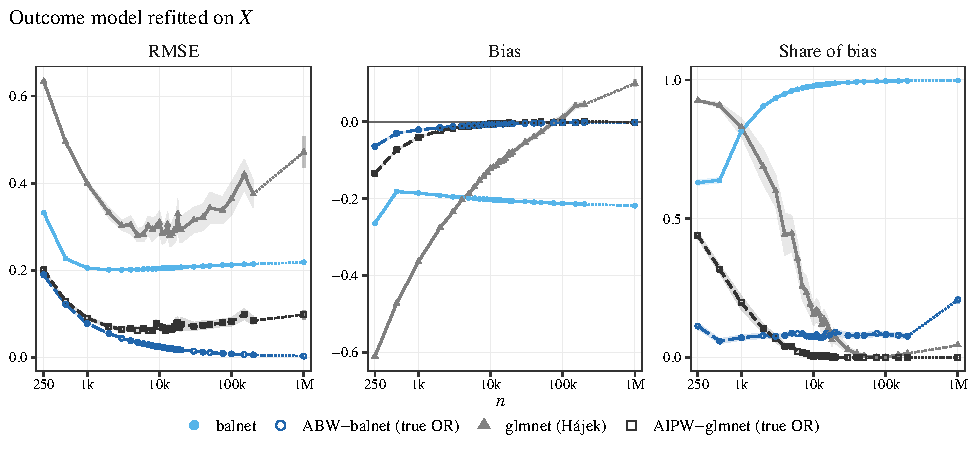
\includegraphics[keepaspectratio]{AAAAA-Working-Thesis_files/figure-pdf/fig-n-refit-1.pdf}}

}

\caption{\label{fig-n-refit}Outcome model refitted on \(X\) by \(n\),
misspecified propensity score, linear outcome. \(n\) = 1M (dotted) is a
separate run.}

\end{figure}%

Once both models are fitted on the observed \(\tilde X\), the double
fragility of AIPW is clear. The outcome model that protected it in the
refit is now a second source of error. Fitted on \(\tilde X\), it leaves
the part of the outcome missed by its linear covariates in its
residuals, which are then weighted by the misspecified MLE weights, so
the bias is the imbalance those weights leave in the residual
(Ben-Michael et al. 2021).

Figure~\ref{fig-n-misspec} follows \texttt{balnet}\(_{10^{-4}}\) and the
modelling estimators across our three doubly wrong settings. Our
balancing estimator converges, but to the wrong value, as is expected of
a misspecified estimator. Its variance shrinks towards zero and its bias
settles near \(-0.22\), \(-0.07\) and \(-0.14\) under the linear,
quadratic and exponential outcome functions
(Appendix Table~\ref{atbl-n-path}). We focus on the Hájek and AIPW
estimators, as the poor performance of the HT estimator is well
documented (Kang and Schafer 2007; Busso et al. 2014), and leave its
results to the appendix.

\begin{figure}

\centering{

\pandocbounded{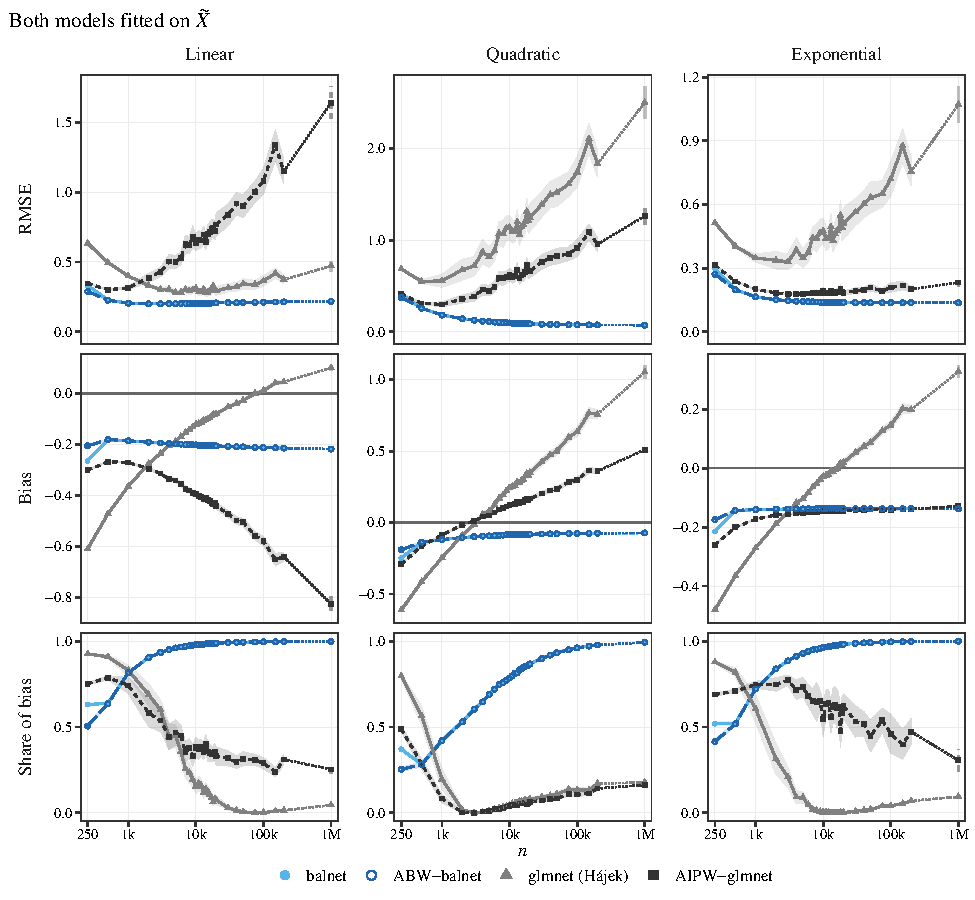
\includegraphics[keepaspectratio]{AAAAA-Working-Thesis_files/figure-pdf/fig-n-misspec-1.pdf}}

}

\caption{\label{fig-n-misspec}Both models fitted on \(\tilde X\) by
\(n\), misspecified propensity score. \(n\) = 1M (dotted) is a separate
run. ABW coincides with balnet from \(n\) = 500.}

\end{figure}%

The Hájek estimator does not settle. Under every outcome function its
bias shrinks through zero and then grows positive, and its RMSE passes a
minimum and rises to the largest sample. More data makes it worse, a
direction Testa et al. (2026) also saw to \(n = 1000\). Kang and Schafer
(2007) traced the worsening to a few enormous weights where the fitted
model misses in the region of near-zero scores. As \(n\) grows those
tails lengthen rather than settling, and the share of the sample
carrying the weight shrinks with it. At \(n = 500\) the MLE weights are
no more extreme than the true score's, with a similar largest weight and
a larger effective sample size
(Appendix Table~\ref{atbl-app-n-diag-m-lin}), so the tails cannot
explain the bias. Here, the bias comes from the imbalance the weights
leave in \(\tilde X\).

Under the linear outcome function the balancing weights settle at the
same bias alone and augmented, near \(-0.2\), well below the Hájek
estimator. Augmented, they reduce to OLS on \(\tilde X\), as exact
balance makes the outcome model a linear adjustment on \(\tilde X\)
(Bruns-Smith et al. 2026). Unaugmented, they differ from that OLS only
by the approximation error, so both carry the part of the outcome not
linear in \(\tilde X\). The double fragility of AIPW is pronounced here.
Its path starts ahead of the Hájek estimator, slips behind it by
\(n = 2000\), and loses ground from there to over three times its RMSE
by \(n = 10^6\) (Appendix Table~\ref{atbl-n-path}). This is the ordering
Kang and Schafer (2007) report up to \(n = 1000\), here holding to
\(10^6\). For AIPW, two wrong models have previously been found to beat
one when the outcome model's misspecification is moderate, though every
bias still scales with the propensity score error (Waernbaum and
Pazzagli 2023). Here the two errors compound instead.

Under the quadratic and exponential outcome functions the outcome model
is also wrong in form, yet AIPW now beats the Hájek estimator, likely
because the linear model in \(\tilde X\) picks up part of the outcome's
curvature, so its residual is less imbalanced than the outcome itself
(Ben-Michael et al. 2021). It still stays well behind ABW, and
\texttt{balnet}\(_{10^{-4}}\) pulls further ahead of the Hájek
estimator. Under the exponential, AIPW is the one modelling series that
settles, at a bias near \(-0.13\). The outcome's \(\exp(X_1/2)\) term is
linear in \(\tilde X_1\), so the outcome model may fit exactly the part
of the outcome where most of the score's signal sits. Refitting the
outcome model on \(X\) does not rescue AIPW under either outcome
function, and under the quadratic it makes both augmented estimators
worse at large \(n\). The same wrong-form model costs almost nothing
under a correctly specified propensity score, where both augmented
estimators are nearly unbiased, so what AIPW appears unable to carry is
the pairing of two wrong models.

Misspecification costs the balancing weights a fixed bias that more data
does not shrink. For modelling, it costs the weights a bias that falls,
crosses zero and grows again while their tails lengthen with \(n\), and
that bias compounds in AIPW under the linear outcome function. Balancing
stays ahead at every \(n\) under every outcome function, alone and
augmented, and the bias of \texttt{cv.glmnet} has not settled by
\(n = 10^6\).

\subsection{Overlap}\label{sec-s1-overlap}

Pooled over overlap and both specifications, balancing estimators have
lower RMSE on average, and \texttt{balnet}\(_{10^{-4}}\) has lower RMSE
than the Hájek estimator in every cell (Table~\ref{tbl-ov-adv}). ABW has
on average \(20.2\%\) lower RMSE than \texttt{balnet}\(_{10^{-4}}\) and
\(32.5\%\) lower than AIPW, while the unaugmented \texttt{balnet} has on
average \(23.1\%\) lower than AIPW and \(59.9\%\) lower than the Hájek
estimator.

\begin{table}[!htbp]

\caption{\label{tbl-ov-adv}\(\bar R(\Theta)\) and \(\bar s_m(\Theta)\)
of A against B, \(c\) = 0.05 to 2, \(n\) = 1000 and 10 000, both
specifications.}

\centering{

\fontsize{8.0pt}{10.0pt}\selectfont
\begin{tabular*}{\linewidth}{@{\extracolsep{\fill}}llrrrrrr}
\toprule
 &  & \multicolumn{4}{c}{{\(\bar R(\Theta)\)}} & \multicolumn{2}{c}{{\(\bar s_m(\Theta)\)}} \\ 
\cmidrule(lr){3-6} \cmidrule(lr){7-8}
Estimator (A) & Comparator (B) & All & Linear & Quadratic & Exponential & \(m = A\) & \(m = B\) \\ 
\midrule\addlinespace[2.5pt]
balnet & AIPW-glmnet & 23.1 & 22.0 & 35.5 & 9.6 & 0.55 & 0.34 \\ 
 & glmnet (Hájek) & 59.9 & 57.2 & 64.7 & 57.5 & 0.55 & 0.67 \\ 
{ABW-balnet} & {balnet} & {20.2} & {21.6} & {20.1} & {19.0} & {0.44} & {0.58} \\ 
 & AIPW-glmnet & 32.5 & 32.4 & 43.4 & 19.6 & 0.46 & 0.34 \\ 
\bottomrule
\end{tabular*}
\begin{minipage}{\linewidth}
\vspace{.05em}
Largest MCSE: 0.4 points (\(\bar R(\Theta)\)), 0.004 (\(\bar s_m(\Theta)\)). The averages are over 84 cells, 42 per specification, at 10 000 Monte Carlo replications. Pairs with glmnet omit the six correct-specification cells at \(c\) = 0.05, where glmnet lacks more than 1\% of its estimates.\\
\end{minipage}

}

\end{table}%

AIPW has lower RMSE than \texttt{balnet}\(_{10^{-4}}\) on average only
where common support is practically violated and the propensity score is
correctly specified. There MLE's performance is also unobservable at
\(c = 0.05\), where \(81.8\%\) of the sample have a propensity score
below \(0.01\) or above \(0.99\) (Appendix Table~\ref{atbl-ov-levels}).

Where we assume common support holds, both balancing estimators have
lower RMSE on average than the modelling estimators, with ABW averaging
\(7.5\%\) lower RMSE than AIPW and \(0.2\%\) lower than
\texttt{balnet}\(_{10^{-4}}\) across outcome functions
(Table~\ref{tbl-ov-adv-hi}). Balancing's advantage here holds across
nonlinear outcomes, though for the linear outcome function, where the
shared outcome model is correct, ABW has \(0.6\%\) higher RMSE than AIPW
while \texttt{balnet}\(_{10^{-4}}\) has \(0.8\%\) higher. For
misspecified propensity scores, both balancing estimators have RMSE
around \(51\%\) lower than AIPW, as on the sample-size grid.

\begin{table}[!htbp]

\caption{\label{tbl-ov-adv-hi}\(\bar R(\Theta)\) and
\(\bar s_m(\Theta)\) of A against B where common support holds.}

\centering{

\fontsize{8.0pt}{10.0pt}\selectfont
\begin{tabular*}{\linewidth}{@{\extracolsep{\fill}}llrrrrrr}
\toprule
 &  & \multicolumn{4}{c}{{\(\bar R(\Theta)\)}} & \multicolumn{2}{c}{{\(\bar s_m(\Theta)\)}} \\ 
\cmidrule(lr){3-6} \cmidrule(lr){7-8}
Estimator (A) & Comparator (B) & All & Linear & Quadratic & Exponential & A & B \\ 
\midrule\addlinespace[2.5pt]
\multicolumn{8}{l}{{\bfseries Correct specification}} \\[2.5pt] 
\midrule\addlinespace[2.5pt]
balnet & AIPW-glmnet & 7.2 & -0.8 & 15.8 & 6.0 & 0.02 & 0.08 \\ 
{ABW-balnet} & {balnet} & {0.2} & {0.2} & {0.3} & {0.2} & {0.02} & {0.02} \\ 
 & AIPW-glmnet & 7.5 & -0.6 & 16.1 & 6.2 & 0.02 & 0.08 \\ 
\midrule\addlinespace[2.5pt]
\multicolumn{8}{l}{{\bfseries Misspecified propensity score}} \\[2.5pt] 
\midrule\addlinespace[2.5pt]
{balnet} & {AIPW-glmnet} & {51.3} & {53.8} & {65.9} & {26.8} & {0.76} & {0.46} \\ 
{ABW-balnet} & {AIPW-glmnet} & {51.4} & {53.9} & {66.0} & {27.0} & {0.76} & {0.46} \\ 
\bottomrule
\end{tabular*}
\begin{minipage}{\linewidth}
\vspace{.05em}
Largest MCSE: 0.7 points (\(\bar R(\Theta)\)), 0.008 (\(\bar s_m(\Theta)\)). Overlap \(c\) = 0.5 to 2 at \(n\) = 1000 and 10 000. The averages are over 24 cells per specification, at 10 000 Monte Carlo replications.\\
\end{minipage}

}

\end{table}%

Where we assume common support is violated, under a correctly specified
score ABW has \(21.7\%\) lower RMSE than AIPW while the unaugmented
\texttt{balnet} has around \(1.5\) times the RMSE of AIPW
(Table~\ref{tbl-ov-adv-lo}). This ordering holds under every outcome
function, with the gap to \texttt{balnet}\(_{10^{-4}}\) widest under the
linear outcome. Under a misspecified score, for all \(c \leq 0.25\) ABW
has \(37.7\%\) lower RMSE than AIPW on average, while
\texttt{balnet}\(_{10^{-4}}\) has \(29.3\%\) lower. As in simulations
with practical or outright positivity violations,
\texttt{balnet}\(_{10^{-4}}\) has lower RMSE than the Hájek estimator
(Chattopadhyay et al. 2020; Keele et al. 2026) but is biased where its
path truncates. Under a misspecified score the lowest RMSE at the
weakest overlap does not improve with \(n\)
(Appendix Table~\ref{atbl-app-ov-full-m}).

\begin{table}[!htbp]

\caption{\label{tbl-ov-adv-lo}\(\bar R(\Theta)\) and
\(\bar s_m(\Theta)\) of A against B where common support is violated.}

\centering{

\fontsize{8.0pt}{10.0pt}\selectfont
\begin{tabular*}{\linewidth}{@{\extracolsep{\fill}}llrrrrrr}
\toprule
 &  & \multicolumn{4}{c}{{\(\bar R(\Theta)\)}} & \multicolumn{2}{c}{{\(\bar s_m(\Theta)\)}} \\ 
\cmidrule(lr){3-6} \cmidrule(lr){7-8}
Estimator (A) & Comparator (B) & All & Linear & Quadratic & Exponential & A & B \\ 
\midrule\addlinespace[2.5pt]
\multicolumn{8}{l}{{\bfseries Correct specification}} \\[2.5pt] 
\midrule\addlinespace[2.5pt]
balnet & AIPW-glmnet & -49.6 & -77.5 & -27.6 & -47.8 & 0.65 & 0.18 \\ 
{ABW-balnet} & {AIPW-glmnet} & {21.7} & {12.7} & {30.5} & {20.9} & {0.13} & {0.18} \\ 
\midrule\addlinespace[2.5pt]
\multicolumn{8}{l}{{\bfseries Misspecified propensity score}} \\[2.5pt] 
\midrule\addlinespace[2.5pt]
{balnet} & {AIPW-glmnet} & {29.3} & {35.6} & {33.0} & {17.9} & {0.90} & {0.62} \\ 
{ABW-balnet} & {AIPW-glmnet} & {37.7} & {44.2} & {42.3} & {24.8} & {0.87} & {0.62} \\ 
\bottomrule
\end{tabular*}
\begin{minipage}{\linewidth}
\vspace{.05em}
Largest MCSE: 2.0 points (\(\bar R(\Theta)\)), 0.004 (\(\bar s_m(\Theta)\)). Overlap \(c\) = 0.05 to 0.25 at \(n\) = 1000 and 10 000. The averages are over 12 cells under correct specification and 18 under misspecification, at 10 000 Monte Carlo replications.\\
\end{minipage}

}

\end{table}%

As overlap degrades below \(c = 0.5\), the share of bias rises for both
balancing estimators. Under correct specification, averaged over both
sample sizes, the unaugmented \texttt{balnet} jumps from a \(1\%\) share
at \(c = 0.5\) to \(41\%\) at \(c = 0.25\) under linear outcomes
(Figure~\ref{fig-ov-adv}). This average hides a split by sample size,
with the share \(83\%\) at \(n = 1000\), where every path stops short,
and zero at \(n = 10{,}000\), where nearly every path reaches its target
(Appendix Table~\ref{atbl-app-ov-full-c}). In contrast, ABW moves from
unbiased to a \(6\%\) share, rising to \(28\%\) by \(c = 0.05\) where
\texttt{balnet}\(_{10^{-4}}\) is at \(97\%\). This pattern holds across
outcomes, except that ABW under quadratic outcomes becomes more variance
driven on either side of \(c = 0.25\).

\begin{figure}

\centering{

\pandocbounded{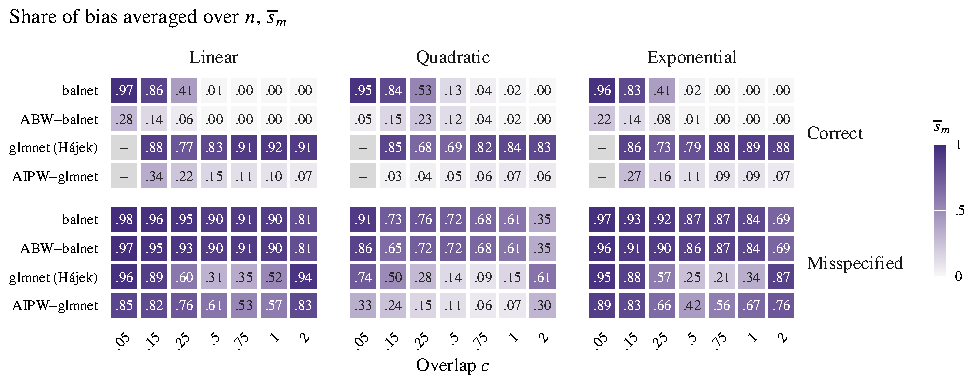
\includegraphics[keepaspectratio]{AAAAA-Working-Thesis_files/figure-pdf/fig-ov-adv-1.pdf}}

}

\caption{\label{fig-ov-adv}Share of bias by \(c\), averaged over \(n\) =
1000 and 10 000, both specifications. glmnet (HT) not drawn. Grey cells
are left out for missing estimates.}

\end{figure}%

Appendix Figure~\ref{afig-app-nc} follows the estimators as overlap
improves in small and large samples. Across all settings, ABW has lower
RMSE than the unaugmented \texttt{balnet} wherever the path of
\texttt{balnet} stops short of exact balance, increasingly so under a
correctly specified score as overlap degrades, and with more data the
path reaches exact balance at poorer overlap.

Where we assume common support holds, ABW has the lowest RMSE of the
modelling and balancing estimators in small samples under every outcome.
In these samples AIPW also has a lower RMSE than
\texttt{balnet}\(_{10^{-4}}\) under a correctly specified score, and
this extends to larger samples as overlap degrades. Under a misspecified
propensity score the advantage of \texttt{balnet}\(_{10^{-4}}\) over
AIPW extends to poorer overlap, with a lower RMSE at \(n = 5000\) from
\(c = 0.1\), even where its path truncates, and at every \(c\) under
linear outcomes.

Where we assume common support is practically violated,
\texttt{balnet}\(_{10^{-4}}\) truncates at every \(n\), with a higher
RMSE than ABW in both samples, far more so under a correctly specified
score. Under a misspecified score AIPW has a lower RMSE than ABW at the
weakest overlap under the quadratic outcome and the two are level under
the exponential, but as overlap improves ABW takes over, earlier in the
larger sample, consistent with approximate residual balancing
outperforming AIPW in the misspecified setting of Athey et al. (2018),
which varied dimension. At the weakest overlap no weighting estimator
removes half the confounding in either sample, as in Keele et al.
(2026), where no method overcame outcome misspecification once overlap
was poor.\footnote{At \(c = 0.01\) the unadjusted difference is
  \(-2.06\) (linear, quadratic) and \(-1.56\) (exponential) at both
  \(n\), against a lowest weighting RMSE of \(1.08\) (design values,
  weighting RMSEs in Appendix Table~\ref{atbl-app-nc-full-m}).}

\subsection{High-dimensional settings}\label{sec-s1-hd}

\begin{table}[!htbp]

\caption{\label{tbl-pn-adv}\(\bar R(\Theta)\) of A against B and
\(\bar s_m(\Theta)\) of A over all \(p/n\), at exact balance and once
the path stops short, \(n\) = 500 and 1000.}

\centering{

\fontsize{8.0pt}{10.0pt}\selectfont
\begin{tabular*}{\linewidth}{@{\extracolsep{\fill}}llrrrrr}
\toprule
 &  & \multicolumn{3}{c}{{\(\bar R(\Theta)\)}} & \multicolumn{2}{c}{{\(\bar s_m(\Theta)\), \(m = A\)}} \\ 
\cmidrule(lr){3-5} \cmidrule(lr){6-7}
Estimator (A) & Comparator (B) & All & Exact balance & Path truncates & Exact balance & Path truncates \\ 
\midrule\addlinespace[2.5pt]
\multicolumn{7}{l}{{\bfseries Correct specification}} \\[2.5pt] 
\midrule\addlinespace[2.5pt]
balnet & glmnet (Hájek) & 49.1 & 66.9 & 36.9 & 0.01 & 0.89 \\ 
 & AIPW-glmnet & -48.0 & 3.0 & -82.8 & 0.01 & 0.89 \\ 
{ABW-balnet} & {balnet} & {41.6} & {0.0} & {55.4} & {0.01} & {0.46} \\ 
 & AIPW-glmnet & 13.6 & 3.0 & 18.4 & 0.01 & 0.46 \\ 
\midrule\addlinespace[2.5pt]
\multicolumn{7}{l}{{\bfseries Misspecified propensity score}} \\[2.5pt] 
\midrule\addlinespace[2.5pt]
{balnet} & {glmnet (Hájek)} & {39.2} & {55.5} & {28.9} & {0.57} & {0.89} \\ 
 & AIPW-glmnet & -7.9 & 25.4 & -29.8 & 0.57 & 0.89 \\ 
{ABW-balnet} & {balnet} & {23.8} & {0.2} & {33.5} & {0.57} & {0.75} \\ 
 & AIPW-glmnet & 17.8 & 25.5 & 13.7 & 0.57 & 0.75 \\ 
\bottomrule
\end{tabular*}
\begin{minipage}{\linewidth}
\vspace{.05em}
Cells per specification: 36 in all, 12 while exact balance holds and 24 once the path truncates, at 10 000 Monte Carlo replications. Largest MCSE: 0.8 points (\(\bar R(\Theta)\)), 0.019 (\(\bar s_m(\Theta)\)).\\
\end{minipage}

}

\end{table}%

As covariates are added, balancing keeps its advantage over modelling on
average, alone and augmented (Table~\ref{tbl-pn-adv}).
\texttt{balnet}\(_{10^{-4}}\) has lower RMSE than \texttt{cv.glmnet}
(Hájek) in every cell, by \(49.1\%\) on average under a correctly
specified score and \(39.2\%\) under misspecification. Augmentation
narrows this to \(13.6\%\) and \(17.8\%\) for ABW over AIPW, and on
average AIPW overtakes the unaugmented \texttt{balnet}.

These averages hide the expected change at \(p/n = 0.5\), from which
every \texttt{balnet}\(_{10^{-4}}\) path stops short of exact balance.
Bias then makes up most of its error, with its share rising from
\(0.01\) to \(0.89\) under a correctly specified score
(Table~\ref{tbl-pn-adv}). Here, its lead over the Hájek estimator nearly
halves, from \(66.9\%\) to \(36.9\%\), and it also slips behind the
oracle (Appendix Table~\ref{atbl-app-pn-full-c}).

ABW again collapses to \texttt{balnet}\(_{10^{-4}}\) at exact balance.
Once the path stops short, the outcome model adjusts for the remaining
imbalance, and ABW's RMSE is \(55.4\%\) and \(33.5\%\) lower than that
of \texttt{balnet}\(_{10^{-4}}\). Unlike \texttt{balnet}\(_{10^{-4}}\),
ABW stays ahead of AIPW, by \(18.4\%\) and \(13.7\%\). Its lead widens
from \(p/n = 0.5\) under a correctly specified score but narrows under
misspecification.

Once the path stops short, the lead of \texttt{balnet}\(_{10^{-4}}\)
over the Hájek estimator narrows as \(p\) grows under all settings
(Figure~\ref{fig-pn-rmse}). Both estimators grow more biased, but at
different rates. As expected, the bias of the Hájek estimator grows
gradually, while that of \texttt{balnet}\(_{10^{-4}}\) grows faster as
its leftover imbalance increases with \(p\) (Zhao 2019). Its nonzero
coefficients stop growing with \(p\) once the path stops short
(Appendix Table~\ref{atbl-app-pn-diag-c-lin};
Appendix Table~\ref{atbl-app-pn-diag-m-lin}). Our grid extends the
comparison of Tan (2020b) to higher dimensions, up to \(p/n = 4\), where
the narrowing we find between the unaugmented estimators mirrors the
result of Athey et al. (2018) for approximately balancing weights.

\begin{figure}

\centering{

\pandocbounded{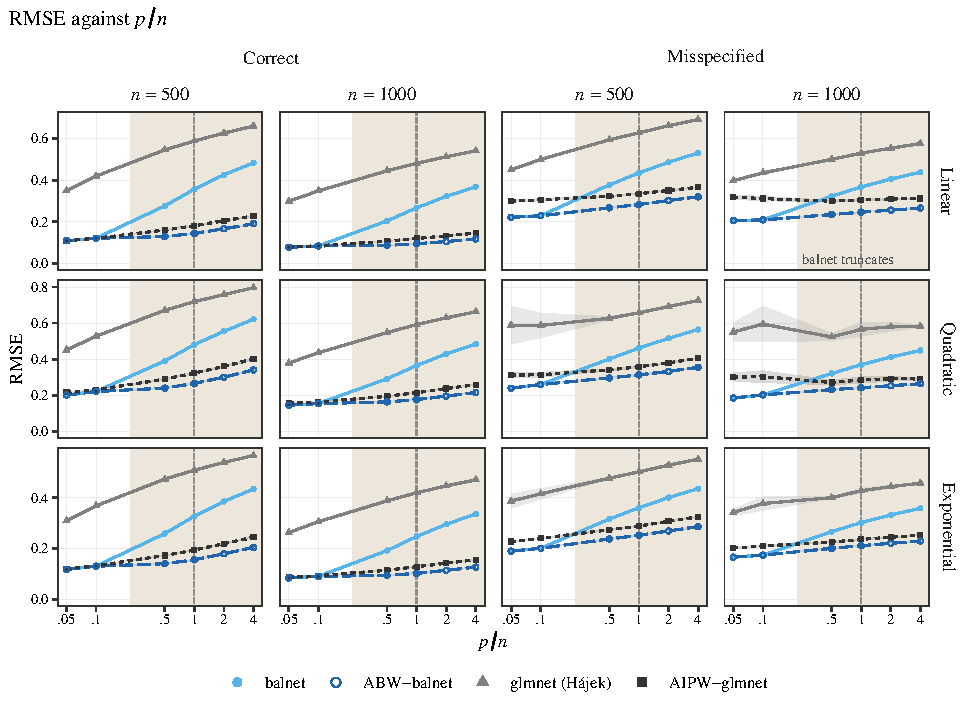
\includegraphics[keepaspectratio]{AAAAA-Working-Thesis_files/figure-pdf/fig-pn-rmse-1.pdf}}

}

\caption{\label{fig-pn-rmse}RMSE against \(p/n\) at \(n\) = 500 and
1000, both specifications. Shading marks where the balnet path stops
short, the dotted line \(p = n\).}

\end{figure}%

Augmentation does not remove the whole cost of the leftover imbalance,
with ABW's bias still growing with \(p\) from \(p/n = 0.5\)
(Appendix Figure~\ref{afig-app-pn-bias}). Its lead over AIPW holds
steady at \(15\%\) to \(21\%\) under a correctly specified score
(Appendix Table~\ref{atbl-app-pn-full-c}), but narrows as \(p\) grows
under misspecification, most clearly for the linear outcome. The
narrowing comes from both sides, as ABW's bias grows faster than AIPW's
once the path stops short, while AIPW's variance falls with \(p\) and
offsets its own growing bias, most of all at \(n = 1000\). To our
knowledge this narrowing has not been reported, and the augmented
balancing weights of Athey et al. (2018), which target balance without a
propensity score, show a steady lead over AIPW.\footnote{Unlike ours,
  their AIPW used elastic-net propensity scores trimmed at 0.05 and 0.95
  (Athey et al. 2018).}

The cost of misspecification to the MLE estimators shrinks as covariates
are added. For the Hájek estimator this cost falls in every series, and
has vanished or reversed for nonlinear outcomes by \(p/n = 4\). Though
the relative cost falls, Hájek's RMSE still generally rises with \(p\),
consistent with the findings of Athey et al. (2018). As discussed
earlier, misspecification costs AIPW more than the Hájek estimator at
low \(p\), and this cost too shrinks as \(p\) grows
(Figure~\ref{fig-pn-rmse}).

\textbf{With a denser covariate profile:} With four confounders,
\(\nu = 1\) and independent covariates, the sparsity grid shares the
propensity score of the \(p/n\) grid. From \(p/n = 0.5\) every
\texttt{balnet} path stops short of exact balance, whatever \(s\),
\(\nu\) or \(\rho\), so exact balance and the truncated path are
reported apart throughout (Figure~\ref{fig-sp-change}). \texttt{balnet}
again has lower RMSE than the Hájek estimator in every cell under both
scores, and by more than three MCSE in all but one under Tan's
transformation, whatever the number of confounders, their decay or the
covariate correlation.\footnote{In the remaining cell (\(n = 1000\),
  \(s = 4\), \(\nu = 1\), AR(1), quadratic outcome) the RMSE of
  \texttt{balnet} is \(40\%\) of the Hájek estimator's, but heavy-tailed
  Hájek estimates leave the ratio within three MCSE of one, so it is not
  counted as a win.} ABW keeps a lead over AIPW on average under
independent and AR(1)-correlated covariates, but under equicorrelation
the two stay within a few per cent.

\begin{figure}

\centering{

\pandocbounded{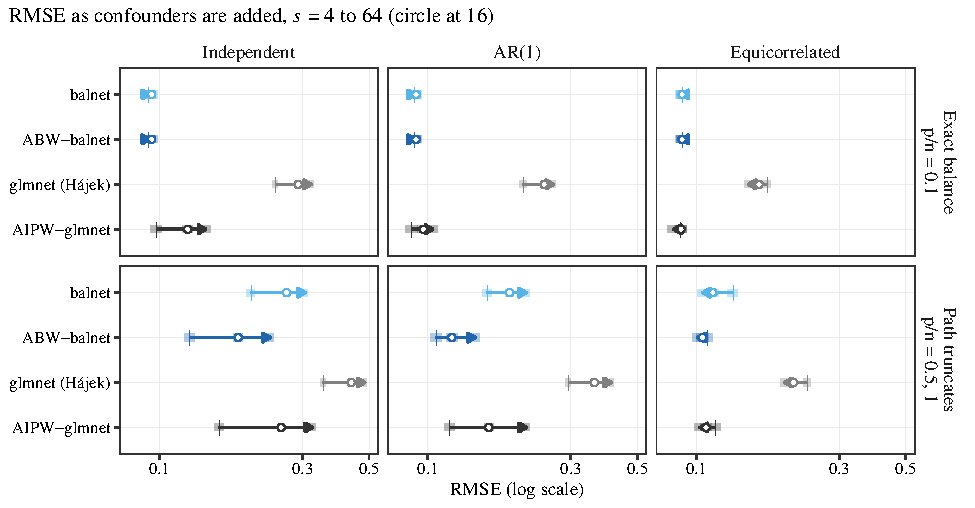
\includegraphics[keepaspectratio]{AAAAA-Working-Thesis_files/figure-pdf/fig-sp-change-1.pdf}}

}

\caption{\label{fig-sp-change}RMSE by \(s\) and covariance structure,
correct specification, at exact balance and once the path stops short,
pooled over outcomes and decay rates. glmnet (HT) not drawn.}

\end{figure}%

\textbf{Dynamics across} \(s\): While exact balance holds,
\texttt{balnet} stays close to unbiased in every cell, with absolute
bias at most 0.006 for the linear outcome and 0.028 for the quadratic,
at every \(s\), \(\nu\) and \(\rho\)
(Appendix Table~\ref{atbl-app-sp-cells}). Here, the Hájek estimator
grows more biased as confounders are added under independent and
AR(1)-correlated covariates, so the lead of \texttt{balnet} widens with
\(s\), from \(62.2\%\) to \(71.1\%\) under independent and from
\(56.5\%\) to \(65.3\%\) under AR(1)-correlated covariates at
\(n = 1000\). The lead is larger under slower decay, whereas under
equicorrelation it narrows instead
(Appendix Table~\ref{atbl-app-sp-exact}). As expected, the error of the
MLE weights grows with the number of active covariates (Tan 2020a).
Exact balance instead removes the bias for the linear outcome at any
\(s\).

Once the path stops short, all four estimators are biased downwards
(Appendix Table~\ref{atbl-app-sp-cells}). The bias of \texttt{balnet}
grows as confounders are added and, beyond four, as their decay slows,
and is smaller under AR(1)-correlated covariates, consistent with the
findings of Zhao (2019) for the number of confounders and of Athey et
al. (2018) for correlation. Under equicorrelation it falls with \(s\)
instead. \texttt{balnet} still keeps a lead of \(37\%\) to \(48\%\) over
the Hájek estimator at every \(s\), though its error turns to bias, with
a share rising from 0.73 to 0.86 under independent and from 0.60 to 0.76
under AR(1)-correlated covariates
(Appendix Table~\ref{atbl-app-sp-trunc}). Its linear bias is nearly the
full imbalance bound with four confounders but between a half and three
quarters of it with 64 under independent and AR(1)-correlated covariates
(Appendix Table~\ref{atbl-app-sp-bound}).

The gain from augmentation follows the same split. Once the path stops
short, ABW has lower RMSE than AIPW in every cell under independent and
AR(1)-correlated covariates, and its lead grows with \(s\), from
\(20.1\%\) to \(28\%\) by 16 confounders under independent and from
\(10.0\%\) to \(32.5\%\) under AR(1)-correlated covariates
(Appendix Table~\ref{atbl-app-sp-trunc}). Under these two structures
both augmented estimators grow more biased as confounders are added,
AIPW faster. As expected, AIPW loses ground as the propensity model it
relies on grows denser (Athey et al. 2018). This is consistent with the
findings of Bradic et al. (2019), where the error of AIPW rose with the
number of active propensity covariates while that of augmented balancing
weights did not. While exact balance holds, the same pattern appears at
\(n = 1000\), from a lead of \(5.8\%\) under independent and none under
AR(1)-correlated covariates at four confounders to \(35.0\%\) and
\(12.5\%\) at 64.

The unaugmented \texttt{balnet} also catches AIPW as confounders are
added. Once the path stops short, \texttt{balnet} has 1.3 times the RMSE
of AIPW at four confounders under independent and AR(1)-correlated
covariates. At 64 it is level with AIPW under AR(1)-correlated
covariates and ahead under independent ones, and the gap shrinks with
\(s\) under every covariance structure
(Appendix Table~\ref{atbl-app-sp-trunc}). Here, the bias of AIPW grows
with \(s\) faster than that of \texttt{balnet}, while under
equicorrelation the bias of \texttt{balnet} falls faster.

Tan's transformation costs \texttt{balnet}, not the Hájek estimator, and
only while exact balance holds. There the RMSE of \texttt{balnet} rises
by about a half under independent covariates, two thirds for the linear
outcome, and by a fifth under AR(1), so the lead narrows from \(63.6\%\)
to \(49.6\%\) under independent covariates and little elsewhere
(Appendix Table~\ref{atbl-app-sp-tan}). Here, exact balance on the
transformed covariates does not guarantee balance in the original ones,
in which the outcome is linear, so part of the confounding bias can
return (Zhao 2019). This differs from the findings of Tan (2020b), where
balancing weights had similar or smaller MSE under a correct score and a
substantial advantage under a Kang--Schafer misspecification. Under the
transformation the lead of ABW over AIPW also narrows with \(s\) at
exact balance, the reverse of its direction under a correct score. The
direction matches the findings of Tan (2020a) under a misspecified
score, though their outcome model was correct.

Equicorrelated covariates break the pattern. While exact balance holds,
the Hájek estimator grows less biased as confounders are added, so the
lead of \texttt{balnet} narrows from \(47.7\%\) to \(40.4\%\) instead of
widening, and once the path stops short the bias of \texttt{balnet}
falls with \(s\) too (Appendix Table~\ref{atbl-app-sp-exact};
Appendix Table~\ref{atbl-app-sp-trunc}). ABW and AIPW stay within a few
per cent of each other at exact balance and once the path stops short,
and Tan's transformation costs \texttt{balnet} little. We read this
through \(Z_0\), the common factor every equicorrelated covariate
shares, which makes up about three quarters of the variance of the
propensity index at four confounders and over nine tenths at 64
(Appendix Table~\ref{atbl-app-sp-share}). Here, a sparse fit already
captures most of the confounding, so balancing more columns adds little.

\subsection{Outcome signal}\label{sec-s1-signal}

Under a correctly specified propensity score, the ranking of
\texttt{balnet}\(_{10^{-4}}\) and the Hájek estimator reverses as the
outcome signal grows against the fixed noise
(Appendix Table~\ref{atbl-app-sig-full-c}). As only the ratio of signal
to noise decides the ranking, a low \(\kappa\) reads as a noisy outcome.
In the noisiest cells, \(\kappa \le 0.05\),
\texttt{balnet}\(_{10^{-4}}\) has \(9\%\) to \(12\%\) higher RMSE, and
once the noise falls back, from \(\kappa = 0.2\), it has lower RMSE, by
\(62\%\) to \(74\%\) at \(\kappa = 1\). Here, the bias of the Hájek
estimator grows with the signal while \texttt{balnet}\(_{10^{-4}}\)
stays close to unbiased, but exact balance leaves it a smaller effective
sample size (median 345 against 430 per arm,
Appendix Table~\ref{atbl-app-sig-diag-c-lin}), which decides the ranking
while the noise dominates. Its \(32.9\%\) advantage pooled over
\(\kappa\) (Table~\ref{tbl-sig-adv}) averages over the cells where its
RMSE is higher. The oracle reverses against
\texttt{balnet}\(_{10^{-4}}\) in the same way, so the efficiency
advantage of exact balance holds only once the signal clears the noise.

\begin{table}[!htbp]

\caption{\label{tbl-sig-adv}\(\bar R(\Theta)\) and \(\bar s_m(\Theta)\)
of balnet against glmnet (Hájek), correct specification, \(\kappa\) =
0.02 to 1.}

\centering{

\fontsize{8.0pt}{10.0pt}\selectfont
\begin{tabular*}{\linewidth}{@{\extracolsep{\fill}}llrrrrrr}
\toprule
 &  & \multicolumn{4}{c}{{\(\bar R(\Theta)\)}} & \multicolumn{2}{c}{{\(\bar s_m(\Theta)\)}} \\ 
\cmidrule(lr){3-6} \cmidrule(lr){7-8}
Estimator (A) & Comparator (B) & All & Linear & Quadratic & Exponential & \(m = A\) & \(m = B\) \\ 
\midrule\addlinespace[2.5pt]
balnet & glmnet (Hájek) & 32.9 & 35.9 & 32.5 & 30.3 & 0.00 & 0.47 \\ 
\bottomrule
\end{tabular*}
\begin{minipage}{\linewidth}
\vspace{.05em}
Largest MCSE: 0.1 points (\(\bar R(\Theta)\)), 0.002 (\(\bar s_m(\Theta)\)). The averages are over 24 cells at 10 000 Monte Carlo replications.\\
\end{minipage}

}

\end{table}%

Under a misspecified propensity score both estimators are biased in
proportion to the signal, as the bias acts through the outcome (Zhao
2019; Waernbaum and Pazzagli 2023), but the Hájek estimator is about
twice as biased. \texttt{balnet}\(_{10^{-4}}\) has lower RMSE at every
noise level but the highest, by \(49\%\) to \(68\%\) at \(\kappa = 1\),
and the two are level at \(\kappa = 0.02\). There the Hájek estimator
has the lower median absolute error, as a few extreme weights lift its
RMSE.

Augmentation again leaves \texttt{balnet}\(_{10^{-4}}\) unchanged, with
the RMSE of ABW within 0.001 of it in every cell. Under a correctly
specified score the gain for the Hájek estimator grows as the noise
falls, from none at \(\kappa = 0.02\), where the outcome model often
keeps no covariate, to \(59\%\) to \(74\%\) lower RMSE at
\(\kappa = 1\). The augmented pair reverses as the unaugmented one does,
with ABW ahead of AIPW only from \(\kappa = 0.2\), by under \(8\%\).
Under misspecification neither pair reverses, and ABW stays ahead of
AIPW at every noise level but the highest, by \(18\%\) to \(43\%\) at
\(\kappa = 1\).

In a noisy outcome, then, the balance at the end of the \texttt{balnet}
path costs more in variance than it removes in bias, as anticipated
where the best amount of balance depends on the noise relative to the
signal (Zhao 2019).

\subsection{Coverage}\label{sec-s1-coverage}

\begin{figure}

\centering{

\pandocbounded{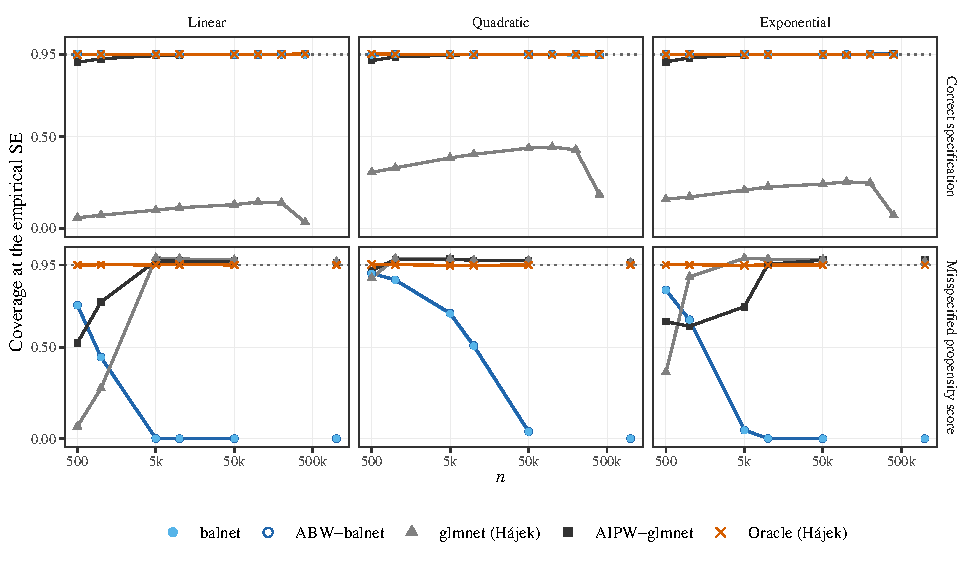
\includegraphics[keepaspectratio]{AAAAA-Working-Thesis_files/figure-pdf/fig-n-coverage-1.pdf}}

}

\caption{\label{fig-n-coverage}Coverage at the empirical SE by \(n\),
both specifications. The dotted line is the nominal 95\%, \(n\) = 1M
(misspecified) a separate run.}

\end{figure}%

Figure~\ref{fig-n-coverage} shows what the biases of Study 1 cost a
confidence interval along \(n\). Under a correctly specified score
\texttt{balnet}\(_{10^{-4}}\), ABW and the oracle sit at nominal at
every \(n\), and AIPW reaches it by \(n = 10{,}000\). The Hájek
estimator never rises above \(0.44\), as the shrinkage bias of its
cross-validated lasso score does not fall with \(n\) while its sampling
error does (share of bias \(0.88\), Table~\ref{tbl-n-adv}). Under
misspecification the picture inverts. The balancing estimators collapse
to zero by \(n = 10{,}000\) for the linear and exponential outcomes and
more slowly for the quadratic, as the intervals zero in on their fixed
bias. The Hájek and AIPW estimators instead reach nominal from
\(n = 5000\), AIPW from \(10{,}000\) under the exponential outcome. In
our design the largest MLE weight grows with \(n\) while the true
score's does not, from a median under ten at \(n = 500\) to several
hundred at \(50{,}000\) (Appendix Table~\ref{atbl-app-n-diag-m-lin}), so
the Hájek and AIPW estimates carry heavy tails that inflate EmpSE beyond
the spread of a typical estimate.

Along overlap, coverage depends on the balance achieved
(Appendix Figure~\ref{afig-ov-coverage}). Under a correctly specified
score \texttt{balnet}\(_{10^{-4}}\) holds nominal coverage where common
support holds and loses it where it is practically violated, AIPW loses
it only at \(c \le 0.15\) under the linear and exponential outcomes, and
ABW stays at or above \(0.83\) at every \(c\). The Hájek estimator sits
below a half at every \(c \ge 0.75\), and at \(c = 0.05\) even the
oracle falls below \(0.15\). Under misspecification the balancing
estimators keep partial coverage at \(n = 1000\), rising with overlap
from near zero at \(c \le 0.15\) to between \(0.7\) and \(0.9\) at
\(c = 2\), before the collapse with \(n\) seen above. The Hájek and AIPW
estimators reach nominal only mid-grid and lose it at both ends, under
practical violations and at \(c = 2\), where the weights are no longer
extreme and their bias is exposed.\footnote{Under misspecification at
  \(n = 10{,}000\) the largest MLE weight in the treated arm has a
  median of \(15\) at \(c = 2\), against \(98\) at \(c = 1\) and about
  \(1450\) at \(c = 0.05\), and the arm's effective sample size is about
  \(4600\) of \(5000\). EmpSE of the Hájek estimator falls to \(0.03\)
  while its bias stays near \(-0.15\) for the linear outcome.}

Noise also obscures bias (Appendix Figure~\ref{afig-sig-coverage}). At
low \(\kappa\) the noise dominates EmpSE and every estimator reaches
nominal coverage. A stronger outcome signal lowers the coverage of a
biased estimator, as its bias grows while EmpSE stays fixed. Under a
correctly specified score both balancing estimators and AIPW hold near
nominal coverage at every \(\kappa\), while the Hájek estimator falls to
between \(0.07\) and \(0.34\) at \(\kappa = 1\). Under misspecification
every estimator is biased and loses coverage as the signal grows, the
balancing estimators to \(0.45\) at \(\kappa = 1\) for the linear
outcome. The quadratic outcome is the exception, where the Hájek and
AIPW estimators stay above nominal. The weights do not depend on the
outcome, so the same tails apply, and under the quadratic outcome they
give the Hájek estimator an EmpSE three times the linear outcome's while
its bias is smaller against it.

Coverage does not change the RMSE orderings above, but illustrates how
the estimators' errors would reach a confidence interval in application.
For the balancing weights it is a fixed bias no variance estimator can
correct, and for the MLE estimators heavy tails can widen the interval
until it includes the true \(\tau\). Where the signal is weak
\texttt{balnet}'s bias is small against EmpSE, so a larger \(\lambda\)
can trade it for variance at little cost to coverage. Study 2 asks where
that RMSE-minimising \(\lambda\) lies inside the path, and whether any
selector finds it.

\section{Study 2 Results}\label{study-2-results}

\subsection{Overview}\label{overview}

Table~\ref{tbl-s2-counts} shows how often the RMSE-minimising
\(\lambda\) comes before the path endpoint and how often a selector
improves on it. As expected, both become more common at weaker outcome
signals, where the endpoint's cost in variance stays fixed by noise
while the bias it removes falls with the signal. With no signal both
estimators have an interior optimum in every cell, in line with Study 1.
From \(\kappa = 1/4\) the two diverge, with \texttt{balnet}'s share
falling from \(35\%\) to \(8\%\) at full signal while ABW's holds near
\(60\%\). On average across our outcome signal levels, an interior
optimum occurs in \(61\%\) of cells for \texttt{balnet} and \(79\%\) for
ABW.

\begin{table}[!htbp]

\caption{\label{tbl-s2-counts}Interior optima and selector wins for
balnet and ABW, (A) by grid, (B) by \(\kappa\).}

\centering{

\fontsize{8.0pt}{10.0pt}\selectfont
\begin{tabular*}{\linewidth}{@{\extracolsep{\fill}}llrrrrrrr}
\toprule
 &  &  & \multicolumn{2}{c}{{Interior optimum (\%)}} & \multicolumn{2}{c}{{Selector win (\%)}} & \multicolumn{2}{c}{{Win given an interior optimum (\%)}} \\ 
\cmidrule(lr){4-5} \cmidrule(lr){6-7} \cmidrule(lr){8-9}
Grid & Factor varied & Cells & balnet & ABW & balnet & ABW & balnet & ABW \\ 
\midrule\addlinespace[2.5pt]
\multicolumn{9}{l}{{\bfseries A. By grid}} \\[2.5pt] 
\midrule\addlinespace[2.5pt]
Overlap & \(c\) & 18 & 0 & 72 & 0 & 67 & – & 92 \\ 
Outcome noise & \(\kappa\) & 21 & 43 & 43 & 38 & 38 & 89 & 89 \\ 
Noise × overlap & \(\kappa\), \(c\) & 84 & 60 & 85 & 57 & 83 & 96 & 99 \\ 
Penalty form × overlap & \(\alpha\), \(c\) & 420 & 58 & 82 & 53 & 80 & 92 & 97 \\ 
Sample size × overlap × penalty & \(n\), \(c\), \(\alpha\) & 336 & 58 & 82 & 57 & 81 & 98 & 99 \\ 
Large \(n\) × overlap & \(n\), \(c\) & 84 & 73 & 100 & 58 & 100 & 80 & 100 \\ 
Dimension × overlap × penalty & \(p\), \(c\), \(\alpha\) & 336 & 68 & 75 & 65 & 73 & 95 & 97 \\ 
Misspecification × overlap & \(c\) & 126 & 53 & 61 & 51 & 62 & 96 & 99 \\ 
Denser profile & \(s\), covariance & 189 & 66 & 79 & 66 & 78 & 98 & 99 \\ 
Denser profile under Tan's transformation & \(s\), covariance & 189 & 66 & 83 & 65 & 81 & 94 & 97 \\ 
{All grids} & {} & {1803} & {61} & {79} & {58} & {78} & {94} & {98} \\ 
\midrule\addlinespace[2.5pt]
\multicolumn{9}{l}{{\bfseries B. By outcome signal \(\kappa\), all grids}} \\[2.5pt] 
\midrule\addlinespace[2.5pt]
\(\kappa\) = 0 &  & 255 & 100 & 100 & 100 & 100 & 100 & 100 \\ 
\(\kappa\) = 1/32 &  & 255 & 99 & 99 & 98 & 98 & 98 & 98 \\ 
\(\kappa\) = 1/16 &  & 255 & 96 & 96 & 92 & 93 & 96 & 97 \\ 
\(\kappa\) = 1/8 &  & 255 & 80 & 82 & 80 & 81 & 99 & 99 \\ 
\(\kappa\) = 1/4 &  & 255 & 35 & 62 & 26 & 60 & 69 & 94 \\ 
\(\kappa\) = 1/2 &  & 255 & 13 & 58 & 9 & 56 & 59 & 97 \\ 
\(\kappa\) = 1 &  & 273 & 8 & 59 & 7 & 60 & 82 & 99 \\ 
\bottomrule
\end{tabular*}
\begin{minipage}{\linewidth}
\vspace{.05em}
Interior optimum: the path minimum is more than 5\% below the endpoint's RMSE. Selector win: a selector's RMSE is below the endpoint's by more than three times their combined MCSE; -- where a grid has no interior optimum. Cells per estimator: design cells × \(\kappa\) levels × three outcomes; pooled rows weight grids by cells. Without an interior optimum a selector won in 9 of 700 cells for balnet and 5 of 373 for ABW. 2500 replications per cell, 1000 at \(n\) = 10 000.\\
\end{minipage}

}

\end{table}%

At least one selector improves on the endpoint in \(58\%\) of cells for
\texttt{balnet} and \(78\%\) for ABW, almost always where an interior
optimum exists. \texttt{cv.bloss} wins most often for both estimators,
followed by \texttt{boot.inf} (Appendix Table~\ref{atbl-s2-selectors}).
Still, none of the five has the lowest RMSE in more than around \(30\%\)
of cells. Applied naively, however, \texttt{boot.inf} appears the
stronger candidate for \texttt{balnet}, with RMSE on average \(5\%\)
below the endpoint's over all settings against \(1\%\) for
\texttt{cv.bloss}. For ABW the two are level on average, at \(15\%\) and
\(16\%\), so \texttt{cv.bloss} remains our choice on its win count.

\subsection{Outcome signal and
overlap}\label{outcome-signal-and-overlap}

\begin{figure}

\centering{

\pandocbounded{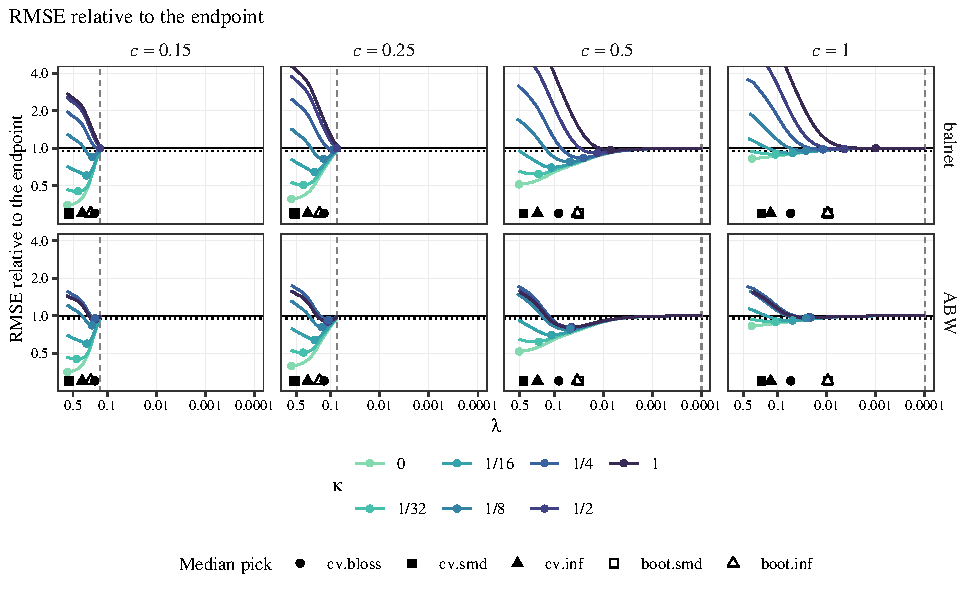
\includegraphics[keepaspectratio]{AAAAA-Working-Thesis_files/figure-pdf/fig-s2-path-1.pdf}}

}

\caption{\label{fig-s2-path}RMSE along the \(\lambda\) path relative to
the endpoint, by \(c\) and \(\kappa\), linear outcome, \(n\) = 1000,
\(p\) = 50. Points mark each minimum, the dotted line the interior rule,
the dashed line the median endpoint \(\lambda\) and symbols each
selector's median \(\lambda\). Ratios above 4 are cut off.}

\end{figure}%

\textbf{Interior optima:} Figure~\ref{fig-s2-path} traces RMSE along the
path relative to the endpoint by overlap and outcome signal. We find
that the outcome signal decides whether \texttt{balnet} has an interior
optimum, while overlap sets how far below the endpoint's RMSE it lies
and how strong a signal it survives. With no signal the path minimum
lies \(65\%\) below the endpoint at \(c = 0.15\) against \(17\%\) at
\(c = 1\), the larger gain under limited overlap we anticipated (Wang
and Zubizarreta 2020). This gain closes as the signal grows, first at
\(c = 1\), where interior optima vanish from \(\kappa = 1/8\), and
everywhere by full signal. Under practical violations of common support,
however, interior optima vanish sooner, lasting to \(\kappa = 1/2\) at
\(c = 0.5\) but not at \(c \le 0.25\). There the path already stops
short of exact balance, so the endpoint weights are already
approximately balanced and a larger \(\lambda\) has little left to gain
for \texttt{balnet}. This suggests \(\lambda\) selection pays most in
between, where the path reaches exact balance but overlap is limited.

For ABW the roles reverse, and overlap rather than signal largely
decides whether an interior optimum exists. At \(c \le 0.5\) it has one
at every signal level, in all but one cell, while at \(c = 1\) its
optima vanish from \(\kappa = 1/8\), as with \texttt{balnet}. Both
estimators share the weights, so a larger \(\lambda\) lowers the
variance of both, and in every interior cell the variance falls at the
path minimum. In an augmented estimator, however, the bias from the
remaining imbalance scales with the error of the outcome model rather
than with the outcome coefficients themselves (Athey et al. 2018). At
full signal the optimal \(\lambda\) of ABW adds only \(13\%\) to
\(16\%\) of the bias it adds to \texttt{balnet} for the linear and
exponential outcomes.\footnote{For the quadratic outcome at full signal
  and \(c \le 0.25\), a larger \(\lambda\) adds no bias to ABW, and at
  \(c = 0.15\) lowers it, since balance on \(X\) does not guarantee
  unbiasedness for an outcome that is not a linear function of \(X\)
  (Zhao 2019).} Here, at \(c \le 0.5\) the variance saved outweighs the
bias added, while at \(c = 1\) there is limited variance to remove.
\(\lambda\) selection for ABW therefore pays wherever overlap is
degraded.

\begin{figure}

\centering{

\pandocbounded{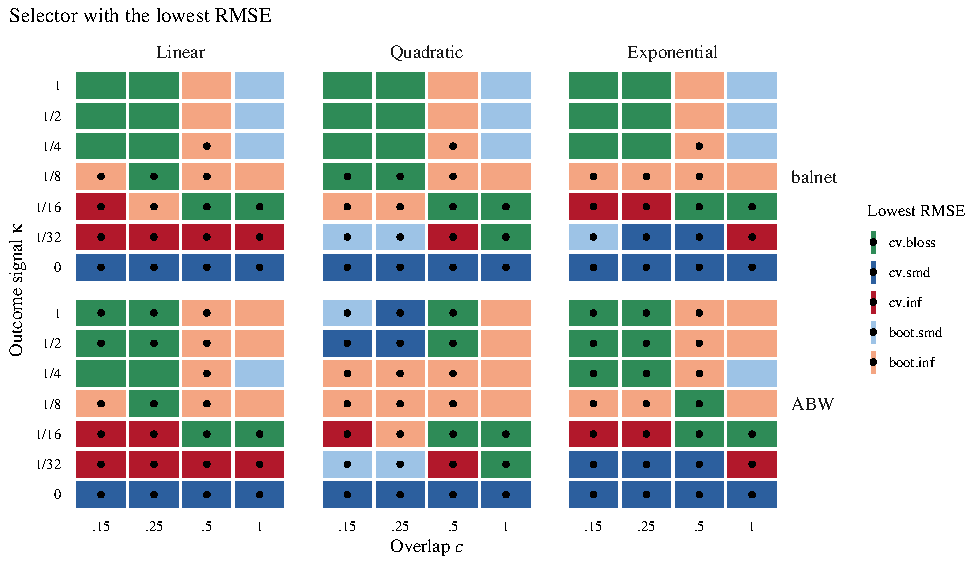
\includegraphics[keepaspectratio]{AAAAA-Working-Thesis_files/figure-pdf/fig-s2-lead-1.pdf}}

}

\caption{\label{fig-s2-lead}Selector with the lowest RMSE per cell by
\(c\) and \(\kappa\), \(n\) = 1000, \(p\) = 50. A dot marks a win
against the endpoint.}

\end{figure}%

\textbf{Selector wins:} Figure~\ref{fig-s2-lead} marks the selector with
the lowest RMSE in each cell and whether it beats the endpoint. At
\(\kappa = 0\) every selector improves on the endpoint of
\texttt{balnet} at \(c \le 0.5\), and \texttt{cv.smd} has the lowest
RMSE in every cell. As the signal grows the lead passes to
\texttt{cv.bloss} and \texttt{boot.inf}, the only two still beating the
untuned estimators in most cells at \(\kappa = 1/8\). By
\(\kappa = 1/4\) only \texttt{boot.inf} wins, in the three cells at
\(c = 0.5\). This is consistent with findings from Tan (2017), where
cross-validating this loss beat unpenalised calibration for pure noise
but lost under the linear outcome we share, as the penalty it keeps
biases the fit along the covariate the outcome loads on most. For
ridge-augmented linear balancing weights, Bruns-Smith et al. (2026)
found cross-validating imbalance the best selector and cross-validating
the balancing loss itself the worst. Here, we find under lasso-penalised
logistic weights the order reverses, with \texttt{cv.bloss} winning in
all nine cells for ABW at full signal and \(c \le 0.5\) while
\texttt{cv.smd} and \texttt{cv.inf} lead only with little or no signal.
Whether the weights' form or the penalty drives the reversal is beyond
our design.

The selectors use only the covariates and treatment, so the \(\lambda\)
each picks does not change with the outcome signal. The RMSE-minimising
\(\lambda\), however, falls as the signal grows, approaching the
endpoint for \texttt{balnet} and settling above it for ABW
(Figure~\ref{fig-s2-path}). Selector wins are therefore confined to the
signal level where the RMSE-minimising \(\lambda\) passes the one a
selector picks.

Scored by the bootstrap rather than cross-validation, the same imbalance
criterion selects better balanced covariates. This is most pronounced
under good overlap, where \texttt{boot.smd} and \texttt{boot.inf} set
\(\lambda \approx 0.01\) at \(c = 1\) against \(0.14\) to \(0.62\) for
\texttt{cv.smd} and \texttt{cv.inf} at every overlap. Under good overlap
the weights near the endpoint are likely robust to resampling, while
under poor overlap they rest on a few units with extreme weights, so the
bootstrap selects a larger \(\lambda\). Over all grids bootstrapping
wins on \texttt{inf} in \(52\%\) of cells for \texttt{balnet} and
\(70\%\) for ABW, against \(43\%\) and \(55\%\) for cross-validation,
while on \texttt{smd} both methods perform similarly
(Appendix Table~\ref{atbl-s2-selectors}). The difference lies mostly
where the endpoint is optimal. There cross-validation performs far
worse, with RMSE around three times the endpoint's for \texttt{balnet}
at \(c = 0.5\), while the bootstrap stays within about a tenth of it
under good overlap. This suggests bootstrapping is the safer scoring
across criteria, though \texttt{cv.bloss} remains the selector that wins
most often.

\textbf{In other settings:} The remaining grids repeat this pattern
(Appendix I). The penalty form matters mainly under poor overlap, where
every \(\alpha < 1\) improves the endpoint of ABW at every signal level
while the lasso stays best for \texttt{balnet} at full signal
(Appendix Table~\ref{atbl-s2-alpha}). Along \(n\) and \(p\) interior
optima follow how far the path stops short of exact balance, rising with
\(n\) at poor overlap and retreating to weak signal as \(p\) grows
(Appendix Figure~\ref{afig-s2-design}). Misspecification leaves
\texttt{balnet} almost unchanged and removes most of ABW's full-signal
optima, and in the denser grid ABW keeps a full-signal optimum in every
cell only under equicorrelation (Appendix Figure~\ref{afig-s2-spec}). In
no grid does a selector beat the endpoint of \texttt{balnet} at full
signal under the lasso, and under good overlap neither estimator gains
from approximate balance at full signal.

\section{Conclusion}\label{conclusion}

\begin{table}[!htbp]

\caption{\label{tbl-concl}\(\bar R(\Theta)\) of A against B over every
cell of each Study 1 grid, both specifications.}

\centering{

\fontsize{8.0pt}{10.0pt}\selectfont
\begin{tabular*}{\linewidth}{@{\extracolsep{\fill}}lrrrrr}
\toprule
 &  & \multicolumn{4}{c}{{\(\bar R(\Theta)\), A vs B}} \\ 
\cmidrule(lr){3-6}
Grid & Cells & balnet vs glmnet (Hájek) & balnet vs AIPW-glmnet & ABW-balnet vs balnet & ABW-balnet vs AIPW-glmnet \\ 
\midrule\addlinespace[2.5pt]
Sample size & 30 & 68.6 & 33.7 & 0.1 & 33.8 \\ 
Overlap & 84 & 59.9 & 23.1 & 20.2 & 32.5 \\ 
Dimension & 72 & 44.4 & -26.4 & 33.3 & 15.7 \\ 
Denser confounders & 408 & 47.3 & -3.5 & 17.4 & 14.5 \\ 
Outcome signal & 48 & 34.2 & 10.2 & 0.0 & 10.3 \\ 
\bottomrule
\end{tabular*}
\begin{minipage}{\linewidth}
\vspace{.05em}
Largest MCSE: 0.5 points (\(\bar R(\Theta)\)). Cells left out: where A or B lacks more than 1\% of its estimates; the pair's averages skip them. Cells: design cells × three outcomes × two specifications; on the denser grid the misspecification is Tan's transformation.\\
\end{minipage}

}

\end{table}%

\textbf{Across the comparable cells of Study 1,} balancing weights have
lower RMSE than MLE weights in nearly every setting, alone and
augmented, under both propensity scores and every outcome function, with
two exceptions. Firstly, in the eight noisiest cells under a correctly
specified score, the Hájek estimator has lower RMSE than
\texttt{balnet}\(_{10^{-4}}\), as exact balance there costs more in
variance than it removes in bias. Secondly, between the augmented
estimators, AIPW is also level with or ahead of ABW where common support
is almost certainly violated under a misspecified score and a nonlinear
outcome. Elsewhere, \texttt{balnet}\(_{10^{-4}}\) leads the Hájek
estimator by between a third and two thirds on average across the grids
(Table~\ref{tbl-concl}).

Augmentation narrows the lead, to under a fifth for ABW over AIPW on the
dimension and denser grids, and misspecification widens ABW's lead on
every grid but the denser one. Between the unaugmented
\texttt{balnet}\(_{10^{-4}}\) and AIPW, the performance ordering depends
on whether the path reaches exact balance. Where it stops short, from
\(p/n = 0.5\) and at \(c \le 0.25\), AIPW is generally ahead. Where it
reaches exact balance, \texttt{balnet}\(_{10^{-4}}\) generally has lower
RMSE, more so under misspecification. Augmentation therefore restores
the lead of balancing weights wherever exact balance fails.

As the sample grows, balancing weights stay ahead of MLE weights from
\(n = 250\) to \(10^6\), and the misspecified ordering Tan (2020b)
report at \(n \le 800\) holds to \(n = 10^6\). What changes with \(n\)
is how each approach fails. The balancing weights converge to a fixed
bias, which a misspecified outcome model cannot remove, as ABW reduces
to OLS on \(\tilde X\) at exact balance (Bruns-Smith et al. 2026). The
MLE weights never settle, as their tails lengthen with \(n\), extending
to \(n = 10^6\) the worsening Testa et al. (2026) saw at \(n = 1000\).
At the empirical SE this generally leaves the balancing estimators with
no coverage by \(n = 10{,}000\) and the MLE estimators with nominal
coverage carried by their tails, so each fails to produce reliable
intervals for different reasons.

Under degrading overlap ABW separates from \texttt{balnet}\(_{10^{-4}}\)
only where its path stops short, and more data pushes that point to
poorer overlap. This is consistent with the reasoning Athey et al.
(2018) provide for the lead of AIPW over their approximate balancing
weights. We find under misspecification the lead of
\texttt{balnet}\(_{10^{-4}}\) over AIPW also extends to poorer overlap
levels. Where common support is almost certainly violated, ABW keeps
most of its coverage under a correctly specified score, while
\texttt{balnet}\(_{10^{-4}}\) and the Hájek estimator have none and AIPW
keeps it only for the quadratic outcome. Regardless, nominal coverage
does not make an estimator reliable in this setting. At the weakest
overlap under misspecification no weighting estimator removes half the
confounding, as in Keele et al. (2026). There the lowest RMSE does not
improve with \(n\). Here applied researchers may instead consider
changing their estimand.

As more covariates are considered, \texttt{balnet} becomes an
approximate balancing weight from \(p/n = 0.5\). Here the error of
\texttt{balnet}\(_{10^{-4}}\) becomes bias-driven and its lead over the
Hájek estimator narrows with \(p\), consistent with the findings of
Athey et al. (2018). Misspecification costs the MLE estimators less as
\(p\) grows, so under it the lead of ABW over AIPW narrows, as the bias
of ABW grows faster once the path stops short while the variance of AIPW
falls. In Athey et al. (2018) that lead held steady under
misspecification, but their models are misspecified through one
covariate only, whereas we misspecify through every confounder in
\(\tilde X\). To our knowledge, no previous simulation has taken
lasso-penalised balancing weights and cross-validated lasso MLE weights,
alone and augmented, past \(p = n\) under both a correct and a
misspecified propensity score.

With the number of active confounders \(s\) increasing, unaugmented
balancing weights keep their lead at every \(s\), \(\nu\) and covariance
structure under both scores. Under independent and AR(1)-correlated
covariates their lead widens with \(s\) while exact balance holds, as
\texttt{balnet}\(_{10^{-4}}\) stays close to unbiased and the error of
the MLE weights grows with the number of active covariates (Tan 2020a).
Once the path stops short, we find ABW's lead over AIPW grows with \(s\)
and the unaugmented \texttt{balnet}\(_{10^{-4}}\) catches AIPW by
\(s = 64\). Under equicorrelation, where every covariate shares a common
factor, the MLE bias falls with \(s\) and the lead narrows at exact
balance. Under Tan's transformation misspecification narrows the lead of
balancing weights only while exact balance holds, as balancing a growing
number of transformed covariates does not guarantee balance on the true
ones.

As the outcome signal weakens, the ranking of the unaugmented estimators
reverses, and in the noisiest cells under a correctly specified score
\texttt{balnet}\(_{10^{-4}}\) has higher RMSE than the Hájek estimator.
Exact balance leaves it a smaller effective sample size, and the bias it
removes falls with the signal, so its efficiency advantage holds only
once the signal clears the noise. Under misspecification it stays ahead
at every noise level but the highest.

\textbf{Our second study finds that approximate balance}, a \(\lambda\)
before the endpoint of \texttt{balnet}'s path, lowers RMSE below the
endpoint in \(61\%\) of cells for \texttt{balnet} and \(79\%\) for ABW.
We also find that tuning captures this gain in almost every such cell,
though which selector does best differs across settings and between
cross-validation and bootstrapping. For the unaugmented \texttt{balnet},
both findings hold under the Wong--Chan design, the interior optimum in
fourteen of fifteen matched cells and the selector win in all fifteen
(Appendix H). Under our design we observe for the unaugmented
\texttt{balnet} that the outcome signal decides whether approximate
balance is preferable, while overlap affects the size of its advantage.
At full signal it is optimal in only \(8\%\) of cells, with its
advantage reduced further where the path already stops short of exact
balance. For ABW, overlap largely decides whether approximate balance is
optimal, as the outcome model absorbs most of the bias a larger
\(\lambda\) adds. Across penalty forms the lasso remains the better
default for the unaugmented \texttt{balnet} at full signal, while ABW
improves from the elastic net to ridge, \(\alpha < 1\), as overlap
degrades.

Of the five selectors, \texttt{cv.bloss} wins most often for both
estimators, yet no selector maintains the lowest RMSE across more than
around \(30\%\) of cells. When the endpoint is already optimal, tuning
imbalance by bootstrap is a generally safer approach than by
cross-validation. For naive application, where the outcome signal and
the propensity score's specification are unknown, we recommend
\texttt{boot.inf} for the unaugmented \texttt{balnet}, as it lowers RMSE
below the path endpoint's by \(5\%\) on average across our settings and
wins against it in \(52\%\) of cells. Where it loses, in \(32\%\) of
cells, its RMSE sits on average a third above the endpoint's, at worst
more than three times as high, in the denser setting under Tan's
transformation with 64 confounders and at full signal. For ABW,
\texttt{cv.bloss} and \texttt{boot.inf} are level on average, so
\texttt{cv.bloss} remains our choice based on its win count.

\textbf{Both studies hinge on how strong the outcome signal is against
the noise.} Where it is weak, every estimator's bias is small against
the noise, so approximate balance lowers RMSE and coverage at the
empirical SE stays near nominal under either score. As the signal grows,
exact balance becomes the better choice for the unaugmented
\texttt{balnet} and under misspecification \texttt{balnet}'s bias costs
it coverage. In the worst case under a linear outcome, it holds nominal
coverage only to \(\kappa = 0.1\) and falls from there to \(0.45\) at
\(\kappa = 1\), where the bias is about twice the EmpSE and a correctly
sized \(95\%\) confidence interval would exclude \(\tau\) with around
\(55\%\) probability. AIPW fares no better there, at \(0.69\) and
\(0.65\) under the linear and exponential outcomes. For \texttt{balnet},
low RMSE with nominal coverage at full signal is only achievable under a
correctly specified score. There both the unaugmented \texttt{balnet}
and ABW keep nominal coverage at every \(\kappa\) and AIPW stays within
a few points. Under our design, only the Hájek estimator loses its
coverage, from \(\kappa = 0.2\), as the lasso penalty shrinks its
propensity score and that bias does not fall with \(n\).

\textbf{For applied researchers,} who can generally observe overlap but
not the outcome signal, our recommendations consider the naive
application of \texttt{balnet} under situations where overlap may be
weak but common support is likely to hold, and where we are certain
overlap is strong. We ignore settings where there are likely violations,
as in these settings a reliable estimate of the treatment effect may be
beyond reach.

When confident that overlap is strong, the endpoint of ABW is the
choice, as the path reaches exact balance, where it equals the
unaugmented \texttt{balnet}, and pulls ahead of it wherever exact
balance later fails under increased dimensionality or limited overlap.

Where overlap is reduced but common support is likely to hold, the path
still reaches exact balance, so ABW at its endpoint still equals the
unaugmented \texttt{balnet}, but tuning can provide benefits. Our study
recommends that applied researchers using \texttt{balnet} implement ABW
tuned by \texttt{cv.bloss}. However, our findings are unable to
establish a universally best tuning approach, which remains an open
question for future research.

\subsection{Limitations}\label{limitations}

Our conclusions rest on one family of data-generating models. Within it,
misspecification takes a different form on each grid, the Kang--Schafer
transformations on the four-confounder grids and Tan's transformation on
the denser grids. On the cells the grids share, the Kang--Schafer form
costs the balancing and augmented estimators more for the linear
outcome, so the two grids' misspecified results are not interchangeable.
In Study 1, Tan's transformation also runs only at \(c = 1\), so how it
interacts with limited overlap is untested there.

Positivity holds by construction, so the violations of common support we
report are inferred from how much of the score's distribution lies near
the boundary rather than imposed. Our propensity coefficients are all
positive and the misspecified balancing bias is negative in every cell,
so its sign may differ under other coefficient patterns. The denser
grids add confounders to the propensity score and the outcome
together,{[}\^{}12{]} so we cannot attribute the loss of AIPW as
confounders are added to its propensity model alone.

Exact balance is generally feasible only when both arms have more units
than \(p\) (Wager 2024), so with a treated share of one half it fails
from \(p/n = 0.5\), and rarer treatment would bring that point earlier.
The denser grids use one correlation level, \(0.5\), and adjacent active
covariates. They run 1000 replications rather than 10 000, and
\(s = 64\) is not run at \(n = 500\) and \(p/n = 0.1\).

The MLE weights are tuned by five-fold cross-validation of the
prediction error, not of balance, and prediction-tuned lasso can
over-regularise the propensity model ({Wyss et al.} 2026). Part of the
advantage of balancing weights in high dimensions may then reflect this
tuning rule rather than MLE itself. The MLE weights are also untrimmed,
unlike the scores of Athey et al. (2018). \texttt{balnet}\(_{10^{-4}}\)
is taken at the end of its path rather than at a tuned \(\lambda\), so
Study 1 compares two default practices. Where the path stops short, the
stopping rule is not logged, so infeasibility cannot be separated from
slow convergence.

ABW and AIPW share one lasso outcome model, tuned by cross-validation
and fitted on the same data as the weights without cross-fitting, so the
gains from augmentation rest on that model. ABW with an unweighted
outcome model also sits outside the model-assisted theory of Tan
(2020a). No variance estimator is implemented for the balancing weights,
so coverage is reported at the empirical SE only, the coverage of a
correctly sized interval.

Study 2 runs 2500 replications per cell, 1000 at the two largest
samples, so its interior optimum rule is a reporting threshold of about
two Monte Carlo standard errors. The RMSE-minimising \(\lambda\) is
chosen on the replications it is scored on, so its advantage over the
endpoint is optimistic. The selector averages weight each setting by how
often our grids run it, so another mix of signal, overlap and penalty
form would move them and could change our recommendation. Our selectors
never see the outcome, so the outcome-based tuning that Bruns-Smith et
al. (2026) recommend as a starting point for ridge-augmented weights is
untested. The selectors use ten folds throughout, with no other fold
count tested. Under ridge and the elastic net the endpoint differs from
the lasso's by construction, so the endpoints are not like for like. The
Wong--Chan check uses \texttt{balnet} alone, the ATT and 1000
replications.

Future work could add a variance estimator and the coverage of its
intervals, tune the MLE weights by balance rather than prediction,
record why each path stops, and vary the treated share.

\section*{References}\label{references}
\addcontentsline{toc}{section}{References}

\protect\phantomsection\label{refs}
\begin{CSLReferences}{1}{1}
\bibitem[\citeproctext]{ref-athey2018}
Athey, Susan, Guido W. Imbens, and Stefan Wager. 2018. {``Approximate
Residual Balancing: Debiased Inference of Average Treatment Effects in
High Dimensions.''} \emph{Journal of the Royal Statistical Society
Series B: Statistical Methodology} 80 (4): 597--623.
\url{https://doi.org/10.1111/rssb.12268}.

\bibitem[\citeproctext]{ref-austin2015}
Austin, Peter C., and Elizabeth A. Stuart. 2015. {``Moving Towards Best
Practice When Using Inverse Probability of Treatment Weighting ({IPTW})
Using the Propensity Score to Estimate Causal Treatment Effects in
Observational Studies.''} \emph{Statistics in Medicine} 34 (28):
3661--79. \url{https://doi.org/10.1002/sim.6607}.

\bibitem[\citeproctext]{ref-benmichael2021}
Ben-Michael, Eli, Avi Feller, David A. Hirshberg, and José R.
Zubizarreta. 2021. \emph{The Balancing Act in Causal Inference}.
\url{https://doi.org/10.48550/arXiv.2110.14831}.

\bibitem[\citeproctext]{ref-benmichaelkeel2023}
Ben-Michael, Eli, and Luke Keele. 2023. {``Using Balancing Weights to
Target the Treatment Effect on the Treated When Overlap Is Poor.''}
\emph{Epidemiology} 34 (5): 637--44.
\url{https://doi.org/10.1097/EDE.0000000000001644}.

\bibitem[\citeproctext]{ref-bradic2019}
Bradic, Jelena, Stefan Wager, and Yinchu Zhu. 2019. \emph{Sparsity
Double Robust Inference of Average Treatment Effects}.
\url{https://doi.org/10.48550/arXiv.1905.00744}.

\bibitem[\citeproctext]{ref-brunssmith2025}
Bruns-Smith, David, Oliver Dukes, Avi Feller, and Elizabeth L. Ogburn.
2026. {``Augmented Balancing Weights as Linear Regression.''}
\emph{Journal of the Royal Statistical Society Series B: Statistical
Methodology} 88 (3): 699--723.
\url{https://doi.org/10.1093/jrsssb/qkaf019}.

\bibitem[\citeproctext]{ref-busso2014}
Busso, Matias, John DiNardo, and Justin McCrary. 2014. {``New Evidence
on the Finite Sample Properties of Propensity Score Reweighting and
Matching Estimators.''} \emph{The Review of Economics and Statistics} 96
(5): 885--97. \url{https://doi.org/10.1162/REST_a_00431}.

\bibitem[\citeproctext]{ref-chattopadhyay2020}
Chattopadhyay, Ambarish, Christopher H. Hase, and José R. Zubizarreta.
2020. {``Balancing {vs} Modeling Approaches to Weighting in Practice.''}
\emph{Statistics in Medicine} 39 (24): 3227--54.
\url{https://doi.org/10.1002/sim.8659}.

\bibitem[\citeproctext]{ref-ding2023}
Ding, Peng. 2024. \emph{A First Course in Causal Inference}. CRC Press.

\bibitem[\citeproctext]{ref-fong2022}
Fong, Christian, Marc Ratkovic, and Kosuke Imai. 2022. \emph{{CBPS}:
Covariate Balancing Propensity Score}.
\url{https://CRAN.R-project.org/package=CBPS}.

\bibitem[\citeproctext]{ref-friedman2010}
Friedman, Jerome, Trevor Hastie, and Robert Tibshirani. 2010.
{``Regularization Paths for Generalized Linear Models via Coordinate
Descent.''} \emph{Journal of Statistical Software} 33 (1): 1--22.
\url{https://doi.org/10.18637/jss.v033.i01}.

\bibitem[\citeproctext]{ref-hainmueller2012}
Hainmueller, Jens. 2012. {``Entropy Balancing for Causal Effects: A
Multivariate Reweighting Method to Produce Balanced Samples in
Observational Studies.''} \emph{Political Analysis} 20 (1): 25--46.
\url{https://doi.org/10.1093/pan/mpr025}.

\bibitem[\citeproctext]{ref-hajek1971}
Hájek, Jaroslav. 1971. {``Comment on {`{An} Essay on the Logical
Foundations of Survey Sampling, Part One'} by {D. Basu}.''} In
\emph{Foundations of Statistical Inference}, edited by V. P. Godambe and
D. A. Sprott. {Holt, Rinehart and Winston}.

\bibitem[\citeproctext]{ref-hirshberg2021}
Hirshberg, David A., and Stefan Wager. 2021. {``Augmented Minimax Linear
Estimation.''} \emph{The Annals of Statistics} 49 (6): 3206--27.
\url{https://doi.org/10.1214/21-AOS2080}.

\bibitem[\citeproctext]{ref-horvitz1952}
Horvitz, D. G., and D. J. Thompson. 1952. {``A Generalization of
Sampling Without Replacement from a Finite Universe.''} \emph{Journal of
the American Statistical Association} 47 (260): 663--85.
\url{https://doi.org/10.1080/01621459.1952.10483446}.

\bibitem[\citeproctext]{ref-imai2014}
Imai, Kosuke, and Marc Ratkovic. 2014. {``Covariate Balancing Propensity
Score.''} \emph{Journal of the Royal Statistical Society Series B:
Statistical Methodology} 76 (1): 243--63.
\url{https://doi.org/10.1111/rssb.12027}.

\bibitem[\citeproctext]{ref-kang2007}
Kang, Joseph D. Y., and Joseph L. Schafer. 2007. {``Demystifying Double
Robustness: A Comparison of Alternative Strategies for Estimating a
Population Mean from Incomplete Data.''} \emph{Statistical Science} 22
(4): 523--39. \url{https://doi.org/10.1214/07-STS227}.

\bibitem[\citeproctext]{ref-keele2025}
Keele, Luke, Eli Ben-Michael, Matthew Lenard, and Lindsay Page. 2026.
{``Balancing Weights for Estimating Treatment Effects in Educational
Studies.''} \emph{Journal of Research on Educational Effectiveness} 19
(2): 375--402. \url{https://doi.org/10.1080/19345747.2025.2483775}.

\bibitem[\citeproctext]{ref-morris2019}
Morris, Tim P., Ian R. White, and Michael J. Crowther. 2019. {``Using
Simulation Studies to Evaluate Statistical Methods.''} \emph{Statistics
in Medicine} 38 (11): 2074--102. \url{https://doi.org/10.1002/sim.8086}.

\bibitem[\citeproctext]{ref-Ninget.al}
Ning, Yang, Sida Peng, and Kosuke Imai. 2020. {``Robust Estimation of
Causal Effects via a High-Dimensional Covariate Balancing Propensity
Score.''} \emph{Biometrika} 107 (3): 533--54.
\url{https://doi.org/10.1093/biomet/asaa020}.

\bibitem[\citeproctext]{ref-rcore2025}
R Core Team. 2025. \emph{R: A Language and Environment for Statistical
Computing}. R Foundation for Statistical Computing.
\url{https://www.R-project.org/}.

\bibitem[\citeproctext]{ref-robins1994}
Robins, James M., Andrea Rotnitzky, and Lue Ping Zhao. 1994.
{``Estimation of Regression Coefficients When Some Regressors Are Not
Always Observed.''} \emph{Journal of the American Statistical
Association} 89 (427): 846--66.
\url{https://doi.org/10.1080/01621459.1994.10476818}.

\bibitem[\citeproctext]{ref-rosenbaum1983}
Rosenbaum, Paul R., and Donald B. Rubin. 1983. {``The Central Role of
the Propensity Score in Observational Studies for Causal Effects.''}
\emph{Biometrika} 70 (1): 41--55.
\url{https://doi.org/10.1093/biomet/70.1.41}.

\bibitem[\citeproctext]{ref-sverdrup2026}
Sverdrup, Erik, and Trevor Hastie. 2026. \emph{{balnet}: Pathwise
Estimation of Covariate Balancing Propensity Scores}.
\url{https://doi.org/10.48550/arXiv.2602.18577}.

\bibitem[\citeproctext]{ref-tan2017}
Tan, Zhiqiang. 2017. \emph{Regularized Calibrated Estimation of
Propensity Scores with Model Misspecification and High-Dimensional
Data}. \url{https://doi.org/10.48550/arXiv.1710.08074}.

\bibitem[\citeproctext]{ref-tan2020b}
Tan, Zhiqiang. 2020a. {``Model-Assisted Inference for Treatment Effects
Using Regularized Calibrated Estimation with High-Dimensional Data.''}
\emph{The Annals of Statistics} 48 (2): 811--37.
\url{https://doi.org/10.1214/19-AOS1824}.

\bibitem[\citeproctext]{ref-tan2020a}
Tan, Zhiqiang. 2020b. {``Regularized Calibrated Estimation of Propensity
Scores with Model Misspecification and High-Dimensional Data.''}
\emph{Biometrika} 107 (1): 137--58.
\url{https://doi.org/10.1093/biomet/asz059}.

\bibitem[\citeproctext]{ref-testa2026}
Testa, Lorenzo, Francesca Chiaromonte, and Kathryn Roeder. 2026.
\emph{Rescuing Double Robustness: Safe Estimation Under Complete
Misspecification}. \url{https://doi.org/10.48550/arXiv.2509.22446}.

\bibitem[\citeproctext]{ref-warp2023}
Waernbaum, Ingeborg, and Laura Pazzagli. 2023. {``Model Misspecification
and Bias for Inverse Probability Weighting Estimators of Average Causal
Effects.''} \emph{Biometrical Journal} 65 (2): 2100118.
\url{https://doi.org/10.1002/bimj.202100118}.

\bibitem[\citeproctext]{ref-wager2024}
Wager, Stefan. 2024. \emph{Causal Inference: A Statistical Learning
Approach}. \url{https://web.stanford.edu/~swager/causal_inf_book.pdf}.

\bibitem[\citeproctext]{ref-wang2020}
Wang, Yixin, and José R. Zubizarreta. 2020. {``Minimal Dispersion
Approximately Balancing Weights: Asymptotic Properties and Practical
Considerations.''} \emph{Biometrika} 107 (1): 93--105.
\url{https://doi.org/10.1093/biomet/asz050}.

\bibitem[\citeproctext]{ref-wongchan2018}
Wong, Raymond K. W., and Kwun Chuen Gary Chan. 2018. {``Kernel-Based
Covariate Functional Balancing for Observational Studies.''}
\emph{Biometrika} 105 (1): 199--213.
\url{https://doi.org/10.1093/biomet/asx069}.

\bibitem[\citeproctext]{ref-wyss2026}
{Wyss, Richard, Ben B. Hansen, Georg Hahn, Lars van der Laan, and Kueiyu
Joshua Lin}. 2026. {``Tuning {LASSO} Models for Propensity Score
Weighting and Using Synthetic Negative Control Exposures for Residual
Bias Detection.''} \emph{Statistics in Medicine} 45 (8-9): e70503.
\url{https://doi.org/10.1002/sim.70503}.

\bibitem[\citeproctext]{ref-zhao2019}
Zhao, Qingyuan. 2019. {``Covariate Balancing Propensity Score by
Tailored Loss Functions.''} \emph{The Annals of Statistics} 47 (2):
965--93. \url{https://doi.org/10.1214/18-AOS1698}.

\bibitem[\citeproctext]{ref-zubizarreta2015}
Zubizarreta, José R. 2015. {``Stable Weights That Balance Covariates for
Estimation with Incomplete Outcome Data.''} \emph{Journal of the
American Statistical Association} 110 (511): 910--22.
\url{https://doi.org/10.1080/01621459.2015.1023805}.

\end{CSLReferences}

\newpage{}

\appendixpagestrue

\section*{Appendix}\label{appendix}
\addcontentsline{toc}{section}{Appendix}

\subsection*{Appendix A: Correct specification}\label{sec-app-correct}
\addcontentsline{toc}{subsection}{Appendix A: Correct specification}

\begin{atbl}

\caption{\label{atbl-q1-adv}Per cent lower RMSE \(\bar R(\Theta)\) of A
against B under correct specification, \(n\) = 500 to 400k.}

\centering{

\begingroup
\fontsize{8.0pt}{10.0pt}\selectfont
\setlength{\LTpost}{0mm}
\begin{longtable*}{llrrrr}
\toprule
 &  & \multicolumn{4}{c}{{\(\bar R(\Theta)\)}} \\ 
\cmidrule(lr){3-6}
Estimator (A) & Comparator (B) & All & Linear & Quadratic & Exponential \\ 
\midrule\endhead\addlinespace[2.5pt]
balnet & glmnet (Hájek) & 71.7 & 77.0 & 65.3 & 71.4 \\ 
{ABW-balnet} & {AIPW-glmnet} & {4.8} & {-0.2} & {11.0} & {3.2} \\ 
{AIPW-glmnet} & {glmnet (Hájek)} & {70.3} & {77.1} & {61.1} & {70.6} \\ 
\bottomrule
\end{longtable*}
\begin{minipage}{\linewidth}
\vspace{.05em}
Largest MCSE: 0.1 points (\(\bar R(\Theta)\)). The averages are over 24 cells, 8 per outcome, at 10 000 Monte Carlo replications.\\
\end{minipage}
\endgroup

}

\end{atbl}%

\subsection*{Appendix B: Misspecification}\label{sec-app-misspec}
\addcontentsline{toc}{subsection}{Appendix B: Misspecification}

\subsubsection*{Fit diagnostics}\label{fit-diagnostics}
\addcontentsline{toc}{subsubsection}{Fit diagnostics}

\begin{atbl}

\caption{\label{atbl-app-n-diag-m-lin}Fit diagnostics of the glmnet and
Oracle weights under a misspecified propensity score, linear outcome.
Median (lower--upper quartile) across replications.}

\centering{

\begingroup
\fontsize{8.0pt}{10.0pt}\selectfont
\setlength{\LTpost}{0mm}
\begin{longtable*}{llrr}
\toprule
 &  & \multicolumn{2}{c}{{\emph{n} (thousands)}} \\ 
\cmidrule(lr){3-4}
 &  & 0.5 & 1 \\ 
\midrule\endhead\addlinespace[2.5pt]
\multicolumn{4}{l}{ESS} \\[2.5pt] 
\midrule\addlinespace[2.5pt]
{glmnet} & {Treated} & {215 (198–228)} & {396 (346–425)} \\ 
{} & {Control} & {231 (222–240)} & {454 (441–467)} \\ 
{Oracle} & {Treated} & {193 (182–203)} & {383 (367–399)} \\ 
{} & {Control} & {194 (182–203)} & {383 (367–398)} \\ 
\midrule\addlinespace[2.5pt]
\multicolumn{4}{l}{Largest weight} \\[2.5pt] 
\midrule\addlinespace[2.5pt]
{glmnet} & {Treated} & {8.5 (6.4–12.2)} & {14.3 (10.2–22.4)} \\ 
{} & {Control} & {4.3 (3.8–5.1)} & {5.1 (4.5–5.9)} \\ 
{Oracle} & {Treated} & {9.3 (7.8–11.6)} & {11.2 (9.3–13.9)} \\ 
{} & {Control} & {9.3 (7.7–11.6)} & {11.2 (9.5–13.7)} \\ 
\midrule\addlinespace[2.5pt]
\multicolumn{4}{l}{Max |SMD|} \\[2.5pt] 
\midrule\addlinespace[2.5pt]
{glmnet} & {Treated} & {0.123 (0.107–0.145)} & {0.095 (0.082–0.118)} \\ 
{} & {Control} & {0.104 (0.094–0.114)} & {0.080 (0.073–0.088)} \\ 
{Oracle} & {Treated} & {0.144 (0.127–0.166)} & {0.103 (0.091–0.118)} \\ 
{} & {Control} & {0.142 (0.126–0.163)} & {0.101 (0.090–0.115)} \\ 
\bottomrule
\end{longtable*}
\begin{minipage}{\linewidth}
\vspace{.05em}
No MCSE, as these describe the fits. ESS: Kish's, per arm. Largest weight: the arm's weights scaled to sum to n. Max \textbar{}SMD\textbar{}: over the covariates the fits use (X̃), weighted arm mean against the full-sample mean in full-sample SDs. Oracle: weights from the true propensity score. The weights do not depend on the outcome.\\
\end{minipage}
\endgroup

}

\end{atbl}%

\subsubsection*{Sample sizes up to 1M}\label{sample-sizes-up-to-1m}
\addcontentsline{toc}{subsubsection}{Sample sizes up to 1M}

\begin{atbl}

\caption{\label{atbl-n-path}RMSE (bias) under a misspecified propensity
score, by \(n\). \(n\) = 1M is a separate run.}

\centering{

\begingroup
\fontsize{8.0pt}{10.0pt}\selectfont
\setlength{\LTpost}{0mm}
\begin{longtable*}{l>{\raggedleft\arraybackslash}p{\dimexpr 64.00pt -2\tabcolsep-1.5\arrayrulewidth}>{\raggedleft\arraybackslash}p{\dimexpr 64.00pt -2\tabcolsep-1.5\arrayrulewidth}>{\raggedleft\arraybackslash}p{\dimexpr 64.00pt -2\tabcolsep-1.5\arrayrulewidth}>{\raggedleft\arraybackslash}p{\dimexpr 64.00pt -2\tabcolsep-1.5\arrayrulewidth}>{\raggedleft\arraybackslash}p{\dimexpr 64.00pt -2\tabcolsep-1.5\arrayrulewidth}>{\raggedleft\arraybackslash}p{\dimexpr 64.00pt -2\tabcolsep-1.5\arrayrulewidth}>{\raggedleft\arraybackslash}p{\dimexpr 64.00pt -2\tabcolsep-1.5\arrayrulewidth}}
\toprule
n & balnet & ABW-balnet & glmnet (Hájek) & glmnet (HT) & AIPW-glmnet & ABW-balnet (true OR) & AIPW-glmnet (true OR) \\ 
\midrule\endhead\addlinespace[2.5pt]
\multicolumn{8}{l}{Linear} \\[2.5pt] 
\midrule\addlinespace[2.5pt]
250  & 0.332 (−0.264) & 0.289 (−0.205) & 0.634 (−0.610) & 0.598 (−0.574) & 0.347 (−0.301) & 0.190 (−0.064) & 0.201 (−0.133) \\ 
500  & 0.227 (−0.181) & 0.226 (−0.181) & 0.495 (−0.472) & 0.479 (−0.450) & 0.302 (−0.268) & 0.123 (−0.030) & 0.130 (−0.073) \\ 
1k   & 0.205 (−0.186) & 0.205 (−0.185) & 0.399 (−0.364) & 0.934 (−0.338) & 0.314 (−0.270) & 0.078 (−0.021) & 0.091 (−0.040) \\ 
2k   & 0.201 (−0.191) & 0.201 (−0.191) & 0.332 (−0.275) & 2.452 (−0.228) & 0.388 (−0.295) & 0.055 (−0.015) & 0.071 (−0.023) \\ 
3k   & 0.201 (−0.195) & 0.201 (−0.194) & 0.303 (−0.235) & 0.696 (−0.209) & 0.428 (−0.314) & 0.045 (−0.012) & 0.065 (−0.017) \\ 
4k   & 0.202 (−0.197) & 0.201 (−0.196) & 0.305 (−0.203) & 7.818 (−0.049) & 0.503 (−0.335) & 0.039 (−0.011) & 0.066 (−0.013) \\ 
5k   & 0.202 (−0.198) & 0.202 (−0.198) & 0.281 (−0.188) & 1.468 (−0.144) & 0.499 (−0.341) & 0.035 (−0.010) & 0.063 (−0.013) \\ 
10k  & 0.204 (−0.202) & 0.204 (−0.202) & 0.310 (−0.121) & 12.304 (0.086) & 0.638 (−0.395) & 0.024 (−0.007) & 0.071 (−0.005) \\ 
15k  & 0.206 (−0.205) & 0.206 (−0.204) & 0.284 (−0.100) & 22.247 (0.213) & 0.701 (−0.418) & 0.020 (−0.006) & 0.065 (−0.006) \\ 
20k  & 0.207 (−0.206) & 0.207 (−0.206) & 0.293 (−0.080) & 477 (4.924) & 0.768 (−0.441) & 0.017 (−0.005) & 0.076 (−0.003) \\ 
50k  & 0.210 (−0.210) & 0.210 (−0.209) & 0.343 (−0.027) & 19.774 (0.437) & 0.899 (−0.505) & 0.011 (−0.003) & 0.075 (0.000) \\ 
75k  & 0.212 (−0.212) & 0.212 (−0.211) & 0.338 (−0.001) & 3.521 (0.162) & 1.003 (−0.558) & 0.009 (−0.003) & 0.080 (−0.002) \\ 
100k & 0.213 (−0.212) & 0.212 (−0.212) & 0.364 (0.011) & 127 (1.836) & 1.079 (−0.579) & 0.008 (−0.002) & 0.082 (−0.002) \\ 
200k & 0.215 (−0.214) & 0.214 (−0.214) & 0.375 (0.045) & 11.389 (0.346) & 1.149 (−0.641) & 0.006 (−0.002) & 0.085 (0.001) \\ 
1M   & 0.219 (−0.218) & 0.218 (−0.218) & 0.471 (0.100) & 128 (2.307) & 1.640 (−0.825) & 0.003 (−0.001) & 0.098 (−0.001) \\ 
\midrule\addlinespace[2.5pt]
\multicolumn{8}{l}{Quadratic} \\[2.5pt] 
\midrule\addlinespace[2.5pt]
250  & 0.408 (−0.248) & 0.376 (−0.190) & 0.686 (−0.612) & 0.663 (−0.572) & 0.414 (−0.290) & 0.313 (−0.016) & 0.335 (−0.141) \\ 
500  & 0.257 (−0.137) & 0.257 (−0.136) & 0.549 (−0.413) & 0.642 (−0.363) & 0.310 (−0.166) & 0.220 (0.063) & 0.330 (0.038) \\ 
1k   & 0.183 (−0.119) & 0.183 (−0.119) & 0.556 (−0.246) & 4.161 (−0.127) & 0.300 (−0.086) & 0.166 (0.094) & 0.473 (0.168) \\ 
2k   & 0.144 (−0.105) & 0.143 (−0.104) & 0.677 (−0.088) & 12.182 (0.190) & 0.357 (−0.018) & 0.153 (0.118) & 0.667 (0.285) \\ 
3k   & 0.127 (−0.099) & 0.127 (−0.098) & 0.717 (−0.013) & 3.531 (0.183) & 0.385 (0.011) & 0.152 (0.129) & 0.725 (0.339) \\ 
4k   & 0.117 (−0.094) & 0.117 (−0.094) & 0.873 (0.058) & 41.335 (0.959) & 0.462 (0.043) & 0.154 (0.137) & 0.874 (0.393) \\ 
5k   & 0.112 (−0.093) & 0.112 (−0.093) & 0.815 (0.081) & 8.604 (0.407) & 0.449 (0.050) & 0.153 (0.140) & 0.832 (0.407) \\ 
10k  & 0.097 (−0.086) & 0.097 (−0.086) & 1.137 (0.244) & 53.482 (1.307) & 0.624 (0.125) & 0.161 (0.154) & 1.131 (0.535) \\ 
15k  & 0.092 (−0.084) & 0.091 (−0.084) & 1.144 (0.294) & 151 (2.380) & 0.617 (0.143) & 0.163 (0.158) & 1.155 (0.572) \\ 
20k  & 0.088 (−0.082) & 0.087 (−0.081) & 1.248 (0.349) & 2274 (24.486) & 0.662 (0.168) & 0.166 (0.163) & 1.265 (0.617) \\ 
50k  & 0.081 (−0.078) & 0.081 (−0.078) & 1.520 (0.500) & 87.516 (2.835) & 0.826 (0.238) & 0.173 (0.171) & 1.491 (0.738) \\ 
75k  & 0.078 (−0.077) & 0.078 (−0.076) & 1.611 (0.597) & 22.318 (1.668) & 0.851 (0.283) & 0.176 (0.174) & 1.597 (0.821) \\ 
100k & 0.078 (−0.076) & 0.077 (−0.076) & 1.741 (0.635) & 610 (9.788) & 0.913 (0.299) & 0.177 (0.176) & 1.699 (0.853) \\ 
200k & 0.076 (−0.075) & 0.075 (−0.074) & 1.833 (0.757) & 57.201 (2.581) & 0.955 (0.360) & 0.180 (0.179) & 1.807 (0.960) \\ 
1M   & 0.073 (−0.072) & 0.072 (−0.072) & 2.501 (1.053) & 738 (13.956) & 1.263 (0.510) & 0.185 (0.185) & 2.418 (1.234) \\ 
\midrule\addlinespace[2.5pt]
\multicolumn{8}{l}{Exponential} \\[2.5pt] 
\midrule\addlinespace[2.5pt]
250  & 0.298 (−0.215) & 0.271 (−0.175) & 0.513 (−0.481) & 0.507 (−0.447) & 0.314 (−0.260) & 0.194 (−0.039) & 0.204 (−0.118) \\ 
500  & 0.199 (−0.143) & 0.199 (−0.143) & 0.404 (−0.365) & 0.457 (−0.294) & 0.238 (−0.200) & 0.127 (0.002) & 0.145 (−0.034) \\ 
1k   & 0.165 (−0.140) & 0.165 (−0.140) & 0.348 (−0.271) & 2.550 (−0.121) & 0.200 (−0.173) & 0.082 (0.015) & 0.167 (0.022) \\ 
2k   & 0.151 (−0.139) & 0.151 (−0.139) & 0.337 (−0.189) & 7.027 (0.093) & 0.183 (−0.159) & 0.062 (0.023) & 0.220 (0.065) \\ 
3k   & 0.147 (−0.138) & 0.147 (−0.138) & 0.330 (−0.151) & 2.005 (0.103) & 0.177 (−0.155) & 0.054 (0.028) & 0.233 (0.085) \\ 
4k   & 0.144 (−0.138) & 0.144 (−0.138) & 0.385 (−0.117) & 24.120 (0.571) & 0.179 (−0.152) & 0.051 (0.031) & 0.291 (0.103) \\ 
5k   & 0.143 (−0.138) & 0.143 (−0.138) & 0.347 (−0.104) & 4.827 (0.250) & 0.178 (−0.152) & 0.048 (0.032) & 0.265 (0.107) \\ 
10k  & 0.140 (−0.137) & 0.140 (−0.137) & 0.475 (−0.028) & 33.084 (0.823) & 0.194 (−0.143) & 0.046 (0.038) & 0.387 (0.151) \\ 
15k  & 0.140 (−0.138) & 0.139 (−0.138) & 0.462 (−0.005) & 86.034 (1.415) & 0.185 (−0.146) & 0.045 (0.040) & 0.388 (0.162) \\ 
20k  & 0.139 (−0.137) & 0.139 (−0.137) & 0.511 (0.020) & 1407 (15.142) & 0.183 (−0.144) & 0.046 (0.041) & 0.446 (0.178) \\ 
50k  & 0.138 (−0.137) & 0.138 (−0.137) & 0.632 (0.088) & 53.357 (1.764) & 0.209 (−0.139) & 0.047 (0.045) & 0.527 (0.219) \\ 
75k  & 0.138 (−0.137) & 0.138 (−0.137) & 0.650 (0.128) & 12.766 (1.047) & 0.192 (−0.141) & 0.048 (0.047) & 0.556 (0.246) \\ 
100k & 0.138 (−0.137) & 0.137 (−0.137) & 0.719 (0.146) & 352 (5.784) & 0.209 (−0.142) & 0.048 (0.047) & 0.602 (0.257) \\ 
200k & 0.138 (−0.137) & 0.137 (−0.137) & 0.755 (0.200) & 34.525 (1.603) & 0.201 (−0.138) & 0.050 (0.049) & 0.650 (0.296) \\ 
1M   & 0.137 (−0.137) & 0.137 (−0.137) & 1.071 (0.329) & 447 (8.427) & 0.233 (−0.129) & 0.052 (0.052) & 0.910 (0.400) \\ 
\bottomrule
\end{longtable*}
\begin{minipage}{\linewidth}
\vspace{.05em}
Largest MCSE: 1100 (RMSE; glmnet (HT), quadratic, n = 20k) and 23 (bias; glmnet (HT), quadratic, n = 20k). Values of 100 or more are shown to the unit. Without glmnet (HT): largest MCSE 0.089 (RMSE) and 0.023 (bias).\\
\end{minipage}
\endgroup

}

\end{atbl}%

\subsubsection*{Averages}\label{averages}
\addcontentsline{toc}{subsubsection}{Averages}

\begin{atbl}

\caption{\label{atbl-app-avg-n-m}Per cent lower RMSE \(\bar R(\Theta)\)
of A against B under a misspecified propensity score, \(n\) = 500 to
50k. Other pairs on these cells are in Table~\ref{tbl-n-adv} and
Appendix Table~\ref{atbl-app-n-ref}.}

\centering{

\begingroup
\fontsize{8.0pt}{10.0pt}\selectfont
\setlength{\LTpost}{0mm}
\begin{longtable*}{llrrrr}
\toprule
 &  & \multicolumn{4}{c}{{\(\bar R(\Theta)\)}} \\ 
\cmidrule(lr){3-6}
Estimator (A) & Comparator (B) & All & Linear & Quadratic & Exponential \\ 
\midrule\endhead\addlinespace[2.5pt]
ABW-balnet & glmnet (HT) & 96.9 & 91.3 & 98.6 & 97.4 \\ 
{ABW-balnet (true OR)} & {AIPW-glmnet (true OR)} & {69.9} & {52.0} & {76.6} & {75.7} \\ 
\bottomrule
\end{longtable*}
\begin{minipage}{\linewidth}
\vspace{.05em}
Largest MCSE: 1.1 points (\(\bar R(\Theta)\)). True OR: the outcome model fitted on the true covariates \(X\). The averages are over 15 cells, 5 per outcome, at 10 000 Monte Carlo replications.\\
\end{minipage}
\endgroup

}

\end{atbl}%

\begin{atbl}

\caption{\label{atbl-app-n-ref}Per cent lower RMSE \(\bar R(\Theta)\)
and share of bias \(\bar s_m(\Theta)\) of balnet against Oracle (Hájek)
and OLS, \(n\) = 500 to 50k.}

\centering{

\begingroup
\fontsize{8.0pt}{10.0pt}\selectfont
\setlength{\LTpost}{0mm}
\begin{longtable*}{llrrrrrr}
\toprule
 &  & \multicolumn{4}{c}{{\(\bar R(\Theta)\)}} & \multicolumn{2}{c}{{\(\bar s_m(\Theta)\)}} \\ 
\cmidrule(lr){3-6} \cmidrule(lr){7-8}
Estimator (A) & Comparator (B) & All & Linear & Quadratic & Exponential & A & B \\ 
\midrule\endhead\addlinespace[2.5pt]
\multicolumn{8}{l}{{\bfseries Both specifications}} \\[2.5pt] 
\midrule\addlinespace[2.5pt]
balnet & Oracle (Hájek) & -13.8 & -27.5 & 7.2 & -24.7 & 0.39 & 0.00 \\ 
 & OLS & 6.1 & 1.1 & 12.4 & 4.5 & 0.39 & 0.46 \\ 
\midrule\addlinespace[2.5pt]
\multicolumn{8}{l}{{\bfseries Correct specification}} \\[2.5pt] 
\midrule\addlinespace[2.5pt]
{balnet} & {Oracle (Hájek)} & {38.6} & {46.4} & {32.3} & {36.4} & {0.00} & {0.00} \\ 
 & OLS & -0.4 & -6.7 & 9.5 & -4.6 & 0.00 & 0.10 \\ 
\midrule\addlinespace[2.5pt]
\multicolumn{8}{l}{{\bfseries Misspecified propensity score}} \\[2.5pt] 
\midrule\addlinespace[2.5pt]
{balnet} & {Oracle (Hájek)} & {-111.2} & {-203.2} & {-27.1} & {-144.3} & {0.78} & {0.00} \\ 
 & OLS & 12.2 & 8.4 & 15.3 & 12.8 & 0.78 & 0.82 \\ 
\bottomrule
\end{longtable*}
\begin{minipage}{\linewidth}
\vspace{.05em}
Largest MCSE: 1.0 points (\(\bar R(\Theta)\)), 0.002 (\(\bar s_m(\Theta)\)). The averages are over 30 cells, 15 per specification, at 10 000 Monte Carlo replications.\\
\end{minipage}
\endgroup

}

\end{atbl}%

\subsection*{Appendix C: Overlap}\label{sec-app-overlap}
\addcontentsline{toc}{subsection}{Appendix C: Overlap}

\subsubsection*{Overlap levels}\label{overlap-levels}
\addcontentsline{toc}{subsubsection}{Overlap levels}

\begin{afig}

\centering{

\pandocbounded{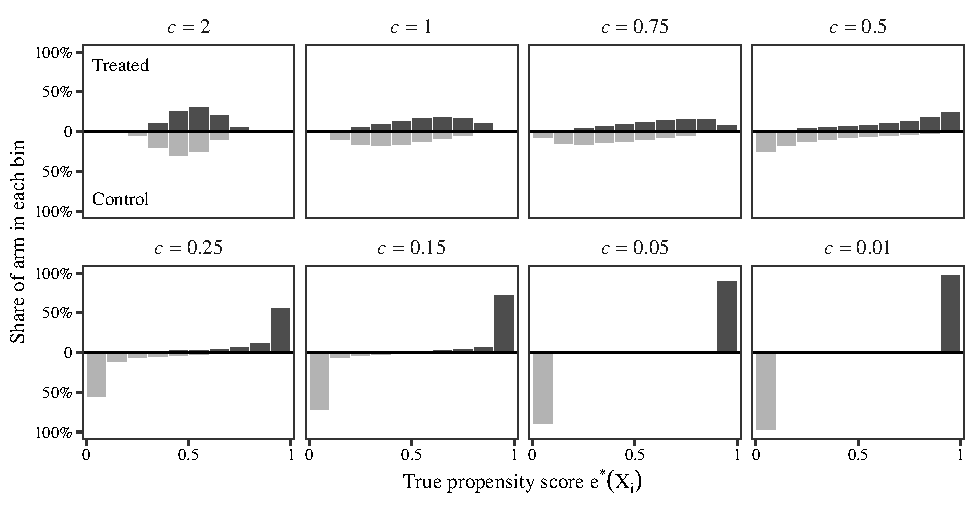
\includegraphics[keepaspectratio]{AAAAA-Working-Thesis_files/figure-pdf/unnamed-chunk-7-1.pdf}}

}

\caption{\label{afig-ov-levels}True propensity score by arm at each
overlap level \(c\), as the share of each arm in bins of width 0.1. The
outermost bins hold the units outside {[}0.1, 0.9{]}.}

\end{afig}%

\begin{atbl}

\caption{\label{atbl-ov-levels}Share of units with a true propensity
score \(e^*(X_i)\) outside each interval, by overlap level \(c\).}

\centering{

\begin{table}
\fontsize{8.0pt}{10.0pt}\selectfont
\begin{tabular*}{\linewidth}{@{\extracolsep{\fill}}rrrr}
\toprule
 & \multicolumn{3}{c}{{Outside}} \\ 
\cmidrule(lr){2-4}
\emph{c} & [0.1, 0.9] & [0.05, 0.95] & [0.01, 0.99] \\ 
\midrule\addlinespace[2.5pt]
2 & < 0.1\% & < 0.1\% & < 0.1\% \\ 
1 & 2.8\% & 0.3\% & < 0.1\% \\ 
0.75 & 9.9\% & 2.7\% & 0.1\% \\ 
0.5 & 27.2\% & 14.1\% & 2.2\% \\ 
0.25 & 58.3\% & 46.2\% & 25.1\% \\ 
0.15 & 74.2\% & 65.9\% & 49.1\% \\ 
0.05 & 91.3\% & 88.3\% & 81.8\% \\ 
0.01 & 98.2\% & 97.7\% & 96.3\% \\ 
\bottomrule
\end{tabular*}
\begin{minipage}{\linewidth}
\vspace{.05em}
\(c\) = 0.01 is used in the \(n\) × \(c\) grid only.\\
\end{minipage}
\end{table}

}

\end{atbl}%

\subsubsection*{Performance}\label{performance}
\addcontentsline{toc}{subsubsection}{Performance}

\begin{atbl}

\caption{\label{atbl-app-ov-full-c}Bias and RMSE under correct
specification, linear outcome, \(n\) = 1000 and 10 000.}

\centering{

\begingroup
\fontsize{8.0pt}{10.0pt}\selectfont
\setlength{\LTpost}{0mm}
\begin{longtable*}{llrrrrrr}
\toprule
 &  & \multicolumn{3}{c}{{n = 1000}} & \multicolumn{3}{c}{{n = 10000}} \\ 
\cmidrule(lr){3-5} \cmidrule(lr){6-8}
 & Overlap \emph{c} & 0.15 & 0.25 & 0.5 & 0.15 & 0.25 & 0.5 \\ 
\midrule\endhead\addlinespace[2.5pt]
{balnet} & {Bias} & {−0.699} & {−0.377} & {−0.013} & {−0.303} & {−0.002} & {−0.001} \\ 
{} & {RMSE} & {0.725} & {0.414} & {0.126} & {0.339} & {0.095} & {0.036} \\ 
{glmnet (Hájek)} & {Bias} & {−1.326} & {−0.877} & {−0.452} & {−0.766} & {−0.380} & {−0.155} \\ 
{} & {RMSE} & {1.348} & {0.922} & {0.476} & {0.856} & {0.480} & {0.177} \\ 
\bottomrule
\end{longtable*}
\begin{minipage}{\linewidth}
\vspace{.05em}
Largest MCSE: 0.0038 (Bias), 0.0033 (RMSE). No estimate is missing. τ = 0. balnet paths ending above λ = 1.01e-4: in 5 of 6 cells, up to 10 000 (treated) and 10 000 (control) per cell.\\
\end{minipage}
\endgroup

}

\end{atbl}%

\begin{atbl}

\caption{\label{atbl-app-ov-full-m}RMSE under a misspecified propensity
score, \(n\) = 1000 and 10 000.}

\centering{

\begingroup
\fontsize{8.0pt}{10.0pt}\selectfont
\setlength{\LTpost}{0mm}
\begin{longtable*}{llrrrr}
\toprule
 &  & \multicolumn{2}{c}{{n = 1000}} & \multicolumn{2}{c}{{n = 10000}} \\ 
\cmidrule(lr){3-4} \cmidrule(lr){5-6}
 & Overlap \emph{c} & 0.05 & 0.15 & 0.05 & 0.15 \\ 
\midrule\endhead\addlinespace[2.5pt]
\multicolumn{6}{l}{Linear} \\[2.5pt] 
\midrule\addlinespace[2.5pt]
{balnet} & {RMSE} & {1.376} & {1.022} & {1.316} & {0.753} \\ 
{ABW-balnet} & {RMSE} & {1.089} & {0.809} & {1.154} & {0.706} \\ 
{glmnet (Hájek)} & {RMSE} & {1.676} & {1.382} & {1.565} & {1.108} \\ 
{AIPW-glmnet} & {RMSE} & {1.159} & {1.039} & {1.970} & {1.751} \\ 
\midrule\addlinespace[2.5pt]
\multicolumn{6}{l}{Quadratic} \\[2.5pt] 
\midrule\addlinespace[2.5pt]
{balnet} & {RMSE} & {1.458} & {1.038} & {1.285} & {0.471} \\ 
{ABW-balnet} & {RMSE} & {1.163} & {0.831} & {1.084} & {0.425} \\ 
{glmnet (Hájek)} & {RMSE} & {1.724} & {1.453} & {1.413} & {1.207} \\ 
{AIPW-glmnet} & {RMSE} & {0.997} & {0.931} & {1.148} & {1.225} \\ 
\midrule\addlinespace[2.5pt]
\multicolumn{6}{l}{Exponential} \\[2.5pt] 
\midrule\addlinespace[2.5pt]
{balnet} & {RMSE} & {1.193} & {0.873} & {1.102} & {0.558} \\ 
{ABW-balnet} & {RMSE} & {1.049} & {0.766} & {0.999} & {0.528} \\ 
{glmnet (Hájek)} & {RMSE} & {1.384} & {1.160} & {1.365} & {1.005} \\ 
{AIPW-glmnet} & {RMSE} & {1.002} & {0.863} & {1.093} & {0.910} \\ 
\bottomrule
\end{longtable*}
\begin{minipage}{\linewidth}
\vspace{.05em}
Largest MCSE: 0.022 (RMSE). No estimate is missing. τ = 0.\\
\end{minipage}
\endgroup

}

\end{atbl}%

\subsubsection*{Coverage}\label{coverage}
\addcontentsline{toc}{subsubsection}{Coverage}

\begin{afig}

\centering{

\pandocbounded{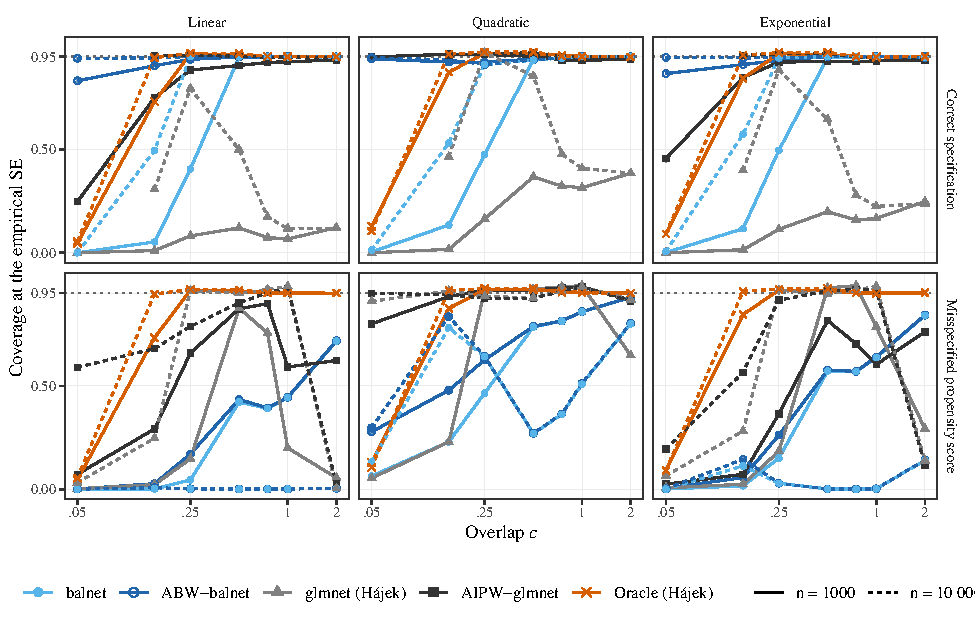
\includegraphics[keepaspectratio]{AAAAA-Working-Thesis_files/figure-pdf/unnamed-chunk-11-1.pdf}}

}

\caption{\label{afig-ov-coverage}Coverage at the empirical SE by overlap
\(c\) at \(n\) = 1000 and 10 000, both specifications. The dotted line
is the nominal 95\%.}

\end{afig}%

\subsection*{Appendix D: Overlap and sample size}\label{sec-app-nc}
\addcontentsline{toc}{subsection}{Appendix D: Overlap and sample size}

\subsubsection*{Performance}\label{performance-1}
\addcontentsline{toc}{subsubsection}{Performance}

\begin{afig}

\centering{

\pandocbounded{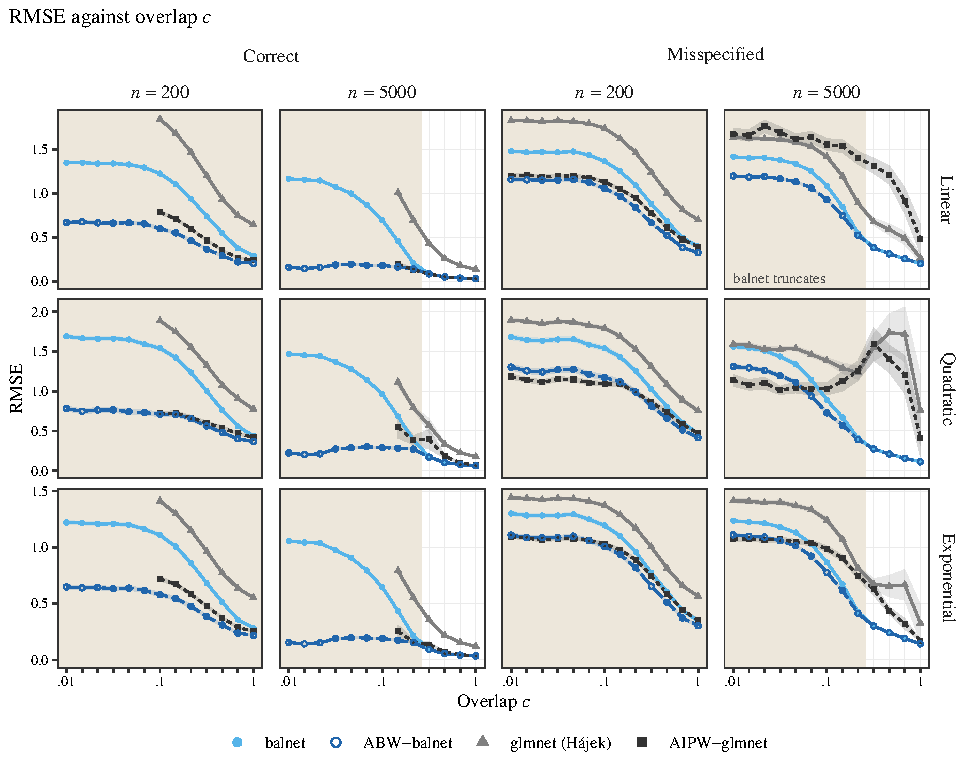
\includegraphics[keepaspectratio]{AAAAA-Working-Thesis_files/figure-pdf/unnamed-chunk-12-1.pdf}}

}

\caption{\label{afig-app-nc}RMSE against overlap \(c\) = 0.01 to 1 at
\(n\) = 200 and 5000, both specifications. Shading marks where the
balnet path truncates in at least half the replications
(Appendix Table~\ref{atbl-app-nc-trunc}). Modelling estimators are not
drawn where more than 1\% of replications have undefined weights.}

\end{afig}%

\begin{atbl}

\caption{\label{atbl-app-nc-full-m}RMSE under a misspecified propensity
score at the two weakest overlaps.}

\centering{

\begingroup
\fontsize{8.0pt}{10.0pt}\selectfont
\setlength{\LTpost}{0mm}
\begin{longtable*}{llrr}
\toprule
 &  & \multicolumn{2}{c}{{Overlap \emph{c}}} \\ 
\cmidrule(lr){3-4}
 &  & 0.01 & 0.0147 \\ 
\midrule\endhead\addlinespace[2.5pt]
\multicolumn{4}{l}{Linear · n = 200} \\[2.5pt] 
\midrule\addlinespace[2.5pt]
{balnet} & {RMSE} & {1.480} & {1.471} \\ 
{ABW-balnet} & {RMSE} & {1.161} & {1.156} \\ 
{glmnet (Hájek)} & {RMSE} & {1.829} & {1.828} \\ 
{AIPW-glmnet} & {RMSE} & {1.202} & {1.208} \\ 
\midrule\addlinespace[2.5pt]
\multicolumn{4}{l}{Linear · n = 5000} \\[2.5pt] 
\midrule\addlinespace[2.5pt]
{balnet} & {RMSE} & {1.418} & {1.405} \\ 
{ABW-balnet} & {RMSE} & {1.200} & {1.187} \\ 
{glmnet (Hájek)} & {RMSE} & {1.639} & {1.630} \\ 
{AIPW-glmnet} & {RMSE} & {1.681} & {1.661} \\ 
\midrule\addlinespace[2.5pt]
\multicolumn{4}{l}{Quadratic · n = 200} \\[2.5pt] 
\midrule\addlinespace[2.5pt]
{balnet} & {RMSE} & {1.680} & {1.644} \\ 
{ABW-balnet} & {RMSE} & {1.302} & {1.256} \\ 
{glmnet (Hájek)} & {RMSE} & {1.893} & {1.878} \\ 
{AIPW-glmnet} & {RMSE} & {1.183} & {1.141} \\ 
\midrule\addlinespace[2.5pt]
\multicolumn{4}{l}{Quadratic · n = 5000} \\[2.5pt] 
\midrule\addlinespace[2.5pt]
{balnet} & {RMSE} & {1.562} & {1.542} \\ 
{ABW-balnet} & {RMSE} & {1.310} & {1.293} \\ 
{glmnet (Hájek)} & {RMSE} & {1.593} & {1.577} \\ 
{AIPW-glmnet} & {RMSE} & {1.137} & {1.078} \\ 
\midrule\addlinespace[2.5pt]
\multicolumn{4}{l}{Exponential · n = 200} \\[2.5pt] 
\midrule\addlinespace[2.5pt]
{balnet} & {RMSE} & {1.301} & {1.284} \\ 
{ABW-balnet} & {RMSE} & {1.109} & {1.088} \\ 
{glmnet (Hájek)} & {RMSE} & {1.440} & {1.436} \\ 
{AIPW-glmnet} & {RMSE} & {1.094} & {1.082} \\ 
\midrule\addlinespace[2.5pt]
\multicolumn{4}{l}{Exponential · n = 5000} \\[2.5pt] 
\midrule\addlinespace[2.5pt]
{balnet} & {RMSE} & {1.237} & {1.223} \\ 
{ABW-balnet} & {RMSE} & {1.111} & {1.098} \\ 
{glmnet (Hájek)} & {RMSE} & {1.414} & {1.410} \\ 
{AIPW-glmnet} & {RMSE} & {1.075} & {1.075} \\ 
\bottomrule
\end{longtable*}
\begin{minipage}{\linewidth}
\vspace{.05em}
Largest MCSE: 0.037 (RMSE). No estimate is missing. τ = 0.\\
\end{minipage}
\endgroup

}

\end{atbl}%

\subsubsection*{Path truncation}\label{path-truncation}
\addcontentsline{toc}{subsubsection}{Path truncation}

\begin{atbl}

\caption{\label{atbl-app-nc-trunc}Replications (\%) in which the balnet
path truncates in at least one arm.}

\centering{

\begingroup
\fontsize{8.0pt}{10.0pt}\selectfont
\setlength{\LTpost}{0mm}
\begin{longtable*}{l|rrrrrrrrrrrrr}
\toprule
 & \multicolumn{13}{c}{{Overlap \emph{c}}} \\ 
\cmidrule(lr){2-14}
\emph{n} & 0.01 & 0.0147 & 0.0215 & 0.0316 & 0.0464 & 0.0681 & 0.1 & 0.147 & 0.215 & 0.316 & 0.464 & 0.681 & 1 \\ 
\midrule\endhead\addlinespace[2.5pt]
\multicolumn{14}{l}{Correct specification} \\[2.5pt] 
\midrule\addlinespace[2.5pt]
\multicolumn{1}{l}{{140}} & 100 & 100 & 100 & 100 & 100 & 100 & 100 & 100 & 100 & 100 & 100 & 100 & 100 \\ 
\multicolumn{1}{l}{{200}} & 100 & 100 & 100 & 100 & 100 & 100 & 100 & 100 & 100 & 100 & 100 & 100 & 100 \\ 
\multicolumn{1}{l}{{290}} & 100 & 100 & 100 & 100 & 100 & 100 & 100 & 100 & 100 & 100 & 100 & 100 & 99 \\ 
\multicolumn{1}{l}{{3500}} & 100 & 100 & 100 & 100 & 100 & 100 & 100 & 100 & 100 & 31 & 0 & 0 & 0 \\ 
\multicolumn{1}{l}{{5000}} & 100 & 100 & 100 & 100 & 100 & 100 & 100 & 100 & 100 & 0 & 0 & 0 & 0 \\ 
\midrule\addlinespace[2.5pt]
\multicolumn{14}{l}{Misspecified propensity score} \\[2.5pt] 
\midrule\addlinespace[2.5pt]
\multicolumn{1}{l}{{140}} & 100 & 100 & 100 & 100 & 100 & 100 & 100 & 100 & 100 & 100 & 100 & 100 & 100 \\ 
\multicolumn{1}{l}{{200}} & 100 & 100 & 100 & 100 & 100 & 100 & 100 & 100 & 100 & 100 & 100 & 100 & 100 \\ 
\multicolumn{1}{l}{{290}} & 100 & 100 & 100 & 100 & 100 & 100 & 100 & 100 & 100 & 100 & 100 & 100 & 98 \\ 
\multicolumn{1}{l}{{3500}} & 100 & 100 & 100 & 100 & 100 & 100 & 100 & 100 & 100 & 4 & 0 & 0 & 0 \\ 
\multicolumn{1}{l}{{5000}} & 100 & 100 & 100 & 100 & 100 & 100 & 100 & 100 & 96 & 0 & 0 & 0 & 0 \\ 
\bottomrule
\end{longtable*}
\begin{minipage}{\linewidth}
\vspace{.05em}
Truncated: the path ends above λ = 1.01e-4. Largest MCSE: 1.5 percentage points.\\
\end{minipage}
\endgroup

}

\end{atbl}%

\subsection*{Appendix E: High-dimensional settings}\label{sec-app-pn}
\addcontentsline{toc}{subsection}{Appendix E: High-dimensional settings}

\subsubsection*{Performance}\label{performance-2}
\addcontentsline{toc}{subsubsection}{Performance}

\begin{afig}

\centering{

\pandocbounded{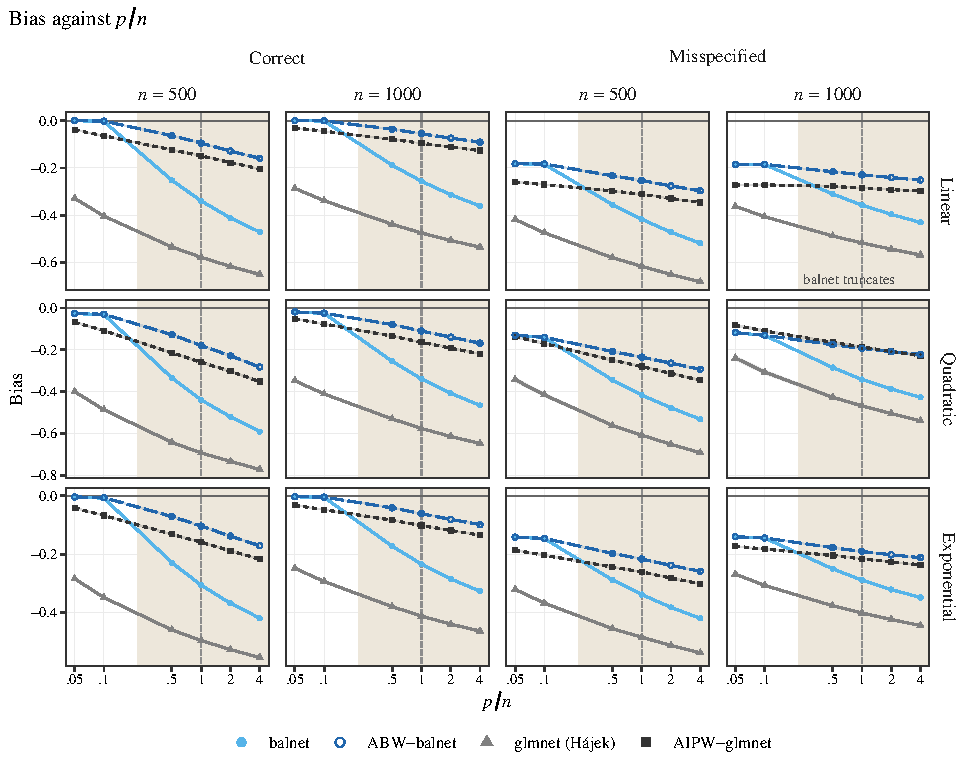
\includegraphics[keepaspectratio]{AAAAA-Working-Thesis_files/figure-pdf/unnamed-chunk-15-1.pdf}}

}

\caption{\label{afig-app-pn-bias}Bias against \(p/n\) at \(n\) = 500 and
1000, both specifications. Shading and dotted line as in
Figure~\ref{fig-pn-rmse}.}

\end{afig}%

\begin{atbl}

\caption{\label{atbl-app-pn-full-c}Bias and RMSE under correct
specification, by outcome.}

\centering{

\begingroup
\fontsize{8.0pt}{10.0pt}\selectfont
\setlength{\LTpost}{0mm}
\begin{longtable*}{llrrrrr}
\toprule
 &  & \multicolumn{5}{c}{{\emph{p}/\emph{n}}} \\ 
\cmidrule(lr){3-7}
 &  & 0.1 & 0.5 & 1 & 2 & 4 \\ 
\midrule\endhead\addlinespace[2.5pt]
\multicolumn{7}{l}{Linear · n = 500} \\[2.5pt] 
\midrule\addlinespace[2.5pt]
{balnet} & {Bias} & {−0.003} & {−0.252} & {−0.340} & {−0.412} & {−0.471} \\ 
{} & {RMSE} & {0.121} & {0.276} & {0.357} & {0.426} & {0.483} \\ 
{ABW-balnet} & {Bias} & {−0.002} & {−0.063} & {−0.095} & {−0.129} & {−0.159} \\ 
{} & {RMSE} & {0.121} & {0.129} & {0.143} & {0.166} & {0.190} \\ 
{glmnet (Hájek)} & {Bias} & {−0.404} & {−0.535} & {−0.579} & {−0.617} & {−0.651} \\ 
{} & {RMSE} & {0.420} & {0.546} & {0.589} & {0.627} & {0.660} \\ 
{AIPW-glmnet} & {Bias} & {−0.064} & {−0.123} & {−0.149} & {−0.177} & {−0.204} \\ 
{} & {RMSE} & {0.120} & {0.160} & {0.180} & {0.205} & {0.228} \\ 
{Oracle (Hájek)} & {Bias} & {−0.012} & {−0.008} & {−0.006} & {−0.005} & {−0.008} \\ 
{} & {RMSE} & {0.198} & {0.196} & {0.199} & {0.199} & {0.200} \\ 
\midrule\addlinespace[2.5pt]
\multicolumn{7}{l}{Linear · n = 1000} \\[2.5pt] 
\midrule\addlinespace[2.5pt]
{balnet} & {Bias} & {−0.001} & {−0.188} & {−0.256} & {−0.314} & {−0.361} \\ 
{} & {RMSE} & {0.083} & {0.204} & {0.267} & {0.322} & {0.369} \\ 
{ABW-balnet} & {Bias} & {0.000} & {−0.036} & {−0.055} & {−0.074} & {−0.091} \\ 
{} & {RMSE} & {0.083} & {0.086} & {0.094} & {0.105} & {0.117} \\ 
{glmnet (Hájek)} & {Bias} & {−0.339} & {−0.439} & {−0.475} & {−0.507} & {−0.536} \\ 
{} & {RMSE} & {0.348} & {0.445} & {0.481} & {0.513} & {0.541} \\ 
{AIPW-glmnet} & {Bias} & {−0.045} & {−0.079} & {−0.096} & {−0.111} & {−0.126} \\ 
{} & {RMSE} & {0.084} & {0.106} & {0.119} & {0.132} & {0.145} \\ 
{Oracle (Hájek)} & {Bias} & {−0.004} & {−0.004} & {−0.005} & {−0.005} & {−0.003} \\ 
{} & {RMSE} & {0.142} & {0.139} & {0.141} & {0.142} & {0.142} \\ 
\midrule\addlinespace[2.5pt]
\multicolumn{7}{l}{Quadratic · n = 500} \\[2.5pt] 
\midrule\addlinespace[2.5pt]
{balnet} & {Bias} & {−0.032} & {−0.335} & {−0.440} & {−0.521} & {−0.592} \\ 
{} & {RMSE} & {0.221} & {0.390} & {0.480} & {0.555} & {0.621} \\ 
{ABW-balnet} & {Bias} & {−0.030} & {−0.128} & {−0.180} & {−0.229} & {−0.283} \\ 
{} & {RMSE} & {0.221} & {0.239} & {0.265} & {0.300} & {0.340} \\ 
{glmnet (Hájek)} & {Bias} & {−0.487} & {−0.643} & {−0.694} & {−0.734} & {−0.773} \\ 
{} & {RMSE} & {0.527} & {0.671} & {0.719} & {0.758} & {0.796} \\ 
{AIPW-glmnet} & {Bias} & {−0.109} & {−0.215} & {−0.260} & {−0.304} & {−0.352} \\ 
{} & {RMSE} & {0.230} & {0.289} & {0.323} & {0.360} & {0.401} \\ 
{Oracle (Hájek)} & {Bias} & {−0.012} & {−0.011} & {−0.007} & {−0.001} & {−0.008} \\ 
{} & {RMSE} & {0.299} & {0.296} & {0.300} & {0.306} & {0.301} \\ 
\midrule\addlinespace[2.5pt]
\multicolumn{7}{l}{Quadratic · n = 1000} \\[2.5pt] 
\midrule\addlinespace[2.5pt]
{balnet} & {Bias} & {−0.026} & {−0.255} & {−0.339} & {−0.408} & {−0.466} \\ 
{} & {RMSE} & {0.154} & {0.291} & {0.365} & {0.429} & {0.484} \\ 
{ABW-balnet} & {Bias} & {−0.025} & {−0.079} & {−0.110} & {−0.140} & {−0.168} \\ 
{} & {RMSE} & {0.153} & {0.163} & {0.175} & {0.195} & {0.215} \\ 
{glmnet (Hájek)} & {Bias} & {−0.412} & {−0.531} & {−0.577} & {−0.615} & {−0.649} \\ 
{} & {RMSE} & {0.435} & {0.548} & {0.592} & {0.629} & {0.662} \\ 
{AIPW-glmnet} & {Bias} & {−0.077} & {−0.135} & {−0.165} & {−0.192} & {−0.220} \\ 
{} & {RMSE} & {0.162} & {0.193} & {0.214} & {0.237} & {0.259} \\ 
{Oracle (Hájek)} & {Bias} & {−0.005} & {−0.003} & {−0.006} & {−0.006} & {−0.004} \\ 
{} & {RMSE} & {0.213} & {0.212} & {0.213} & {0.216} & {0.214} \\ 
\midrule\addlinespace[2.5pt]
\multicolumn{7}{l}{Exponential · n = 500} \\[2.5pt] 
\midrule\addlinespace[2.5pt]
{balnet} & {Bias} & {−0.008} & {−0.229} & {−0.306} & {−0.369} & {−0.419} \\ 
{} & {RMSE} & {0.130} & {0.259} & {0.327} & {0.386} & {0.435} \\ 
{ABW-balnet} & {Bias} & {−0.006} & {−0.071} & {−0.104} & {−0.138} & {−0.171} \\ 
{} & {RMSE} & {0.130} & {0.140} & {0.155} & {0.179} & {0.205} \\ 
{glmnet (Hájek)} & {Bias} & {−0.349} & {−0.460} & {−0.496} & {−0.527} & {−0.555} \\ 
{} & {RMSE} & {0.368} & {0.474} & {0.509} & {0.539} & {0.567} \\ 
{AIPW-glmnet} & {Bias} & {−0.068} & {−0.132} & {−0.159} & {−0.188} & {−0.217} \\ 
{} & {RMSE} & {0.131} & {0.172} & {0.194} & {0.219} & {0.244} \\ 
{Oracle (Hájek)} & {Bias} & {−0.009} & {−0.006} & {−0.004} & {−0.003} & {−0.005} \\ 
{} & {RMSE} & {0.182} & {0.181} & {0.183} & {0.184} & {0.184} \\ 
\midrule\addlinespace[2.5pt]
\multicolumn{7}{l}{Exponential · n = 1000} \\[2.5pt] 
\midrule\addlinespace[2.5pt]
{balnet} & {Bias} & {−0.005} & {−0.173} & {−0.234} & {−0.285} & {−0.327} \\ 
{} & {RMSE} & {0.090} & {0.192} & {0.247} & {0.295} & {0.336} \\ 
{ABW-balnet} & {Bias} & {−0.004} & {−0.041} & {−0.061} & {−0.081} & {−0.098} \\ 
{} & {RMSE} & {0.090} & {0.094} & {0.102} & {0.114} & {0.126} \\ 
{glmnet (Hájek)} & {Bias} & {−0.294} & {−0.380} & {−0.412} & {−0.440} & {−0.464} \\ 
{} & {RMSE} & {0.305} & {0.388} & {0.420} & {0.447} & {0.471} \\ 
{AIPW-glmnet} & {Bias} & {−0.048} & {−0.084} & {−0.102} & {−0.119} & {−0.135} \\ 
{} & {RMSE} & {0.092} & {0.114} & {0.128} & {0.142} & {0.156} \\ 
{Oracle (Hájek)} & {Bias} & {−0.003} & {−0.002} & {−0.004} & {−0.004} & {−0.002} \\ 
{} & {RMSE} & {0.131} & {0.129} & {0.130} & {0.131} & {0.131} \\ 
\bottomrule
\end{longtable*}
\begin{minipage}{\linewidth}
\vspace{.05em}
Largest MCSE: 0.0031 (Bias), 0.004 (RMSE). No estimate is missing. τ = 0.\\
\end{minipage}
\endgroup

}

\end{atbl}%

\begin{atbl}

\caption{\label{atbl-app-pn-full-m}Bias and RMSE under a misspecified
propensity score, by outcome.}

\centering{

\begingroup
\fontsize{8.0pt}{10.0pt}\selectfont
\setlength{\LTpost}{0mm}
\begin{longtable*}{llrrrrr}
\toprule
 &  & \multicolumn{5}{c}{{\emph{p}/\emph{n}}} \\ 
\cmidrule(lr){3-7}
 &  & 0.1 & 0.5 & 1 & 2 & 4 \\ 
\midrule\endhead\addlinespace[2.5pt]
\multicolumn{7}{l}{Linear · n = 500} \\[2.5pt] 
\midrule\addlinespace[2.5pt]
{balnet} & {Bias} & {−0.184} & {−0.355} & {−0.417} & {−0.472} & {−0.519} \\ 
{} & {RMSE} & {0.229} & {0.377} & {0.435} & {0.487} & {0.531} \\ 
{ABW-balnet} & {Bias} & {−0.183} & {−0.233} & {−0.253} & {−0.276} & {−0.297} \\ 
{} & {RMSE} & {0.229} & {0.267} & {0.283} & {0.302} & {0.320} \\ 
{glmnet (Hájek)} & {Bias} & {−0.475} & {−0.580} & {−0.616} & {−0.651} & {−0.683} \\ 
{} & {RMSE} & {0.500} & {0.594} & {0.628} & {0.662} & {0.692} \\ 
{AIPW-glmnet} & {Bias} & {−0.270} & {−0.297} & {−0.312} & {−0.330} & {−0.346} \\ 
{} & {RMSE} & {0.306} & {0.323} & {0.335} & {0.350} & {0.366} \\ 
\midrule\addlinespace[2.5pt]
\multicolumn{7}{l}{Linear · n = 1000} \\[2.5pt] 
\midrule\addlinespace[2.5pt]
{balnet} & {Bias} & {−0.186} & {−0.310} & {−0.357} & {−0.397} & {−0.431} \\ 
{} & {RMSE} & {0.209} & {0.323} & {0.368} & {0.405} & {0.438} \\ 
{ABW-balnet} & {Bias} & {−0.185} & {−0.216} & {−0.229} & {−0.241} & {−0.251} \\ 
{} & {RMSE} & {0.208} & {0.235} & {0.246} & {0.256} & {0.266} \\ 
{glmnet (Hájek)} & {Bias} & {−0.407} & {−0.488} & {−0.518} & {−0.544} & {−0.569} \\ 
{} & {RMSE} & {0.435} & {0.500} & {0.530} & {0.554} & {0.576} \\ 
{AIPW-glmnet} & {Bias} & {−0.272} & {−0.278} & {−0.285} & {−0.292} & {−0.298} \\ 
{} & {RMSE} & {0.312} & {0.299} & {0.305} & {0.309} & {0.312} \\ 
\midrule\addlinespace[2.5pt]
\multicolumn{7}{l}{Quadratic · n = 500} \\[2.5pt] 
\midrule\addlinespace[2.5pt]
{balnet} & {Bias} & {−0.141} & {−0.344} & {−0.417} & {−0.478} & {−0.532} \\ 
{} & {RMSE} & {0.260} & {0.401} & {0.461} & {0.515} & {0.565} \\ 
{ABW-balnet} & {Bias} & {−0.141} & {−0.208} & {−0.236} & {−0.264} & {−0.294} \\ 
{} & {RMSE} & {0.259} & {0.296} & {0.313} & {0.332} & {0.354} \\ 
{glmnet (Hájek)} & {Bias} & {−0.416} & {−0.562} & {−0.609} & {−0.652} & {−0.693} \\ 
{} & {RMSE} & {0.587} & {0.627} & {0.657} & {0.692} & {0.725} \\ 
{AIPW-glmnet} & {Bias} & {−0.170} & {−0.250} & {−0.280} & {−0.313} & {−0.346} \\ 
{} & {RMSE} & {0.314} & {0.340} & {0.358} & {0.379} & {0.405} \\ 
\midrule\addlinespace[2.5pt]
\multicolumn{7}{l}{Quadratic · n = 1000} \\[2.5pt] 
\midrule\addlinespace[2.5pt]
{balnet} & {Bias} & {−0.131} & {−0.285} & {−0.342} & {−0.388} & {−0.427} \\ 
{} & {RMSE} & {0.202} & {0.321} & {0.369} & {0.412} & {0.448} \\ 
{ABW-balnet} & {Bias} & {−0.131} & {−0.176} & {−0.194} & {−0.209} & {−0.223} \\ 
{} & {RMSE} & {0.201} & {0.231} & {0.241} & {0.253} & {0.263} \\ 
{glmnet (Hájek)} & {Bias} & {−0.307} & {−0.427} & {−0.468} & {−0.505} & {−0.541} \\ 
{} & {RMSE} & {0.595} & {0.523} & {0.566} & {0.580} & {0.583} \\ 
{AIPW-glmnet} & {Bias} & {−0.110} & {−0.164} & {−0.187} & {−0.208} & {−0.229} \\ 
{} & {RMSE} & {0.303} & {0.270} & {0.284} & {0.291} & {0.290} \\ 
\midrule\addlinespace[2.5pt]
\multicolumn{7}{l}{Exponential · n = 500} \\[2.5pt] 
\midrule\addlinespace[2.5pt]
{balnet} & {Bias} & {−0.147} & {−0.288} & {−0.338} & {−0.382} & {−0.420} \\ 
{} & {RMSE} & {0.201} & {0.316} & {0.361} & {0.401} & {0.436} \\ 
{ABW-balnet} & {Bias} & {−0.146} & {−0.197} & {−0.217} & {−0.239} & {−0.259} \\ 
{} & {RMSE} & {0.201} & {0.238} & {0.252} & {0.269} & {0.286} \\ 
{glmnet (Hájek)} & {Bias} & {−0.368} & {−0.455} & {−0.485} & {−0.513} & {−0.539} \\ 
{} & {RMSE} & {0.415} & {0.477} & {0.502} & {0.529} & {0.552} \\ 
{AIPW-glmnet} & {Bias} & {−0.203} & {−0.244} & {−0.261} & {−0.282} & {−0.301} \\ 
{} & {RMSE} & {0.240} & {0.274} & {0.288} & {0.307} & {0.325} \\ 
\midrule\addlinespace[2.5pt]
\multicolumn{7}{l}{Exponential · n = 1000} \\[2.5pt] 
\midrule\addlinespace[2.5pt]
{balnet} & {Bias} & {−0.145} & {−0.250} & {−0.289} & {−0.321} & {−0.348} \\ 
{} & {RMSE} & {0.174} & {0.266} & {0.302} & {0.332} & {0.358} \\ 
{ABW-balnet} & {Bias} & {−0.144} & {−0.178} & {−0.191} & {−0.202} & {−0.212} \\ 
{} & {RMSE} & {0.174} & {0.201} & {0.211} & {0.220} & {0.229} \\ 
{glmnet (Hájek)} & {Bias} & {−0.307} & {−0.377} & {−0.402} & {−0.424} & {−0.445} \\ 
{} & {RMSE} & {0.377} & {0.401} & {0.428} & {0.444} & {0.458} \\ 
{AIPW-glmnet} & {Bias} & {−0.183} & {−0.205} & {−0.216} & {−0.226} & {−0.236} \\ 
{} & {RMSE} & {0.210} & {0.225} & {0.236} & {0.244} & {0.253} \\ 
\bottomrule
\end{longtable*}
\begin{minipage}{\linewidth}
\vspace{.05em}
Largest MCSE: 0.0051 (Bias), 0.051 (RMSE). No estimate is missing. τ = 0.\\
\end{minipage}
\endgroup

}

\end{atbl}%

\subsubsection*{Fit diagnostics}\label{fit-diagnostics-1}
\addcontentsline{toc}{subsubsection}{Fit diagnostics}

\begin{atbl}

\caption{\label{atbl-app-pn-diag-c-lin}Nonzero coefficients of balnet
and the glmnet propensity score under correct specification, linear
outcome. Median (lower--upper quartile) across replications.}

\centering{

\begingroup
\fontsize{8.0pt}{10.0pt}\selectfont
\setlength{\LTpost}{0mm}
\begin{longtable*}{llrrrrr}
\toprule
 &  & \multicolumn{5}{c}{{\emph{p}/\emph{n}}} \\ 
\cmidrule(lr){3-7}
 &  & 0.1 & 0.5 & 1 & 2 & 4 \\ 
\midrule\endhead\addlinespace[2.5pt]
\multicolumn{7}{l}{Nonzero coefficients · n = 500} \\[2.5pt] 
\midrule\addlinespace[2.5pt]
{glmnet PS} & {Both} & {10 (7–14)} & {12 (7–19)} & {12 (7–21)} & {12 (6–23)} & {12 (6–23)} \\ 
{balnet} & {Treated} & {50 (50–50)} & {102 (94–109)} & {109 (99–120)} & {111 (98–127)} & {109 (92–129)} \\ 
{} & {Control} & {50 (50–50)} & {101 (94–109)} & {109 (99–119)} & {110 (97–126)} & {109 (92–129)} \\ 
\midrule\addlinespace[2.5pt]
\multicolumn{7}{l}{Nonzero coefficients · n = 1000} \\[2.5pt] 
\midrule\addlinespace[2.5pt]
{glmnet PS} & {Both} & {13 (9–19)} & {16 (10–25)} & {16 (10–26)} & {17 (10–28)} & {17 (9–29)} \\ 
{balnet} & {Treated} & {100 (100–100)} & {197 (185–209)} & {210 (192–230)} & {211 (187–242)} & {208 (177–246)} \\ 
{} & {Control} & {100 (100–100)} & {197 (185–209)} & {210 (191–230)} & {211 (187–242)} & {207 (177–246)} \\ 
\bottomrule
\end{longtable*}
\begin{minipage}{\linewidth}
\vspace{.05em}
No MCSE, as these describe the fits. Nonzero coefficients at lambda.min: the glmnet propensity score, one fit for both arms. balnet paths ending above λ = 1.01e-4: in 10 of 10 cells, up to 10 000 (treated) and 10 000 (control) per cell.\\
\end{minipage}
\endgroup

}

\end{atbl}%

\begin{atbl}

\caption{\label{atbl-app-pn-diag-m-lin}Nonzero coefficients of balnet
and the glmnet propensity score under a misspecified propensity score,
linear outcome. Median (lower--upper quartile) across replications.}

\centering{

\begingroup
\fontsize{8.0pt}{10.0pt}\selectfont
\setlength{\LTpost}{0mm}
\begin{longtable*}{llrrrrr}
\toprule
 &  & \multicolumn{5}{c}{{\emph{p}/\emph{n}}} \\ 
\cmidrule(lr){3-7}
 &  & 0.1 & 0.5 & 1 & 2 & 4 \\ 
\midrule\endhead\addlinespace[2.5pt]
\multicolumn{7}{l}{Nonzero coefficients · n = 500} \\[2.5pt] 
\midrule\addlinespace[2.5pt]
{glmnet PS} & {Both} & {8 (5–11)} & {9 (5–15)} & {10 (6–17)} & {11 (6–19)} & {11 (6–21)} \\ 
{balnet} & {Treated} & {50 (50–50)} & {102 (95–110)} & {110 (99–121)} & {112 (98–128)} & {110 (93–131)} \\ 
{} & {Control} & {50 (50–50)} & {106 (99–113)} & {113 (103–124)} & {114 (101–131)} & {111 (95–133)} \\ 
\midrule\addlinespace[2.5pt]
\multicolumn{7}{l}{Nonzero coefficients · n = 1000} \\[2.5pt] 
\midrule\addlinespace[2.5pt]
{glmnet PS} & {Both} & {9 (6–14)} & {11 (7–18)} & {11 (6–19)} & {12 (7–21)} & {12 (7–22)} \\ 
{balnet} & {Treated} & {100 (100–100)} & {201 (188–213)} & {213 (195–234)} & {216 (191–246)} & {212 (181–251)} \\ 
{} & {Control} & {100 (100–100)} & {207 (195–219)} & {219 (201–241)} & {220 (195–250)} & {216 (184–256)} \\ 
\bottomrule
\end{longtable*}
\begin{minipage}{\linewidth}
\vspace{.05em}
No MCSE, as these describe the fits. Nonzero coefficients at lambda.min: the glmnet propensity score, one fit for both arms. balnet paths ending above λ = 1.01e-4: in 10 of 10 cells, up to 10 000 (treated) and 10 000 (control) per cell.\\
\end{minipage}
\endgroup

}

\end{atbl}%

\subsection*{Appendix F: Sparsity grid}\label{sec-app-sp}
\addcontentsline{toc}{subsection}{Appendix F: Sparsity grid}

\subsubsection*{Performance}\label{performance-3}
\addcontentsline{toc}{subsubsection}{Performance}

\begin{atbl}

\caption{\label{atbl-app-sp-cells}Bias, RMSE and nonzero coefficients of
the glmnet propensity score once the balnet path truncates, under
correct specification.}

\centering{

\begingroup
\fontsize{8.0pt}{10.0pt}\selectfont
\setlength{\LTpost}{0mm}
\begin{longtable*}{lllrrrrrrr}
\toprule
 &  &  & \multicolumn{4}{c}{{Bias}} & \multicolumn{2}{c}{{RMSE}} & \multicolumn{1}{c}{{Propensity score}} \\ 
\cmidrule(lr){4-7} \cmidrule(lr){8-9} \cmidrule(lr){10-10}
Covariates & \emph{ν} & \emph{s} & balnet & ABW & Hájek & AIPW & ABW & AIPW & Nonzero \\ 
\midrule\endhead\addlinespace[2.5pt]
independent & 1 & 4 & −0.171 & −0.074 & −0.329 & −0.122 & 0.129 & 0.159 & 10–16 \\ 
 &  & 16 & −0.207 & −0.117 & −0.376 & −0.186 & 0.158 & 0.212 & 13–21 \\ 
 &  & 64 & −0.223 & −0.137 & −0.393 & −0.209 & 0.174 & 0.233 & 13–22 \\ 
 & 0.5 & 4 & −0.183 & −0.075 & −0.354 & −0.132 & 0.130 & 0.166 & 12–20 \\ 
 &  & 16 & −0.296 & −0.197 & −0.490 & −0.300 & 0.225 & 0.318 & 22–41 \\ 
 &  & 64 & −0.374 & −0.308 & −0.579 & −0.447 & 0.328 & 0.460 & 21–52 \\ 
AR(1) & 1 & 4 & −0.122 & −0.039 & −0.278 & −0.071 & 0.108 & 0.120 & 7–11 \\ 
 &  & 16 & −0.146 & −0.058 & −0.327 & −0.116 & 0.118 & 0.151 & 12–19 \\ 
 &  & 64 & −0.157 & −0.072 & −0.346 & −0.140 & 0.125 & 0.171 & 15–22 \\ 
 & 0.5 & 4 & −0.126 & −0.038 & −0.285 & −0.073 & 0.110 & 0.122 & 8–12 \\ 
 &  & 16 & −0.176 & −0.076 & −0.376 & −0.148 & 0.128 & 0.176 & 17–29 \\ 
 &  & 64 & −0.230 & −0.140 & −0.466 & −0.256 & 0.174 & 0.274 & 30–50 \\ 
equicorrelated & 1 & 4 & −0.091 & −0.047 & −0.212 & −0.059 & 0.111 & 0.119 & 10–22 \\ 
 &  & 16 & −0.062 & −0.036 & −0.189 & −0.044 & 0.106 & 0.110 & 13–29 \\ 
 &  & 64 & −0.047 & −0.028 & −0.178 & −0.034 & 0.104 & 0.107 & 20–32 \\ 
 & 0.5 & 4 & −0.088 & −0.046 & −0.214 & −0.061 & 0.110 & 0.117 & 11–24 \\ 
 &  & 16 & −0.053 & −0.037 & −0.184 & −0.046 & 0.107 & 0.109 & 14–33 \\ 
 &  & 64 & −0.029 & −0.019 & −0.162 & −0.022 & 0.101 & 0.103 & 21–34 \\ 
\bottomrule
\end{longtable*}
\begin{minipage}{\linewidth}
\vspace{.05em}
Means over the 8 cells of each row (\(n\) = 500 and 1000, \(p/n\) = 0.5 and 1, linear and quadratic outcomes), at 1000 Monte Carlo replications per cell. Largest MCSE: 0.0035 (bias), 0.0034 (RMSE). Nonzero: range of the per-cell median nonzero coefficients of the glmnet propensity score, over \(p/n\) = 0.1 to 1. ABW has the lower RMSE in all 96 cells with independent or AR(1) covariates. While exact balance holds (\(p/n\) = 0.1) the absolute bias of balnet is at most 0.006 (linear) and 0.028 (quadratic).\\
\end{minipage}
\endgroup

}

\end{atbl}%

\subsubsection*{Imbalance bound}\label{imbalance-bound}
\addcontentsline{toc}{subsubsection}{Imbalance bound}

\begin{atbl}

\caption{\label{atbl-app-sp-bound}Linear-outcome bias of balnet as a
percentage of the imbalance bound, the sum of the two arms' mean path
ends times the \(\ell_1\) norm of the outcome coefficient.}

\centering{

\begingroup
\fontsize{8.0pt}{10.0pt}\selectfont
\setlength{\LTpost}{0mm}
\begin{longtable*}{rrcrrrr}
\toprule
 &  &  & \multicolumn{2}{c}{{\emph{n} = 500, \emph{p}/\emph{n}}} & \multicolumn{2}{c}{{\emph{n} = 1000, \emph{p}/\emph{n}}} \\ 
\cmidrule(lr){4-5} \cmidrule(lr){6-7}
\emph{s} & \emph{ν} & Covariates & 0.5 & 1 & 0.5 & 1 \\ 
\midrule\endhead\addlinespace[2.5pt]
4 & 1.0 & independent & 98 & 97 & 99 & 100 \\ 
4 & 1.0 & AR(1) & 94 & 99 & 100 & 98 \\ 
4 & 0.5 & independent & 99 & 99 & 100 & 100 \\ 
4 & 0.5 & AR(1) & 96 & 98 & 99 & 101 \\ 
16 & 1.0 & independent & 78 & 77 & 85 & 83 \\ 
16 & 1.0 & AR(1) & 79 & 83 & 86 & 86 \\ 
16 & 0.5 & independent & 88 & 87 & 95 & 95 \\ 
16 & 0.5 & AR(1) & 80 & 84 & 91 & 93 \\ 
64 & 1.0 & independent & 60 & 60 & 67 & 66 \\ 
64 & 1.0 & AR(1) & 62 & 63 & 69 & 70 \\ 
64 & 0.5 & independent & 60 & 58 & 72 & 71 \\ 
64 & 0.5 & AR(1) & 57 & 64 & 68 & 73 \\ 
\bottomrule
\end{longtable*}
\begin{minipage}{\linewidth}
\vspace{.05em}
Largest MCSE: 2.7 points; values above 100 are within 1 MCSE of 100. The \(\ell_1\) norm is \(\sum_{j \le s} j^{-\nu} / \sigma_g\).\\
\end{minipage}
\endgroup

}

\end{atbl}%

\subsubsection*{Averages}\label{averages-1}
\addcontentsline{toc}{subsubsection}{Averages}

\begin{atbl}

\caption{\label{atbl-app-sp-exact}Per cent lower RMSE \(\bar R(\Theta)\)
and share of bias \(\bar s_m(\Theta)\) of A against B at exact balance
(\(p/n\) = 0.1).}

\centering{

\begingroup
\fontsize{8.0pt}{10.0pt}\selectfont
\setlength{\LTpost}{0mm}
\begin{longtable*}{l|>{\raggedleft\arraybackslash}p{\dimexpr 70.00pt -2\tabcolsep-1.5\arrayrulewidth}>{\raggedleft\arraybackslash}p{\dimexpr 70.00pt -2\tabcolsep-1.5\arrayrulewidth}>{\raggedleft\arraybackslash}p{\dimexpr 70.00pt -2\tabcolsep-1.5\arrayrulewidth}rr}
\toprule
 & \multicolumn{3}{>{\centering\arraybackslash}m{\dimexpr 210.00pt -2\tabcolsep-1.5\arrayrulewidth}}{\parbox{\linewidth}{\centering {\(\bar R(\Theta)\), A vs B}}} & \multicolumn{2}{c}{{\(\bar s_m(\Theta)\)}} \\ 
\cmidrule(lr){2-4} \cmidrule(lr){5-6}
 & balnet vs glmnet (Hájek) & balnet vs AIPW-glmnet & ABW-balnet vs AIPW-glmnet & balnet & glmnet (Hájek) \\ 
\midrule\endhead\addlinespace[2.5pt]
\multicolumn{6}{l}{Overall} \\[2.5pt] 
\midrule\addlinespace[2.5pt]
all cells & 55.6 & 6.1 & 6.1 & 0.01 & 0.80 \\ 
\midrule\addlinespace[2.5pt]
\multicolumn{6}{l}{Confounders s} \\[2.5pt] 
\midrule\addlinespace[2.5pt]
4 & 55.8 & 0.5 & 0.5 & 0.02 & 0.81 \\ 
16 & 59.3 & 10.3 & 10.3 & 0.01 & 0.83 \\ 
64 & 60.9 & 15.6 & 15.6 & 0.01 & 0.82 \\ 
\midrule\addlinespace[2.5pt]
\multicolumn{6}{l}{Decay ν} \\[2.5pt] 
\midrule\addlinespace[2.5pt]
0.5 & 57.0 & 7.6 & 7.6 & 0.01 & 0.81 \\ 
1 & 54.1 & 4.6 & 4.6 & 0.02 & 0.79 \\ 
\midrule\addlinespace[2.5pt]
\multicolumn{6}{l}{Covariates} \\[2.5pt] 
\midrule\addlinespace[2.5pt]
independent & 63.6 & 18.1 & 18.1 & 0.01 & 0.88 \\ 
AR(1) & 58.2 & 2.7 & 2.7 & 0.01 & 0.84 \\ 
equicorrelated & 42.4 & -3.8 & -3.8 & 0.02 & 0.69 \\ 
\midrule\addlinespace[2.5pt]
\multicolumn{6}{l}{Independent covariates, confounders s} \\[2.5pt] 
\midrule\addlinespace[2.5pt]
4 & 62.2 & 5.8 & 5.8 & 0.01 & 0.87 \\ 
16 & 67.5 & 24.2 & 24.2 & 0.01 & 0.91 \\ 
64 & 71.1 & 35.0 & 35.0 & 0.01 & 0.92 \\ 
\midrule\addlinespace[2.5pt]
\multicolumn{6}{l}{AR(1) covariates, confounders s} \\[2.5pt] 
\midrule\addlinespace[2.5pt]
4 & 56.5 & -2.7 & -2.7 & 0.02 & 0.83 \\ 
16 & 62.6 & 5.4 & 5.4 & 0.01 & 0.88 \\ 
64 & 65.3 & 12.5 & 12.5 & 0.01 & 0.89 \\ 
\midrule\addlinespace[2.5pt]
\multicolumn{6}{l}{Equicorrelated covariates, confounders s} \\[2.5pt] 
\midrule\addlinespace[2.5pt]
4 & 47.7 & -1.7 & -1.7 & 0.03 & 0.74 \\ 
16 & 44.6 & -0.8 & -0.8 & 0.02 & 0.70 \\ 
64 & 40.4 & -5.9 & -5.9 & 0.02 & 0.67 \\ 
\bottomrule
\end{longtable*}
\begin{minipage}{\linewidth}
\vspace{.05em}
Largest MCSE: 1.2 points (\(\bar R(\Theta)\)), 0.015 (\(\bar s_m(\Theta)\)). Correct specification, linear and quadratic outcomes. The overall row is over 60 cells, 30 per outcome, at 1000 Monte Carlo replications; the rows by \(s\) use \(n\) = 1000 only (\(s\) = 64 is not run at \(n\) = 500).\\
\end{minipage}
\endgroup

}

\end{atbl}%

\begin{atbl}

\caption{\label{atbl-app-sp-trunc}Per cent lower RMSE \(\bar R(\Theta)\)
and share of bias \(\bar s_m(\Theta)\) of A against B once the balnet
path truncates (\(p/n \geq 0.5\)).}

\centering{

\begingroup
\fontsize{8.0pt}{10.0pt}\selectfont
\setlength{\LTpost}{0mm}
\begin{longtable*}{l|>{\raggedleft\arraybackslash}p{\dimexpr 70.00pt -2\tabcolsep-1.5\arrayrulewidth}>{\raggedleft\arraybackslash}p{\dimexpr 70.00pt -2\tabcolsep-1.5\arrayrulewidth}>{\raggedleft\arraybackslash}p{\dimexpr 70.00pt -2\tabcolsep-1.5\arrayrulewidth}rr}
\toprule
 & \multicolumn{3}{>{\centering\arraybackslash}m{\dimexpr 210.00pt -2\tabcolsep-1.5\arrayrulewidth}}{\parbox{\linewidth}{\centering {\(\bar R(\Theta)\), A vs B}}} & \multicolumn{2}{c}{{\(\bar s_m(\Theta)\)}} \\ 
\cmidrule(lr){2-4} \cmidrule(lr){5-6}
 & balnet vs glmnet (Hájek) & balnet vs AIPW-glmnet & ABW-balnet vs AIPW-glmnet & balnet & glmnet (Hájek) \\ 
\midrule\endhead\addlinespace[2.5pt]
\multicolumn{6}{l}{Overall} \\[2.5pt] 
\midrule\addlinespace[2.5pt]
all cells & 44.2 & -10.3 & 17.8 & 0.59 & 0.88 \\ 
\midrule\addlinespace[2.5pt]
\multicolumn{6}{l}{Confounders s} \\[2.5pt] 
\midrule\addlinespace[2.5pt]
4 & 44.1 & -24.8 & 12.3 & 0.59 & 0.87 \\ 
16 & 44.5 & -8.8 & 19.2 & 0.60 & 0.88 \\ 
64 & 44.0 & 1.3 & 21.7 & 0.59 & 0.87 \\ 
\midrule\addlinespace[2.5pt]
\multicolumn{6}{l}{Decay ν} \\[2.5pt] 
\midrule\addlinespace[2.5pt]
0.5 & 43.9 & -7.0 & 19.3 & 0.61 & 0.88 \\ 
1 & 44.5 & -13.7 & 16.4 & 0.58 & 0.87 \\ 
\midrule\addlinespace[2.5pt]
\multicolumn{6}{l}{Covariates} \\[2.5pt] 
\midrule\addlinespace[2.5pt]
independent & 39.5 & -8.0 & 25.4 & 0.81 & 0.94 \\ 
AR(1) & 47.4 & -15.9 & 22.9 & 0.69 & 0.92 \\ 
equicorrelated & 45.3 & -7.2 & 3.5 & 0.28 & 0.76 \\ 
\midrule\addlinespace[2.5pt]
\multicolumn{6}{l}{Independent covariates, confounders s} \\[2.5pt] 
\midrule\addlinespace[2.5pt]
4 & 42.5 & -27.8 & 20.1 & 0.73 & 0.92 \\ 
16 & 39.2 & -4.2 & 28.1 & 0.84 & 0.95 \\ 
64 & 36.8 & 5.5 & 27.8 & 0.86 & 0.95 \\ 
\midrule\addlinespace[2.5pt]
\multicolumn{6}{l}{AR(1) covariates, confounders s} \\[2.5pt] 
\midrule\addlinespace[2.5pt]
4 & 46.4 & -33.0 & 10.0 & 0.60 & 0.89 \\ 
16 & 47.9 & -17.3 & 24.7 & 0.70 & 0.93 \\ 
64 & 48.0 & 0.2 & 32.5 & 0.76 & 0.94 \\ 
\midrule\addlinespace[2.5pt]
\multicolumn{6}{l}{Equicorrelated covariates, confounders s} \\[2.5pt] 
\midrule\addlinespace[2.5pt]
4 & 43.3 & -14.3 & 6.1 & 0.45 & 0.81 \\ 
16 & 46.1 & -5.5 & 2.7 & 0.26 & 0.77 \\ 
64 & 46.6 & -2.1 & 1.8 & 0.13 & 0.72 \\ 
\bottomrule
\end{longtable*}
\begin{minipage}{\linewidth}
\vspace{.05em}
Largest MCSE: 0.5 points (\(\bar R(\Theta)\)), 0.007 (\(\bar s_m(\Theta)\)). Correct specification, linear and quadratic outcomes. The overall row is over 144 cells, 72 per outcome, at 1000 Monte Carlo replications.\\
\end{minipage}
\endgroup

}

\end{atbl}%

\subsubsection*{Tan's transformation}\label{tans-transformation}
\addcontentsline{toc}{subsubsection}{Tan's transformation}

\begin{atbl}

\caption{\label{atbl-app-sp-tan}RMSE under Tan's transformation, \(p/n\)
= 0.1.}

\centering{

\begingroup
\fontsize{8.0pt}{10.0pt}\selectfont
\setlength{\LTpost}{0mm}
\begin{longtable*}{lllrrrrrrrr}
\toprule
 &  &  & \multicolumn{4}{c}{{RMSE, linear}} & \multicolumn{4}{c}{{RMSE, quadratic}} \\ 
\cmidrule(lr){4-7} \cmidrule(lr){8-11}
Covariates & \emph{ν} & \emph{s} & balnet & ABW & Hájek & AIPW & balnet & ABW & Hájek & AIPW \\ 
\midrule\endhead\addlinespace[2.5pt]
\multicolumn{11}{l}{n = 500} \\[2.5pt] 
\midrule\addlinespace[2.5pt]
{independent} & {1} & {4} & {0.152} & {0.151} & {0.368} & {0.201} & {0.158} & {0.158} & {0.219} & {0.150} \\ 
{} & {} & {16} & {0.153} & {0.153} & {0.399} & {0.229} & {0.162} & {0.163} & {0.273} & {0.155} \\ 
{} & {0.5} & {4} & {0.160} & {0.160} & {0.399} & {0.207} & {0.166} & {0.167} & {0.236} & {0.154} \\ 
{} & {} & {16} & {0.166} & {0.165} & {0.471} & {0.245} & {0.177} & {0.178} & {0.277} & {0.121} \\ 
{AR(1)} & {1} & {4} & {0.138} & {0.138} & {0.314} & {0.158} & {0.137} & {0.137} & {0.230} & {0.152} \\ 
{} & {} & {16} & {0.136} & {0.136} & {0.346} & {0.168} & {0.137} & {0.137} & {0.226} & {0.133} \\ 
{} & {0.5} & {4} & {0.128} & {0.128} & {0.318} & {0.155} & {0.134} & {0.134} & {0.217} & {0.140} \\ 
{} & {} & {16} & {0.131} & {0.130} & {0.372} & {0.166} & {0.137} & {0.137} & {0.265} & {0.131} \\ 
{equicorrelated} & {1} & {4} & {0.125} & {0.125} & {0.251} & {0.132} & {0.129} & {0.129} & {0.197} & {0.138} \\ 
{} & {} & {16} & {0.125} & {0.125} & {0.236} & {0.120} & {0.126} & {0.126} & {0.183} & {0.121} \\ 
{} & {0.5} & {4} & {0.136} & {0.136} & {0.256} & {0.137} & {0.130} & {0.130} & {0.188} & {0.126} \\ 
{} & {} & {16} & {0.122} & {0.122} & {0.230} & {0.114} & {0.123} & {0.123} & {0.180} & {0.114} \\ 
\midrule\addlinespace[2.5pt]
\multicolumn{11}{l}{n = 1000} \\[2.5pt] 
\midrule\addlinespace[2.5pt]
{independent} & {1} & {4} & {0.122} & {0.122} & {0.308} & {0.174} & {0.129} & {0.129} & {0.165} & {0.149} \\ 
{} & {} & {16} & {0.133} & {0.133} & {0.353} & {0.209} & {0.135} & {0.135} & {0.204} & {0.137} \\ 
{} & {} & {64} & {0.133} & {0.132} & {0.364} & {0.217} & {0.137} & {0.137} & {0.212} & {0.128} \\ 
{} & {0.5} & {4} & {0.137} & {0.136} & {0.346} & {0.181} & {0.137} & {0.138} & {0.158} & {0.124} \\ 
{} & {} & {16} & {0.148} & {0.148} & {0.425} & {0.223} & {0.151} & {0.152} & {0.214} & {0.093} \\ 
{} & {} & {64} & {0.149} & {0.148} & {0.485} & {0.255} & {0.156} & {0.157} & {0.279} & {0.088} \\ 
{AR(1)} & {1} & {4} & {0.104} & {0.104} & {0.265} & {0.136} & {0.100} & {0.101} & {0.254} & {0.181} \\ 
{} & {} & {16} & {0.108} & {0.108} & {0.294} & {0.148} & {0.104} & {0.104} & {0.180} & {0.118} \\ 
{} & {} & {64} & {0.109} & {0.109} & {0.301} & {0.154} & {0.107} & {0.108} & {0.171} & {0.105} \\ 
{} & {0.5} & {4} & {0.103} & {0.103} & {0.262} & {0.132} & {0.101} & {0.101} & {0.170} & {0.128} \\ 
{} & {} & {16} & {0.108} & {0.108} & {0.329} & {0.143} & {0.107} & {0.108} & {0.183} & {0.086} \\ 
{} & {} & {64} & {0.110} & {0.109} & {0.369} & {0.162} & {0.113} & {0.113} & {0.216} & {0.082} \\ 
{equicorrelated} & {1} & {4} & {0.095} & {0.095} & {0.200} & {0.111} & {0.094} & {0.094} & {0.161} & {0.119} \\ 
{} & {} & {16} & {0.090} & {0.090} & {0.189} & {0.094} & {0.089} & {0.089} & {0.152} & {0.097} \\ 
{} & {} & {64} & {0.090} & {0.091} & {0.180} & {0.088} & {0.091} & {0.091} & {0.130} & {0.087} \\ 
{} & {0.5} & {4} & {0.096} & {0.096} & {0.207} & {0.110} & {0.096} & {0.096} & {0.153} & {0.109} \\ 
{} & {} & {16} & {0.089} & {0.089} & {0.177} & {0.086} & {0.090} & {0.090} & {0.146} & {0.091} \\ 
{} & {} & {64} & {0.090} & {0.090} & {0.169} & {0.082} & {0.092} & {0.092} & {0.137} & {0.086} \\ 
\bottomrule
\end{longtable*}
\begin{minipage}{\linewidth}
\vspace{.05em}
ABW: ABW-balnet; Hájek: glmnet (Hájek); AIPW: AIPW-glmnet. Largest MCSE: 0.08 (RMSE). No estimate is missing. τ = 0.\\
\end{minipage}
\endgroup

}

\end{atbl}%

\subsubsection*{Common factor share}\label{common-factor-share}
\addcontentsline{toc}{subsubsection}{Common factor share}

\begin{atbl}

\caption{\label{atbl-app-sp-share}Share of the propensity index's
variance carried by the common factor \(Z_{i0}\) under equicorrelation,
\((\sum_{j \le s} j^{-\nu})^2 / \{(\sum_{j \le s} j^{-\nu})^2 + \sum_{j \le s} j^{-2\nu}\}\).}

\centering{

\begingroup
\fontsize{8.0pt}{10.0pt}\selectfont
\begin{longtable*}{l|rr}
\toprule
\(s\) & \(\nu = 1\) & \(\nu = 0.5\) \\ 
\midrule\endhead\addlinespace[2.5pt]
4 & 0.75 & 0.79 \\ 
16 & 0.88 & 0.93 \\ 
64 & 0.93 & 0.98 \\ 
\bottomrule
\end{longtable*}
\endgroup

}

\end{atbl}%

\subsection*{Appendix G: Outcome signal}\label{sec-app-signal}
\addcontentsline{toc}{subsection}{Appendix G: Outcome signal}

\subsubsection*{Performance}\label{performance-4}
\addcontentsline{toc}{subsubsection}{Performance}

\begin{atbl}

\caption{\label{atbl-app-sig-full-c}Bias and RMSE under correct
specification, by outcome, \(n\) = 1000.}

\centering{

\begingroup
\fontsize{8.0pt}{10.0pt}\selectfont
\setlength{\LTpost}{0mm}
\begin{longtable*}{llrrrrrrrr}
\toprule
 &  & \multicolumn{8}{c}{{Signal strength \emph{κ}}} \\ 
\cmidrule(lr){3-10}
 &  & 0.02 & 0.05 & 0.1 & 0.2 & 0.35 & 0.5 & 0.7 & 1 \\ 
\midrule\endhead\addlinespace[2.5pt]
\multicolumn{10}{l}{Linear} \\[2.5pt] 
\midrule\addlinespace[2.5pt]
{balnet} & {Bias} & {0.000} & {0.001} & {0.000} & {−0.001} & {0.000} & {−0.002} & {0.000} & {0.000} \\ 
{} & {RMSE} & {0.076} & {0.077} & {0.076} & {0.077} & {0.076} & {0.078} & {0.076} & {0.076} \\ 
{glmnet (Hájek)} & {Bias} & {−0.006} & {−0.014} & {−0.028} & {−0.058} & {−0.101} & {−0.146} & {−0.201} & {−0.286} \\ 
{} & {RMSE} & {0.068} & {0.070} & {0.074} & {0.090} & {0.122} & {0.163} & {0.215} & {0.298} \\ 
{Oracle (Hájek)} & {Bias} & {−0.001} & {0.001} & {0.000} & {−0.002} & {−0.001} & {−0.004} & {−0.004} & {−0.003} \\ 
{} & {RMSE} & {0.072} & {0.073} & {0.073} & {0.076} & {0.083} & {0.095} & {0.111} & {0.141} \\ 
\midrule\addlinespace[2.5pt]
\multicolumn{10}{l}{Quadratic} \\[2.5pt] 
\midrule\addlinespace[2.5pt]
{balnet} & {Bias} & {−0.001} & {0.000} & {−0.002} & {−0.005} & {−0.007} & {−0.012} & {−0.014} & {−0.018} \\ 
{} & {RMSE} & {0.076} & {0.077} & {0.076} & {0.080} & {0.087} & {0.098} & {0.113} & {0.142} \\ 
{glmnet (Hájek)} & {Bias} & {−0.008} & {−0.017} & {−0.035} & {−0.071} & {−0.123} & {−0.177} & {−0.244} & {−0.346} \\ 
{} & {RMSE} & {0.069} & {0.071} & {0.077} & {0.102} & {0.147} & {0.201} & {0.269} & {0.376} \\ 
{Oracle (Hájek)} & {Bias} & {−0.001} & {0.001} & {0.000} & {−0.002} & {−0.002} & {−0.005} & {−0.004} & {0.000} \\ 
{} & {RMSE} & {0.072} & {0.074} & {0.074} & {0.082} & {0.100} & {0.124} & {0.155} & {0.214} \\ 
\midrule\addlinespace[2.5pt]
\multicolumn{10}{l}{Exponential} \\[2.5pt] 
\midrule\addlinespace[2.5pt]
{balnet} & {Bias} & {0.000} & {0.000} & {0.000} & {−0.002} & {−0.001} & {−0.004} & {−0.002} & {−0.003} \\ 
{} & {RMSE} & {0.076} & {0.077} & {0.076} & {0.077} & {0.077} & {0.079} & {0.079} & {0.082} \\ 
{glmnet (Hájek)} & {Bias} & {−0.006} & {−0.012} & {−0.025} & {−0.051} & {−0.087} & {−0.127} & {−0.174} & {−0.247} \\ 
{} & {RMSE} & {0.068} & {0.070} & {0.072} & {0.086} & {0.112} & {0.147} & {0.190} & {0.262} \\ 
{Oracle (Hájek)} & {Bias} & {−0.001} & {0.001} & {0.000} & {−0.002} & {−0.001} & {−0.003} & {−0.003} & {−0.001} \\ 
{} & {RMSE} & {0.072} & {0.073} & {0.072} & {0.075} & {0.081} & {0.091} & {0.103} & {0.130} \\ 
\bottomrule
\end{longtable*}
\begin{minipage}{\linewidth}
\vspace{.05em}
Largest MCSE: 0.0021 (Bias), 0.0018 (RMSE). No estimate is missing. τ = 0.\\
\end{minipage}
\endgroup

}

\end{atbl}%

\subsubsection*{Fit diagnostics}\label{fit-diagnostics-2}
\addcontentsline{toc}{subsubsection}{Fit diagnostics}

\begin{atbl}

\caption{\label{atbl-app-sig-diag-c-lin}Effective sample size of the
balnet and glmnet weights under correct specification, \(n\) = 1000.
Median (lower--upper quartile) across replications. The weights do not
depend on the outcome.}

\centering{

\begingroup
\fontsize{8.0pt}{10.0pt}\selectfont
\setlength{\LTpost}{0mm}
\begin{longtable*}{llrr}
\toprule
 &  & \multicolumn{2}{c}{{Signal strength \emph{κ}}} \\ 
\cmidrule(lr){3-4}
 &  & 0.02 & 0.05 \\ 
\midrule\endhead\addlinespace[2.5pt]
\multicolumn{4}{l}{ESS} \\[2.5pt] 
\midrule\addlinespace[2.5pt]
{balnet} & {Treated} & {345 (326–363)} & {345 (326–364)} \\ 
{} & {Control} & {345 (326–364)} & {344 (325–363)} \\ 
{glmnet} & {Treated} & {430 (413–445)} & {429 (413–445)} \\ 
{} & {Control} & {430 (413–446)} & {429 (412–445)} \\ 
\bottomrule
\end{longtable*}
\begin{minipage}{\linewidth}
\vspace{.05em}
No MCSE, as these describe the fits. ESS: Kish's, per arm. No balnet path ends above λ = 1.01e-4.\\
\end{minipage}
\endgroup

}

\end{atbl}%

\subsubsection*{Coverage}\label{coverage-1}
\addcontentsline{toc}{subsubsection}{Coverage}

\begin{afig}

\centering{

\pandocbounded{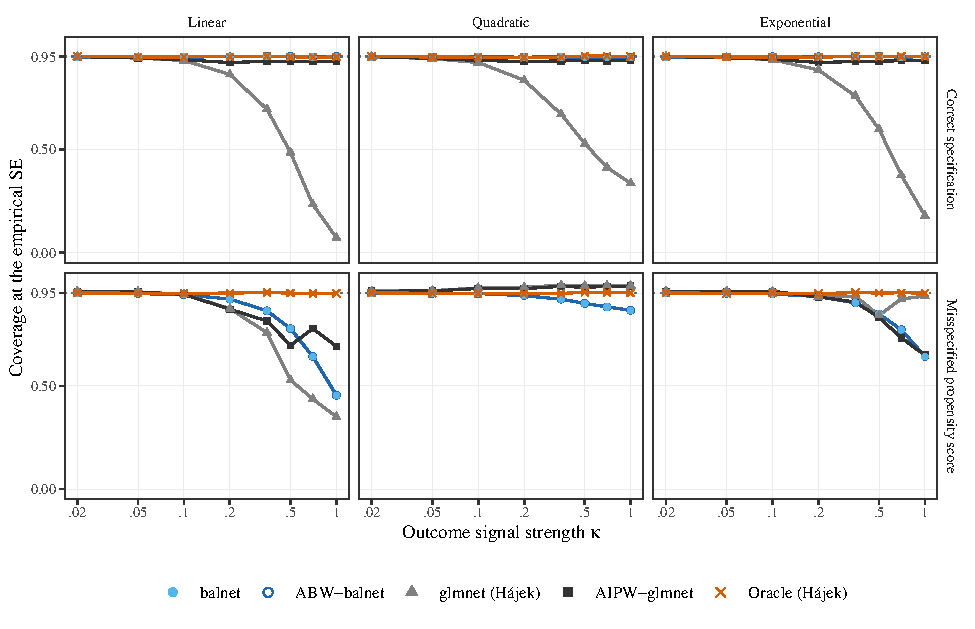
\includegraphics[keepaspectratio]{AAAAA-Working-Thesis_files/figure-pdf/unnamed-chunk-28-1.pdf}}

}

\caption{\label{afig-sig-coverage}Coverage at the empirical SE by
outcome signal strength \(\kappa\) at \(n\) = 1000, both specifications.
The dotted line is the nominal 95\%.}

\end{afig}%

\subsection*{Appendix H: Wong--Chan design}\label{sec-app-wc}
\addcontentsline{toc}{subsection}{Appendix H: Wong--Chan design}

The design of Wong and Chan (2018) as run by Wang and Zubizarreta (2020)
has ten standard normal covariates, a logistic treatment on two, outcome
model A linear in four and model B nonlinear in them, and an analyst who
sees Kang--Schafer transforms of the four. We use \(n\) = 5000, the ATT
and 1000 replications, \texttt{balnet} balancing the covariates and
their squares on a 100-point \(\lambda\) grid, the logit scaled by 1, 2
or 4 and the noise SD \(\sigma\) at 1, 10, 30 and 100. Cells match DGP
2's misspecified grid on the SD of the true logit (\(c\) = 1, 0.5, 0.25)
and on \(R^2_e\), the share of the control outcome's variance the true
score explains, which neither overlap knob changes. The endpoint is the
last \(\lambda\) reached by 95\% of replications for Wong--Chan and each
replication's own last \(\lambda\) for DGP 2.

\begin{afig}

\centering{

\pandocbounded{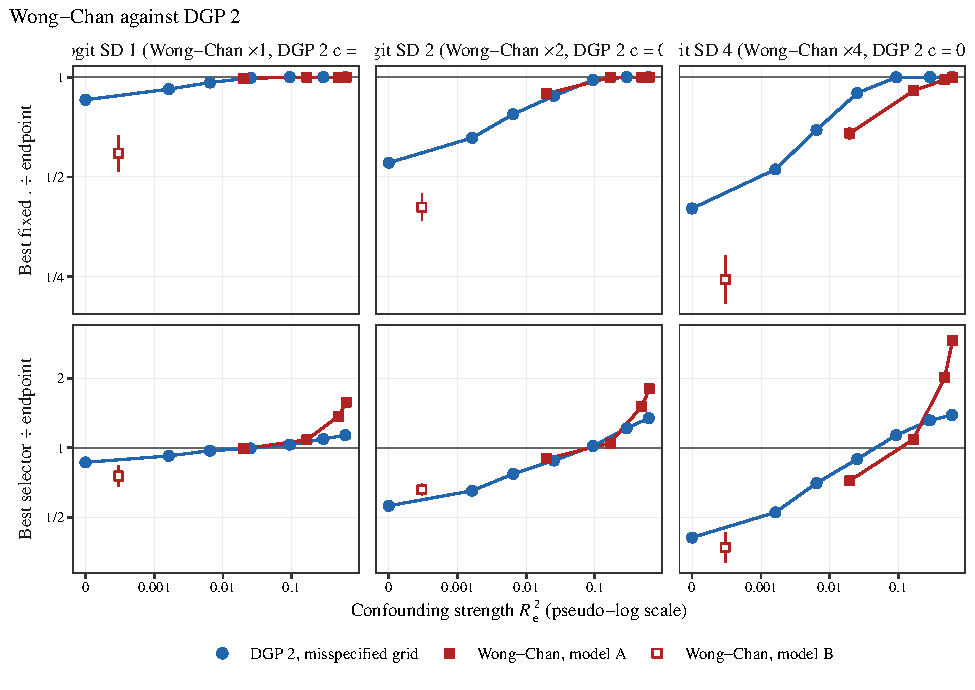
\includegraphics[keepaspectratio]{AAAAA-Working-Thesis_files/figure-pdf/unnamed-chunk-29-1.pdf}}

}

\caption{\label{afig-app-wc}RMSE at the best fixed \(\lambda\) (top) and
of the best selector (bottom), relative to the endpoint's, against
\(R^2_e\) by logit SD. Wong--Chan points are model A at \(\sigma\) =
100, 30, 10 and 1 (left to right) and model B at \(\sigma\) = 1 (open),
DGP 2 points \(\kappa\) = 0 to 1 under the linear outcome.}

\end{afig}%

\begin{atbl}

\caption{\label{atbl-app-wc}Interior optima and selector wins, each
Wong--Chan cell against the DGP 2 cells bracketing its \(R^2_e\) at the
same logit SD.}

\centering{

\begingroup
\fontsize{8.0pt}{10.0pt}\selectfont
\setlength{\LTpost}{0mm}
\begin{longtable*}{llrrrrcccc}
\toprule
\multicolumn{2}{c}{{Matched cells (\(R^2_e\))}} & \multicolumn{2}{c}{{Best fixed \(\lambda\)}} & \multicolumn{2}{c}{{Best selector}} & \multicolumn{2}{c}{{Interior optimum}} & \multicolumn{2}{c}{{Selector win}} \\ 
\cmidrule(lr){1-2} \cmidrule(lr){3-4} \cmidrule(lr){5-6} \cmidrule(lr){7-8} \cmidrule(lr){9-10}
Wong–Chan & DGP 2 & W–C & DGP 2 & W–C & DGP 2 & W–C & DGP 2 & W–C & DGP 2 \\ 
\midrule\endhead\addlinespace[2.5pt]
\multicolumn{10}{l}{{\bfseries Propensity logit SD 1 (Wong–Chan ×1, DGP 2 c = 1)}} \\[2.5pt] 
\midrule\addlinespace[2.5pt]
B, \(\sigma\) = 1 (0.0003) & \(\kappa\) = 0 (0) & 0.59 & 0.85 & 0.75 & 0.86 & yes & yes & yes & yes \\ 
A, \(\sigma\) = 100 (0.020) & \(\kappa\) = 1/16--1/8 (0.0065--0.025) & 0.99 & 0.96–0.99 & 0.99 & 0.97–0.99 & no & no & no & no \\ 
A, \(\sigma\) = 30 (0.17) & \(\kappa\) = 1/4--1/2 (0.094--0.29) & 1.00 & 1.00 & 1.08 & 1.03–1.09 & no & no & no & no \\ 
A, \(\sigma\) = 10 (0.48) & \(\kappa\) = 1/2--1 (0.29--0.61) & 1.00 & 1.00 & 1.37 & 1.09–1.13 & no & no & no & no \\ 
A, \(\sigma\) = 1 (0.62) & \(\kappa\) = 1 (0.61) & 1.00 & 1.00 & 1.57 & 1.13 & no & no & no & no \\ 
\midrule\addlinespace[2.5pt]
\multicolumn{10}{l}{{\bfseries Propensity logit SD 2 (Wong–Chan ×2, DGP 2 c = 0.5)}} \\[2.5pt] 
\midrule\addlinespace[2.5pt]
B, \(\sigma\) = 1 (0.0003) & \(\kappa\) = 0 (0) & 0.41 & 0.55 & 0.66 & 0.56 & yes & yes & yes & yes \\ 
A, \(\sigma\) = 100 (0.020) & \(\kappa\) = 1/16--1/8 (0.0065--0.025) & 0.89 & 0.77–0.88 & 0.90 & 0.77–0.88 & yes & yes & yes & yes \\ 
A, \(\sigma\) = 30 (0.17) & \(\kappa\) = 1/4--1/2 (0.094--0.29) & 1.00 & 0.98–1.00 & 1.05 & 1.02–1.21 & no & no & no & no \\ 
A, \(\sigma\) = 10 (0.48) & \(\kappa\) = 1/2--1 (0.29--0.61) & 1.00 & 1.00 & 1.51 & 1.21–1.34 & no & no & no & no \\ 
A, \(\sigma\) = 1 (0.62) & \(\kappa\) = 1 (0.61) & 1.00 & 1.00 & 1.80 & 1.34 & no & no & no & no \\ 
\midrule\addlinespace[2.5pt]
\multicolumn{10}{l}{{\bfseries Propensity logit SD 4 (Wong–Chan ×4, DGP 2 c = 0.25)}} \\[2.5pt] 
\midrule\addlinespace[2.5pt]
B, \(\sigma\) = 1 (0.0003) & \(\kappa\) = 0 (0) & 0.25 & 0.40 & 0.37 & 0.41 & yes & yes & yes & yes \\ 
A, \(\sigma\) = 100 (0.020) & \(\kappa\) = 1/16--1/8 (0.0065--0.025) & 0.68 & 0.69–0.90 & 0.72 & 0.70–0.89 & yes & yes & yes & yes \\ 
A, \(\sigma\) = 30 (0.17) & \(\kappa\) = 1/4--1/2 (0.094--0.29) & 0.91 & 1.00 & 1.09 & 1.13–1.31 & yes & no & no & no \\ 
A, \(\sigma\) = 10 (0.48) & \(\kappa\) = 1/2--1 (0.29--0.61) & 0.98 & 1.00 & 2.02 & 1.31–1.39 & no & no & no & no \\ 
A, \(\sigma\) = 1 (0.62) & \(\kappa\) = 1 (0.61) & 1.00 & 1.00 & 2.92 & 1.39 & no & no & no & no \\ 
\bottomrule
\end{longtable*}
\begin{minipage}{\linewidth}
\vspace{.05em}
Ratios: RMSE at the best fixed \(\lambda\) on the path, and of the best of the five shared selectors, over RMSE at the path endpoint; below 1 the endpoint is beaten. Each Wong--Chan cell is set against the cells of DGP 2's misspecified grid at the same logit SD whose \(R^2_e\) (in brackets) bracket its own, model B against \(\kappa\) = 0; a DGP 2 entry spans its two cells. Interior optimum and selector win as defined in Performance measures, applied to both designs. The designs agree on the interior optimum in 14 of 15 matched cells and on the selector win in 15 of 15; the exception: logit SD 4, \(\sigma\) = 30 (interior optimum yes against no). Largest MCSE of a log ratio 0.085 (Wong--Chan), 0.019 (DGP 2).\\
\end{minipage}
\endgroup

}

\end{atbl}%

\subsection*{Appendix I: Study 2}\label{sec-app-s2}
\addcontentsline{toc}{subsection}{Appendix I: Study 2}

\begin{atbl}

\caption{\label{atbl-s2-selectors}Selector wins, lowest RMSE and mean
RMSE change by selector, all Study 2 grids.}

\centering{

\begingroup
\fontsize{8.0pt}{10.0pt}\selectfont
\setlength{\LTpost}{0mm}
\begin{longtable*}{lllrrrrrrrr}
\toprule
 &  &  & \multicolumn{2}{c}{{Selector win (\%)}} & \multicolumn{2}{c}{{Win given an interior optimum (\%)}} & \multicolumn{2}{c}{{Lowest RMSE (\%)}} & \multicolumn{2}{c}{{Mean RMSE change (\%)}} \\ 
\cmidrule(lr){4-5} \cmidrule(lr){6-7} \cmidrule(lr){8-9} \cmidrule(lr){10-11}
Selector & Criterion & Scoring & balnet & ABW & balnet & ABW & balnet & ABW & balnet & ABW \\ 
\midrule\endhead\addlinespace[2.5pt]
\texttt{cv.bloss} & \texttt{bloss} & Cross-validation & 54 & 74 & 89 & 93 & 26 & 25 & -1 & -16 \\ 
\texttt{cv.smd} & \texttt{smd} & Cross-validation & 40 & 50 & 65 & 63 & 15 & 19 & 30 & -7 \\ 
\texttt{cv.inf} & \texttt{inf} & Cross-validation & 43 & 55 & 70 & 70 & 16 & 20 & 16 & -13 \\ 
\texttt{boot.smd} & \texttt{smd} & Bootstrap & 38 & 51 & 63 & 64 & 13 & 11 & 11 & -11 \\ 
\texttt{boot.inf} & \texttt{inf} & Bootstrap & 52 & 70 & 85 & 89 & 30 & 25 & -5 & -15 \\ 
\bottomrule
\end{longtable*}
\begin{minipage}{\linewidth}
\vspace{.05em}
Shares of the 1803 cells per estimator over the ten Study 2 grids. Selector win: RMSE below the endpoint's by more than three times their combined MCSE. Lowest RMSE: lowest of the five in the cell, whether or not it wins. Mean RMSE change: geometric mean of the selector's RMSE over the endpoint's, all cells.\\
\end{minipage}
\endgroup

}

\end{atbl}%

\subsubsection*{Penalty form}\label{penalty-form}
\addcontentsline{toc}{subsubsection}{Penalty form}

\begin{atbl}

\caption{\label{atbl-s2-alpha}Interior optima, selector wins and RMSE
relative to the lasso by penalty form \(\alpha\).}

\centering{

\begingroup
\fontsize{8.0pt}{10.0pt}\selectfont
\setlength{\LTpost}{0mm}
\begin{longtable*}{lrrrrrrrr}
\toprule
 & \multicolumn{2}{c}{{Interior optimum (\%)}} & \multicolumn{2}{c}{{Selector win (\%)}} & \multicolumn{2}{c}{{RMSE / lasso, endpoint}} & \multicolumn{2}{c}{{RMSE / lasso, optimum}} \\ 
\cmidrule(lr){2-3} \cmidrule(lr){4-5} \cmidrule(lr){6-7} \cmidrule(lr){8-9}
\(\alpha\) & balnet & ABW & balnet & ABW & balnet & ABW & balnet & ABW \\ 
\midrule\endhead\addlinespace[2.5pt]
1 (lasso) & 60 & 85 & 56 & 82 & 1.00 & 1.00 & 1.00 & 1.00 \\ 
0.75 & 63 & 86 & 55 & 83 & 1.05 & 0.91 & 1.02 & 0.94 \\ 
0.5 & 55 & 85 & 51 & 85 & 1.07 & 0.89 & 1.06 & 0.92 \\ 
0.25 & 51 & 69 & 49 & 64 & 1.08 & 0.83 & 1.08 & 0.89 \\ 
0 (ridge) & 61 & 86 & 55 & 83 & 1.08 & 0.91 & 1.08 & 0.89 \\ 
\bottomrule
\end{longtable*}
\begin{minipage}{\linewidth}
\vspace{.05em}
Shares over the 84 cells per \(\alpha\) and estimator (four overlaps, seven \(\kappa\), three outcomes). Ratios: geometric mean over the 18 cells at \(c \le 0.25\) and \(\kappa\) = 1 of the RMSE at the endpoint, or at the path minimum, to the lasso's in the same cell. The endpoints differ by construction and the forms do not share draws. With no signal every \(\alpha < 1\) lowers the endpoint RMSE of both estimators by 13\% to 24\%, and at \(c\) = 1 every form stays within 3\% of the lasso at both points.\\
\end{minipage}
\endgroup

}

\end{atbl}%

\subsubsection*{Sample size and
dimension}\label{sample-size-and-dimension}
\addcontentsline{toc}{subsubsection}{Sample size and dimension}

\begin{afig}

\centering{

\pandocbounded{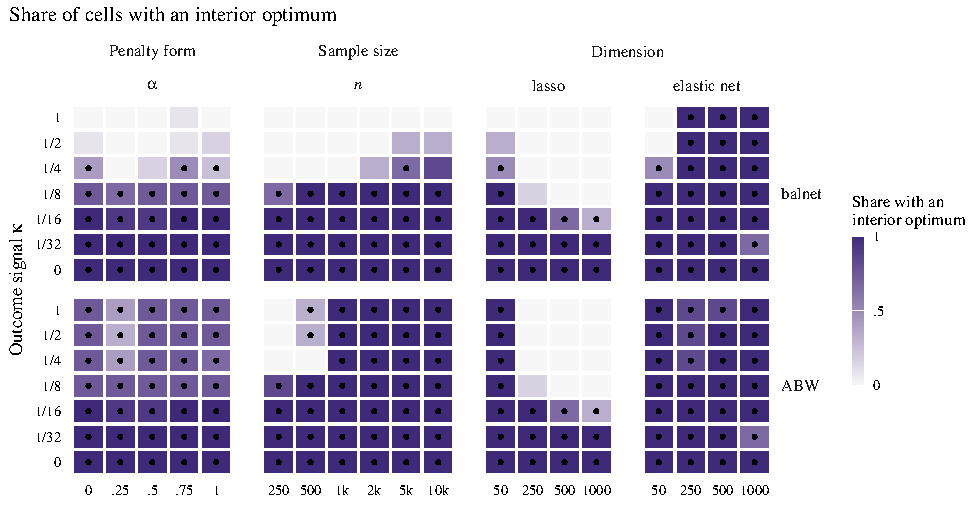
\includegraphics[keepaspectratio]{AAAAA-Working-Thesis_files/figure-pdf/unnamed-chunk-33-1.pdf}}

}

\caption{\label{afig-s2-design}Share of cells with an interior optimum
by \(\kappa\) and \(\alpha\), \(n\) or \(p\), pooled over each grid's
outcomes and overlap levels (Table~\ref{tbl-grids-s2}). A dot marks a
selector win in any pooled cell.}

\end{afig}%

\subsubsection*{Misspecification and denser
confounders}\label{misspecification-and-denser-confounders}
\addcontentsline{toc}{subsubsection}{Misspecification and denser
confounders}

\begin{afig}

\centering{

\pandocbounded{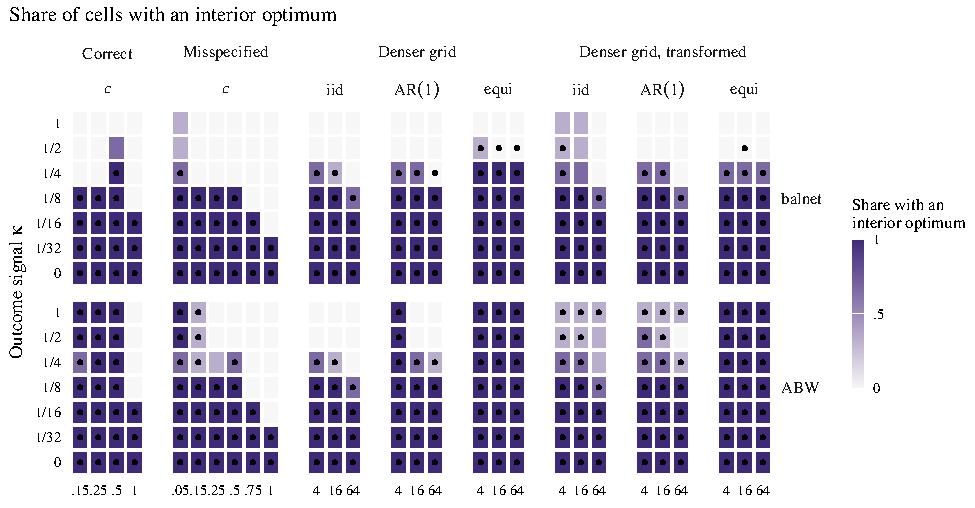
\includegraphics[keepaspectratio]{AAAAA-Working-Thesis_files/figure-pdf/unnamed-chunk-34-1.pdf}}

}

\caption{\label{afig-s2-spec}As Appendix Figure~\ref{afig-s2-design}, by
\(c\) under each specification and by \(s\) and covariance structure in
the denser grid, with and without Tan's transformation.}

\end{afig}%




\end{document}
